\section{Continuous Integration/Delivery}
\subsection{GitHub Actions}

allg. actions warum kosten
\subsubsection{iOS Build} \setauthor{Martin Hausleitner} Das
Ziel des Projekts war es, eine \cite{ios_app_store} iOS-App
im App Store zu veröffentlichen und eine

% \cite{android_play_store} 

Android-App im Play Store anzubieten. Da Martin Hausleitner der einzige im Team war, der ein iPhone besaß und Erfahrungen mit Apple hatte, übernahm er die Verantwortung für den Build-Prozess der iOS-App.
Zur Erstellung einer \cite{flutter} Flutter iOS-App ein Mac mit \cite{xcode} Xcode sowie ein \cite{apple_developer_program} Apple-Entwicklerkonto erforderlich. Da jedoch niemand im Team über ein solches Konto verfügte, gestaltete sich der Build-Prozess äußerst schwierig. Glücklicherweise konnte Martin Hausleitner einen alten iMac von seiner Familie ausleihen, auf dem er arbeiten konnte. Obwohl das Erstellen einer iOS-App auf den ersten Blick einfach erscheint, stellte es sich als eine der größten Herausforderungen in diesem Projekt heraus.
Da MacOS und Xcode dem Entwickler nicht vertraut waren, musste er sich zunächst mühsam einarbeiten. Es bedurfte zahlreicher Anläufe, um die App zum ersten Mal zu erstellen, da zum damaligen Zeitpunkt von Flutter noch keine vorgefertigten Build-Abläufe zur Verfügung standen.


\paragraph{Github Action}\mbox{} \\
Es war eine mühsame Aufgabe, Xcode zu konfigurieren, und
nach mehreren Versuchen wurde schließlich die erste
.ipa-Datei erstellt. Allerdings war der schwierigste Teil
noch nicht überwunden, da das Ziel darin bestand, bei jedem
GitHub-Push automatisch eine iOS-App zu erstellen.

Um über GitHub Actions eine iOS-App zu erstellen, sind
mehrere Actions-Secrets erforderlich, die aus Xcode bezogen
werden müssen. Folgende Secrets waren notwendig:

\begin{itemize}
  \item \verb|BUILD_CERTIFICATE_BASE64:| Dieses Secret enthält das Zertifikat, das zur Signierung der iOS-App verwendet wird. Es muss von einer vertrauenswürdigen Zertifizierungsstelle ausgestellt worden sein und wird normalerweise als Base64-codierte Zeichenfolge bereitgestellt.
  \item \verb|BUILD_PROVISION_PROFILE_BASE64:| Dieses Secret enthält das Provisioning-Profil, das zur Installation der iOS-App auf einem Gerät oder für die Verwendung von Testflight verwendet wird. Das Provisioning-Profil enthält Informationen über die Geräte, auf denen die App installiert werden kann, sowie das verwendete Zertifikat. Auch dieses Secret wird normalerweise als Base64-codierte Zeichenfolge bereitgestellt.
  \item \verb|KEYCHAIN_PASSWORD:| Dieses Secret ist das Passwort für den Zugriff auf den Schlüsselbund, in dem das Signaturzertifikat und der dazugehörige private Schlüssel gespeichert sind. Der private Schlüssel wird benötigt, um die App zu signieren, und das Passwort schützt den Zugriff auf den Schlüsselbund vor unbefugtem Zugriff.
  \item \verb|P12_PASSWORD:| Dieses Secret ist das Passwort für das PKCS\#12-Dateiformat, das das Signaturzertifikat und den privaten Schlüssel enthält. Diese Datei wird normalerweise für die Signierung von iOS-Apps verwendet. Das Passwort schützt die Datei vor unbefugtem Zugriff und stellt sicher, dass nur autorisierte Personen Zugriff auf den privaten Schlüssel haben.
\end{itemize}

Nach mehreren Versuchen, die Actions funktionsfähig zu
machen, gelang es schließlich, eine .ipa-Datei zu erstellen.

\paragraph{Firebase App Distribution}\mbox{} \\
Für die Testphase und die Beta-Version der iOS-App nutzten
wir, wie auch bei der Android-App, Firebase App
Distribution. Beim Hochladen der .ipa-Dateien gab es
allerdings Probleme mit den Zertifikaten.

\paragraph{Apple Developer Lizenz}\mbox{} \\
Um eine .ipa-Datei auf einem iOS-Gerät auszuführen, ist eine verifizierte .ipa-Datei erforderlich. Die aktuelle Action konnte die App jedoch nur mit der lokalen Entwicklerlizenz verifizieren, um sie im Emulator auf MacOS auszuführen. Wenn die App also auf einem anderen Gerät installiert werden sollte, war dies nicht möglich. Dies war auch der Grund, warum der Upload auf Firebase App Distribution nicht funktionierte.

Es gibt verschiedene Möglichkeiten, um eine .ipa-Datei zur
Verfügung zu stellen, darunter:

\begin{itemize}
  \item \textbf{App Store-Verteilung}: Die offizielle Methode zur Verteilung von iOS-Apps an eine globale Benutzerbasis. Apple prüft jede App, bevor sie im App Store veröffentlicht wird.
  \item \textbf{Ad-Hoc-Verteilung}: Die Ad-Hoc-Verteilung ermöglicht es Entwicklern, ihre Apps an eine begrenzte Anzahl von Personen außerhalb des App Stores zu verteilen. Entwickler müssen die UDIDs der Testgeräte manuell registrieren und eine Ad-Hoc-Provisioning-Datei erstellen, die zusammen mit der App an die Tester gesendet wird.
  \item \textbf{TestFlight-Verteilung}: TestFlight ist eine kostenlose Plattform von Apple, die es Entwicklern ermöglicht, ihre Apps an ausgewählte Tester zu verteilen. Jeder Tester lädt einfach TestFlight herunter, meldet sich mit seiner Apple-ID an und erhält Zugriff auf die App.
  \item \textbf{Enterprise-Verteilung}: Die Enterprise-Verteilung ermöglicht es Unternehmen, ihre Apps intern an Mitarbeiter oder Kunden zu verteilen, ohne den App Store zu nutzen. Sie benötigen jedoch eine spezielle Enterprise-Entwicklerlizenz von Apple und müssen die Apps auf einem eigenen Unternehmens-Server hosten.
  \item \textbf{B2B-Verteilung}: Die B2B-Verteilung ermöglicht es Entwicklern, ihre Apps speziell für Unternehmen und Organisationen zu entwickeln und diese direkt an diese Kunden zu verkaufen. Die Apps können dann über den App Store oder über ein spezielles B2B-Programm verkauft werden.
  \item \textbf{TestFlight für interne Tests}: TestFlight für interne Tests ist ähnlich wie die öffentliche TestFlight-Verteilung, jedoch speziell für interne Tests in Unternehmen. Diese Methode erfordert jedoch ein Apple Developer Enterprise-Programm.
  \item \textbf{Sideloading}: Sideloading ist eine Methode, bei der eine App von einem Drittanbieter auf einem iOS-Gerät installiert werden kann. Diese Methode erfordert jedoch, dass die Sicherheitseinstellungen des Geräts geändert werden und die App möglicherweise nicht von Apple genehmigt wurde.
\end{itemize}

Zunächst wurde die Methode des Sideloading mittels des
Tools \cite{signulous} Signulous ausprobiert,
da sie als kostenfreie Option bekannt war. Dabei konnte
die iOS-Anwendung erfolgreich installiert werden und
manuelle Uploads auf Firebase App Distribution waren
ebenfalls möglich. Um jedoch eine Automatisierung zu
ermöglichen, musste eine andere Lösung gefunden werden.

Da die HTL Leonding ihren Schülerinnen und Schülern Entwickler-Accounts zur Verfügung stellt, hat das Team um Zugriff auf einen solchen Account. Allerdings wurde dieser Account so eingeschränkt, dass es nicht möglich war, die Anwendung zu verifizieren. Nach weiteren Anfragen bezüglich einer Erweiterung der Berechtigungen für die Verifizierung wurde klar, dass dies nicht möglich war.

Somit blieb nur noch die Möglichkeit, einen kostenpflichtigen Entwickler-Account für \$99 pro Jahr zu erwerben. Das Team entschied sich jedoch dagegen, da der Aufwand bereits zu hoch war und weitere Zeit verschwendet würde.

Dennoch wurde versucht, auf TestFlight umzusteigen, was jedoch ebenfalls den Kauf eines Entwickler-Accounts erforderte. Sobald die Android-Version mit ihren Funktionen weiterentwickelt ist, plant das Team, die Arbeit an der iOS-Version wieder aufzunehmen, um die Anwendung im App Store zu veröffentlichen.


% \textbf{BUILD_PROVISION_PROFILE_BASE64}: Dieses Secret enthält das Provisioning-Profil, das zur Installation der iOS-App auf einem Gerät oder für die Verwendung von Testflight verwendet wird. Das Provisioning-Profil enthält Informationen über die Geräte, auf denen die App installiert werden kann, sowie das verwendete Zertifikat. Auch dieses Secret wird normalerweise als Base64-codierte Zeichenfolge bereitgestellt.

% \textbf{KEYCHAIN_PASSWORD}: Dieses Secret ist das Passwort für den Zugriff auf den Schlüsselbund, in dem das Signaturzertifikat und der dazugehörige private Schlüssel gespeichert sind. Der private Schlüssel wird benötigt, um die App zu signieren, und das Passwort schützt den Zugriff auf den Schlüsselbund vor unbefugtem Zugriff.

% \textbf{P12_PASSWORD}: Dieses Secret ist das Passwort für das PKCS#12-Dateiformat, das das Signaturzertifikat und den privaten Schlüssel enthält. Diese Datei wird normalerweise für die Signierung von iOS-Apps verwendet. Das Passwort schützt die Datei vor unbefugtem Zugriff und stellt sicher, dass nur autorisierte Personen Zugriff auf den privaten Schlüssel haben.


% \begin{itemize}
%   \begin{description}[style=nextline,format=--- \textbf]
%     \item[The first] \textbf{BUILD_CERTIFICATE_BASE64}: Dieses Secret enthält das Zertifikat, das zur Signierung der iOS-App verwendet wird. Es muss von einer vertrauenswürdigen Zertifizierungsstelle ausgestellt worden sein und wird normalerweise als Base64-codierte Zeichenfolge bereitgestellt.
%     \item \textbf{pages} - Hier werden Widgets entworfen, die jeweils eine Seite der App darstellen.
%     \item \textbf{routes} - Hier werden die Routen definiert, die tiefere Links ermöglichen.
%     \item \textbf{shared} - Hier werden UI-Widgets wie Buttons oder andere Widgets gespeichert, die oft wiederverwendet werden.
%     \item \textbf{views} - Hier befinden sich Ansichten, die von mehreren Seiten der App verwendet werden können.
%   \end{description}
% \end{itemize}





\subsubsection{Build Android}

\subsection{Fastline}
\subsubsection{Build Number increment}
\subsection{Firebase App Distribution}

\section{Mobile Anwendung}
\subsection{Dateistruktur}
\setauthor{Martin Hausleitner}
Bei der Entwicklung einer Flutter-App gibt es keine vorgegebene Dateistruktur. Stattdessen können Entwickler ihre eigene Struktur entwerfen und gestalten. Im Folgenden wird beschrieben, wie die Dateistruktur für das betreffende Flutter-Projekt aufgebaut wurde.

Da es keine festen Vorgaben gibt, kann man sich bei der
Strukturierung an bewährten Praktiken orientieren. In diesem
Fall wurde die Dateistruktur so gewählt, dass sie effizient,
übersichtlich und gut organisiert ist, um eine reibungslose
Entwicklung und Wartung der App zu ermöglichen.


Die Dateistruktur sieht wie folgt aus:

\begin{itemize}
  \item \textbf{logic} - Hier befindet sich die Geschäftslogik der App, einschließlich der Firestore-Cloud-Funktionen und Repositories, die API-Aufrufe ausführen.
  \item \textbf{pages} - Hier werden Widgets entworfen, die jeweils eine Seite der App darstellen.
  \item \textbf{routes} - Hier werden die Routen definiert, die tiefere Links ermöglichen.
  \item \textbf{shared} - Hier werden UI-Widgets wie Buttons oder andere Widgets gespeichert, die oft wiederverwendet werden.
  \item \textbf{views} - Hier befinden sich Ansichten, die von mehreren Seiten der App verwendet werden können.
\end{itemize}

Rückblickend wäre es möglich, die Dateistruktur anders zu gestalten, beispielsweise durch die Definition des UI als eigenes Package und eine bessere Unterteilung der Pages und Views. Diese Anpassungen könnten zu einer noch übersichtlicheren und besser organisierten Struktur beitragen.

\subsection{State Management}
In Flutter gibt es verschiedene Möglichkeiten\cite{flutter-docs-interactive}\cite{flutter-state-management-blog}, um mit dem State Management umzugehen. State Management bezieht sich auf die Art und Weise, wie Daten innerhalb einer App verwaltet werden. In jeder App gibt es bestimmte Daten, die von verschiedenen Komponenten und Widgets verwendet werden und sich im Laufe der Zeit ändern können. State Management bezieht sich auf die Methoden, die verwendet werden, um diese Daten innerhalb der App zu verwalten und zu aktualisieren.
\setauthor{Martin Hausleitner}

\subsubsection{GetX}
\setauthor{Martin Hausleitner}

GetX verwendet ein reaktives Ansatz zur Verwaltung des Zustands, was bedeutet, dass Änderungen im Zustand automatisch die UI aktualisieren, ohne dass der Entwickler manuell Code schreiben muss, um diese Aktualisierungen durchzuführen. Dies spart viel Entwicklungszeit und macht es einfach, auf Benutzerinteraktionen zu reagieren.

Mit GetX lässt sich eine einheitliche Datenquelle erstellen, auf die alle Komponenten zugreifen können. Dies erleichtert die Wartung und Erweiterung der Anwendung. Zudem bietet GetX eine einfache Möglichkeit, Abhängigkeiten zu verwalten und Zustandsinformationen zwischen verschiedenen Bildschirmen zu teilen. Diese Funktionen tragen zu einer effizienteren und besser strukturierten App-Entwicklung bei.

Insgesamt hat die Verwendung von GetX im Flutter-Framework wesentlich dazu beigetragen, eine effektive und skalierbare Anwendung zu entwickeln, die auf die Bedürfnisse der Benutzer zugeschnitten ist.


\setauthor{Sandin Habibovic}

GetX verfügt über zwei wichtige Konzepte: GetxController und GetxService

\subsubsection{GetxController}
\setauthor{Sandin Habibovic}
GetxController ist eine Klasse, die verwendet wird, um den Zustand eines Widgets oder einer Gruppe von Widgets zu verwalten. Ein GetxController ähnelt dem StatefulWidget von Flutter, bietet jedoch zusätzliche Funktionen wie reaktive Programmierung und Dependency Injection. GetxController werden verwendet, um die Logik eines Widgets von seiner Präsentation zu trennen, was das Warten und Testen vereinfachen soll.
\\
GetxController bieten einige Vorteile. Dazu gehören:
\\
\textbf{Einfachheit:}
GetxController sind einfach zu verstehen und zu implementieren und erfordern keine zusätzlichen Boilerplate-Code oder das Erlernen von komplexen Konzepten, um es in einer Anwendung zu verwenden.
\\
\textbf{Flexibilität:}
GetxController können in jeder Flutter-Anwendung verwendet werden, unabhängig von ihrer Größe oder Komplexität. Es kann leicht in bestehende Projekte integriert oder für neue Anwendungen verwendet werden.
\\
\textbf{Kapselung:}
GetxController kapseln den Zustand und die Logik der Anwendung und ermöglichen eine saubere Trennung von Zuständigkeiten. Dadurch wird der Code besser organisiert und wartbarer.
\\
\begin{lstlisting}[caption=Beispiel zum Einsatz von einem GetxController in Kombination mit GetView,label=lst:GetxControllerExample]
  import 'package:get/get.dart';

  class HomeController extends GetxController {
    var counter = 0;

    void incrementCounter() {
      counter++;
      update();
    }
  }

  class HomePage extends GetView<HomeController> {
    const HomePage({Key? key}) : super(key: key);

    @override
    Widget build(BuildContext context) {
      return Scaffold(
        appBar: AppBar(
          title: const Text('Home Page'),
        ),
        body: Center(
          child: Column(
            mainAxisAlignment: MainAxisAlignment.center,
            children: [
              GetBuilder<HomeController>(
                builder: (_) {
                  return Text(
                    'Counter: ${controller.counter}',
                    style: TextStyle(fontSize: 24),
                  );
                },
              ),
              SizedBox(height: 16),
              ElevatedButton(
                onPressed: controller.incrementCounter,
                child: Text('Increment'),
              ),
            ],
          ),
        ),
      );
    }
  }
\end{lstlisting}
Der vorliegende Code \ref{lst:GetxControllerExample} ist ein beispielhafter Code, der demonstrieren soll wie ein GetxController in Kombination mit einem GetView verwendet werden kann, um reaktive Funktionalität in einer Flutter-App zu implementieren.
\\
Der HomeController ist eine Klasse, die von GetxController erbt. Die Klasse definiert eine Eigenschaft \textit{counter} und eine Methode \textit{incrementCounter()}, die den Wert der Eigenschaft um 1 erhöht und \textit{update()} aufruft. \textit{update()} ist eine Methode von GetxController, die dem jeweiligen Widget mitteilt, dass das UI aktualisiert werden soll.
\\
Die HomePage-Klasse erbt von einem GetView-Widget, welches den HomeController implementiert hat. Die GetView-Klasse hat eine eingebaute Variable namens \textit{controller}, die den Zugriff auf den HomeController ermöglicht.


\subsubsection{GetxService}
\setauthor{Sandin Habibovic}
GetxService ist eine Klasse, die eine globale Instanz eines Dienstes bereitstellt, die in der gesamten Anwendung verwendet werden kann. GetxService werden in der Regel für Operationen verwendet, die einmal ausgeführt werden müssen, wie zum Beispiel das Erstellen, Updaten oder Löschen von Daten in der Datenbanken, API-Aufrufen und anderen Backend-Services. Im Gegensatz zum GetxController bietet GetxService keine automatische Aktualisierung der UI.
\\
Einige Vorteile von GetxServices sind:
\\
\textbf{Langlebigkeit:}
GetxServices bleiben für die gesamte Lebensdauer der App bestehen, was bedeutet, dass sie einmal initialisiert werden und dann für die gesamte Nutzungsdauer der App zur Verfügung stehen. Dies ist besonders nützlich für Dienste, die nicht direkt an das UI gebunden sind und keine ständige Aktualisierung benötigen.
\\
\textbf{Wiederverwendbarkeit:}
GetxServices können in verschiedenen Teilen der Anwendung wiederverwendet werden, ohne dass sie mehrfach initialisiert werden müssen. Dadurch wird der Code effizienter und einfacher zu verwalten.
\\
\textbf{Zentrale Verwaltung:}
GetxServices ermöglichen eine zentrale Verwaltung von Anwendungsdiensten und -ressourcen, wodurch der Code besser organisiert und leichter zu warten ist.
\\
\textbf{Einfache Integration:}
GetxServices können leicht in bestehende Flutter-Projekte integriert werden, ohne dass große Änderungen am Code vorgenommen werden müssen. Dies erleichtert die Migration von bestehenden Projekten zu GetX.

\paragraph{Beispiel}
\begin{lstlisting}[caption=Beispiel zum Einsatz von einem GetxService,label=lst:GetxServiceExample]
  import 'package:get/get.dart';

  class MyService extends GetxService {
    void callService() {
      Get.snackbar('Service', 'The Service was called');
    }
  }

  class HomeController extends GetxController {
    final MyService myService = Get.find<MyService>();
  
    void callService() {
      myService.callService();
    }
  }
  
  class HomePage extends GetView<HomeController> {
    @override
    Widget build(BuildContext context) {
      return Scaffold(
        appBar: AppBar(
          title: const Text('Home Page'),
        ),
        body: Center(
          child: ElevatedButton(
            onPressed: controller.callService,
            child: const Text('Call Service'),
          ),
        ),
      );
    }
  }
  
\end{lstlisting}
Der vorliegende Code \ref{lst:GetxServiceExample} ist ein beispielhafter Code, wie ein GetxService verwendet werden kann, um einen Dienst in einer Flutter-App zu implementieren.
\\
Die MyService-Klasse erbt von GetxService und definiert eine Methode \textit{callService()}. Diese Methode ruft eine Snackbar auf, die dem User eine Meldung anzeigen soll.
\\
Die HomeController-Klasse erbt von GetxController und hat eine Instanz von \textit{MyService} mit Hilfe von \textit{Get.find<MyService>()} initialisiert. Wenn die Methode \textit{callService()} aufgerufen wird, ruft der Controller die Methode \textit{callService()} der MyService-Instanz auf.

\subsubsection{Kriterium zum Einsatz von GetxController und GetxService}
\setauthor{Sandin Habibovic}
Um einen GetxController oder GetxService verwenden zu können, muss der jeweilige GetxController oder der jeweilige GetxService zuerst registriert werden. Dafür stellt GetX sogenannte Bindings zur Verfügung. Diese Bindings erstellen Instanzen von den jeweiligen GetxControllern oder den jeweiligen GetxServices, die dann mit \textit{GetView<Controller>} bzw. \textit{Get.find<Service>()} aufgerufen werden können.

\paragraph{Beispiel}
\begin{lstlisting}[caption=Beispiel von einem Binding,label=lst:GetxBindingExample]
  import 'package:get/get.dart';

  class HomeBinding extends Bindings {
  @override
  void dependencies() {
    Get.put(MyService());
    Get.put(HomeController());
  }
}

\end{lstlisting}

\subsection{Authentifizierung}
\setauthor{Sandin Habibovic}

Bei der Authentifizierung wird zwischen dem Anmelden und dem Registrieren unterschieden.

\subsubsection{Anmeldeprozess}
\setauthor{Sandin Habibovic}

\begin{figure}[h]
  \centering
  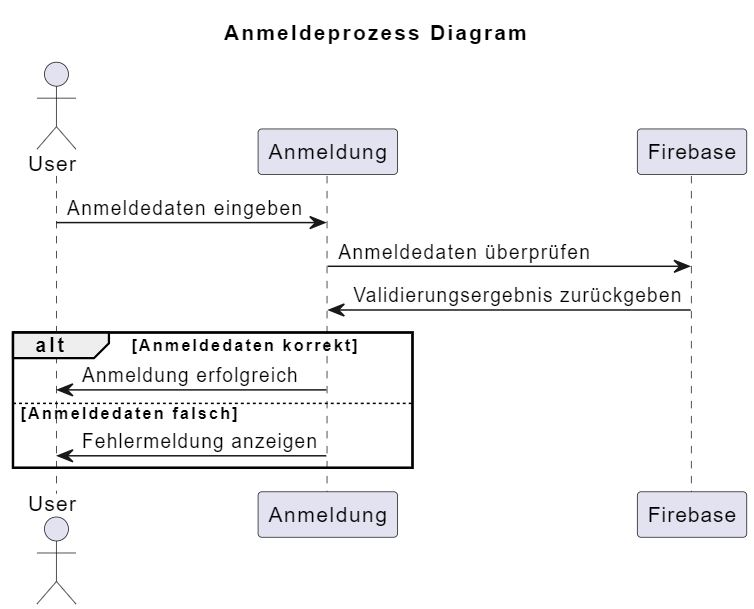
\includegraphics[width=\textwidth]{pics/login-sequence.JPG}
  \caption{Anmeldeprozess}
  \label{fig:login-sequenze}
\end{figure}

Die Abbildung \ref{fig:login-sequenze} repräsentiert ein Sequenzdiagram, welches den Anmeldeprozess für einen User veranschaulichen soll. Der Login-Prozess ist ein wichtiger Schritt in der Benutzerauthentifizierung, bei dem die Identität des Benutzers überprüft wird, um den Zugriff auf die Anwendung zu gewähren oder zu verweigern. Die Anmeldedaten werden an Firebase weitergeleitet, wo diese überprüft werden, um sicherzustellen, dass der User eine gültige E-Mail-Adresse und das korrekte Passwort eingegeben hat.
\\
Falls der User falsche Anmeldedaten eingegeben hat, wird eine Fehlermeldung angezeigt, die den User darauf hinweist, dass die Anmeldedaten falsch sind.
\\
Die Abbildung \ref{fig:login-page} zeigt, wie die Login-Seite in der App dargestellt wird.

\begin{figure}[h]
  \centering
  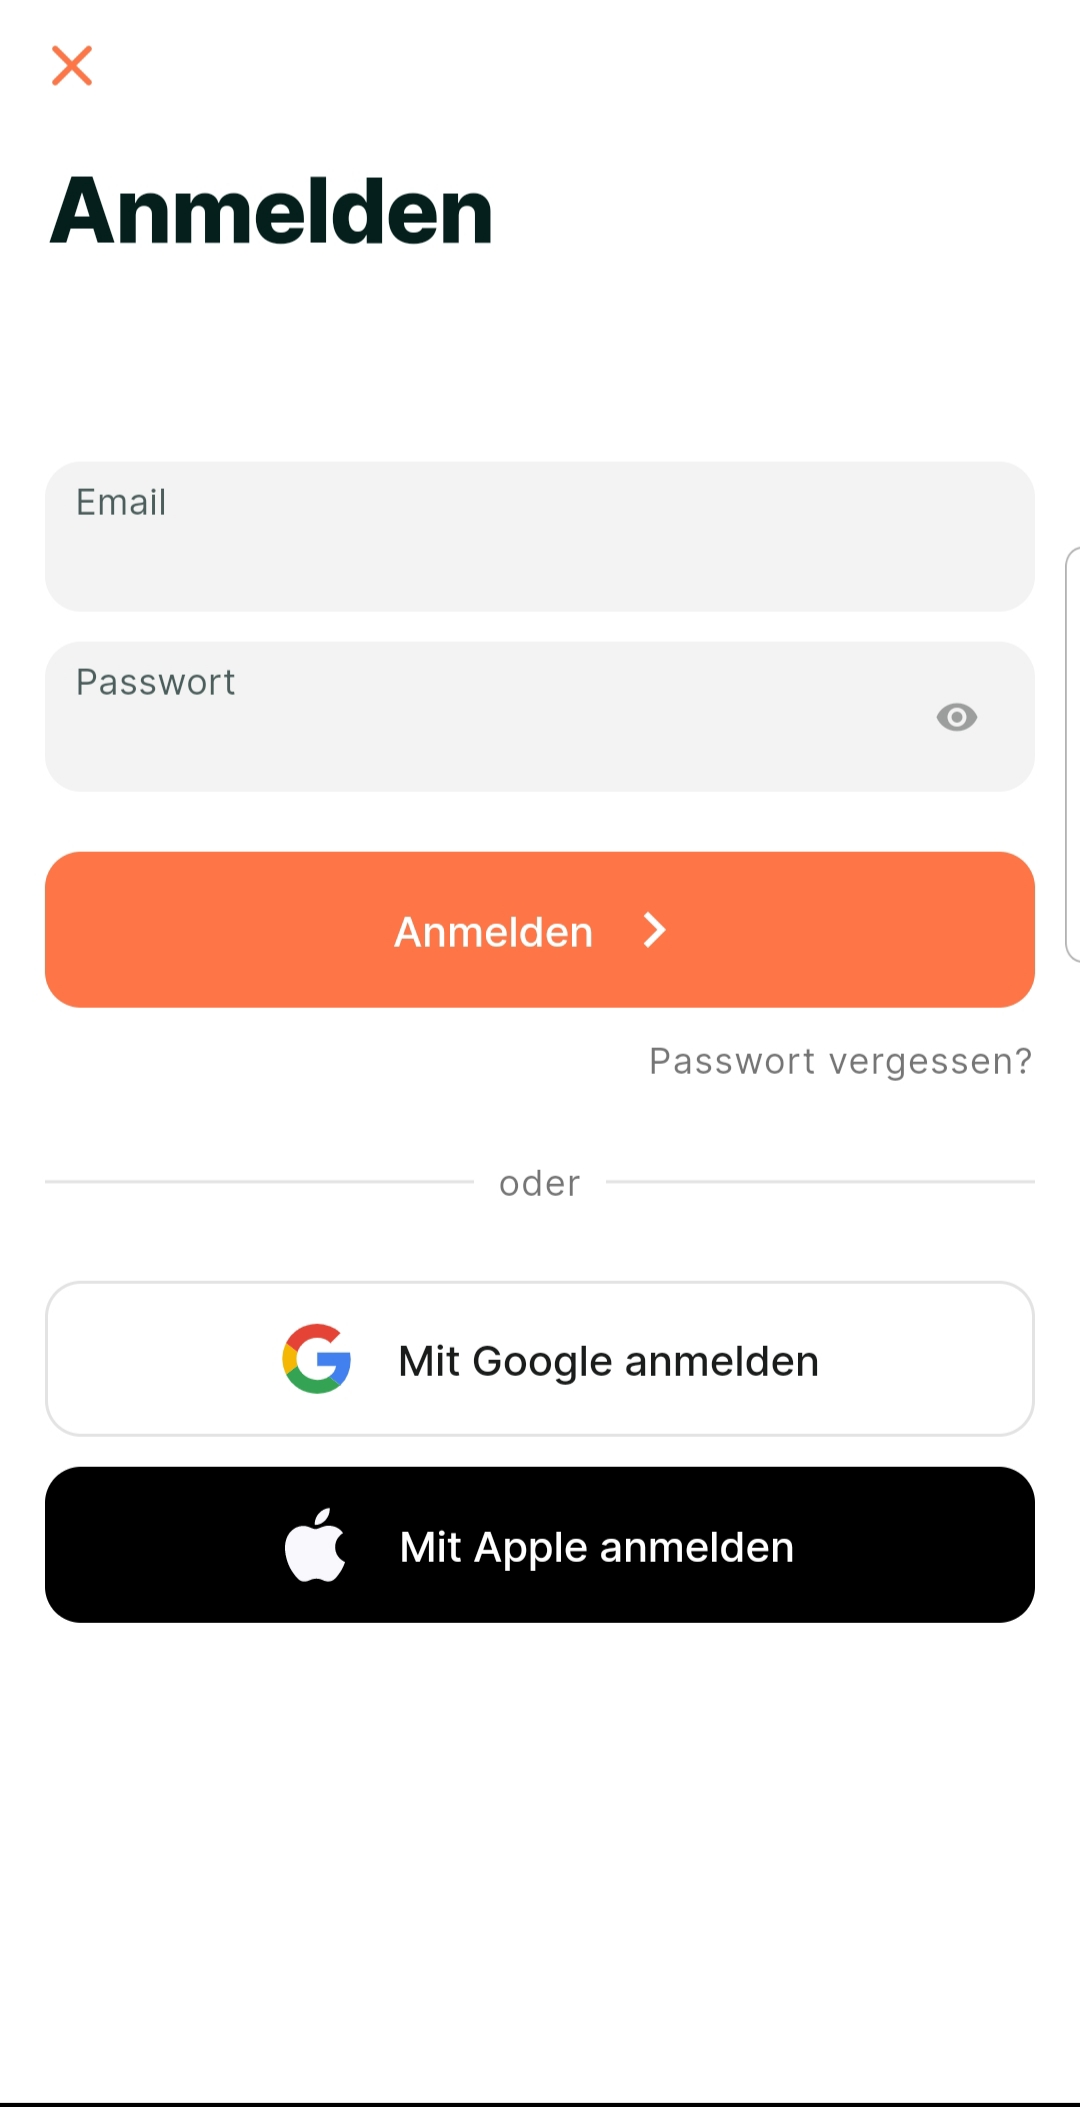
\includegraphics[width=0.3\textwidth]{pics/login-page.jpg}
  \caption{Login Ansicht auf der App}
  \label{fig:login-page}
\end{figure}

\subsubsection{Registrierungsprozess}
\setauthor{Sandin Habibovic}

\begin{figure}[h]
  \centering
  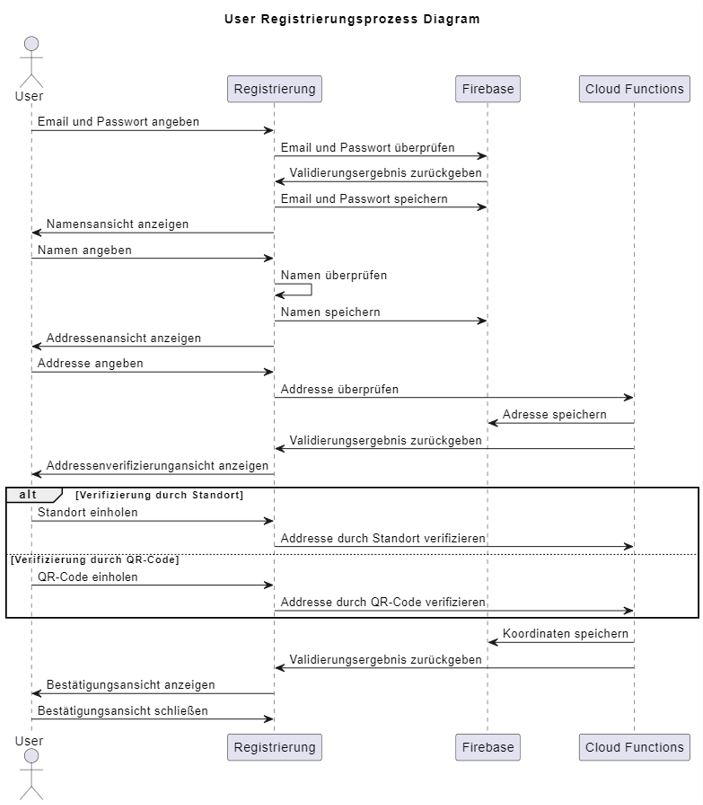
\includegraphics[width=0.9\textwidth]{pics/registration-sequence.JPG}
  \caption{Registrierungsprozess}
  \label{fig:registration-sequenze}
\end{figure}

Die Abbildung \ref{fig:registration-sequenze} repräsentiert ein Sequenzdiagram, welches den Registrierungsprozess für einen User veranschaulichen soll. Der Registrierungsprozess ist ein mehrstufiger Ablauf, wo sichergestellt werden soll, dass alle notwendigen Daten des Users erfasst und validiert werden, bevor die Registrierung abgeschlossen wird. Durch diesen Prozess wird gewährleistet, dass die erfassten Daten korrekt sind und dass nur verifizierte Benutzer Zugriff auf die Anwendung haben.
\\
Der Registrierungsprozess beginnt damit, dass der Benutzer aufgefordert wird, seine E-Mail-Adresse und ein Passwort anzugeben. Das Registrierungsformular leitet dann die E-Mail-Adresse und das Passwort Firebase weiter um es auf dessen Gültigkeit und Richtigkeit zu prüfen. Bei einer erfogreichen Prüfung werden die Daten eingespeichert und der User wird eingelogt.
\\
Nach überstehen des ersten Schrittes wird der nächste Schritt eingeleitet, die Namensansicht. Hier wird der Benutzer aufgefordert, seinen Namen und optional schon sein Profilbild anzugeben. Der Name wird dann ebenfalls vom Registrierungsformular auf Korrektheit und Vollständigkeit überprüft und im Firestore eingespeichert.
\\
Nachdem der Benutzer seinen Namen eingegeben hat, wird er zur Addressenansicht weitergeleitet, wo er aufgefordert wird, seine Adresse anzugeben. Wenn der User seine Adresse eingegeben hat, wird sie vom Registrierungsformular zu einer Cloud Function weitergeleitet und validiert. Falls sich die Addresse als eine korrekt Addresse erweist, wird sie direkt von der Cloud Function in den Firestore eingespeichert.
\\
Wenn die Adresse validiert wurde, wird der Benutzer aufgefordert, die Verifizierung seiner Adresse durchzuführen. Die Verifizierung kann durch zwei Methoden erfolgen. Entweder durch eine Überprüfung der Adresse anhand des Standortes oder durch eine Überprüfung der Adresse anhand eines gültigen QR-Codes. Das Registrierungsformular leitet den Standort oder QR-Code an eine Cloud Function weiter, die die Verifizierung übernimmt und bei erfolgreicher Verifizierung, die Koordinaten im Firestore einspeichert.
\\
Wenn die Verifizierung beendet wurde, ist der Registrierungsprozess abgeschlossen.
\\
Während des Registrierungsprozesses wird der User durch eine Authentifizierungsfunktion bereits eingeloggt, da eine Anmeldung für die Ausführung von Cloud Functions erforderlich ist. Wenn der Benutzer den Registrierungsprozess abbricht, werden alle bis zu diesem Punkt gesammelten Daten automatisch gelöscht, um die Datensicherheit und Privatsphäre des Users zu schützen. Wenn der User bei einem Schritt zurückgeht, werden die gespeicherten Daten von diesem Punkt zurückgesetzt, um sicherzustellen, dass nur korrekte Daten im Firestore gespeichert werden und dass keine ungültigen oder unvollständigen Daten gespeichert werden.
\\
Die Abbildung \ref{fig:registration-process} zeigt, wie der Registrierungs-Prozess in der App dargestellt wird.

\begin{figure}[h]
  \centering
  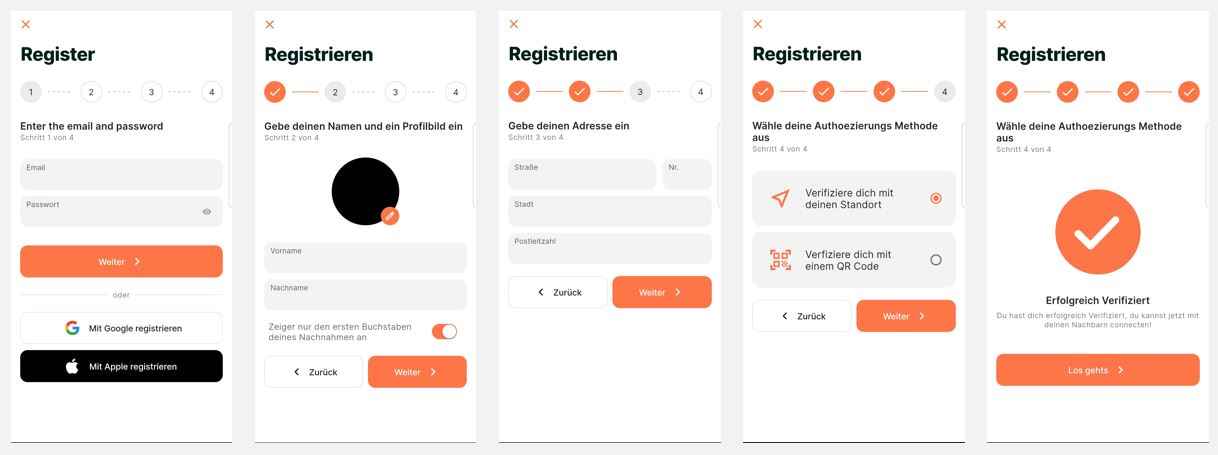
\includegraphics[width=\textwidth]{pics/registration-process.JPG}
  \caption{Registrierungsprozess in der App}
  \label{fig:registration-process}
\end{figure}

\paragraph{Google Barcode-Scanning ML Kit}\mbox{} \\
\setauthor{Martin Hausleitner}
In Anbetracht der Entscheidung, Einladungscodes mithilfe von QR-Codes zu implementieren, ist es erforderlich, einen QR-Code-Scanner während des Registrierungsprozesses zu integrieren. Um eine zuverlässige Benutzererfahrung zu gewährleisten, wurde das Google Barcode-Scanning ML Kit als bevorzugte Technologie ausgewählt. In internen Tests zeigte sich, dass dieses Kit eine hohe Genauigkeit und Zuverlässigkeit aufweist.
Die Integration des Scanners wurde mithilfe des Pakets \cite{mobile_scanner} mobile\_scanner realisiert, welches auf der Plattform pub.dev verfügbar ist. Dieses Paket ermöglicht eine einfache Implementierung und Anpassung an die individuellen Anforderungen des Projekts. Die Verwendung des ML-Kits trägt dazu bei, die Leistungsfähigkeit der Anwendung zu verbessern und die Benutzerzufriedenheit zu erhöhen.


Diagram
erklärung
screenshots

\subsection{Feed}
\setauthor{Sandin Habibovic}
Die Feed-Page stellt den zentralen Einstiegspunkt in der App dar und zeigt dem User alle aktuellen Beiträge und Updates aus der Nachbarschaft an.

\subsection{Beiträge}
\setauthor{Sandin Habibovic}
Beiträge sind das primäre Kommunikationsmittel auf der Plattform und erfordern vor der Veröffentlichung einen Titel, eine Beschreibung sowie eine Reichweite, unter der der Beitrag sichtbar sein soll. Zusätzlich können Bilder und Tags angehängt werden, um den Inhalt des Beitrags besser zu beschreiben und ihn leichter auffindbar zu machen.

\subsubsection{Kategorien}
\setauthor{Sandin Habibovic}
Um die Beiträge besser zuordnen zu können, müssen diese vor dem veröffentlichen einer bestimmten Kategorie zugeordnet werden. Diese Kategorien ermöglichen es den Usern, die Art Ihrer Anfrage ihm vorhinein besser zu spezifizieren und die Suche nach bestimmten Arten von Beiträgen zu vereinfachen. Bestimmte Kategorien werden weiters in Unterkategorien aufgeteilt, um die Art des Beitrags nochmals genauer zu spezifizieren.
\\
Es existieren folgende Kategorien bzw. Unterkategorien:

\begin{compactitem}
  \item Mitteilung
  \begin{compactitem}
    \item Frage
    \item Appell
    \item Warnung
    \item Empfehlung
    \item Gefunden
  \end{compactitem}
  \item Suche
  \begin{compactitem}
    \item Hilfe
    \item Verloren
  \end{compactitem}
  \item Ausleihen
  \item Event
\end{compactitem}

\textbf{Mitteilung:} Die Kategorie der Mitteilung dient dazu, die Nachbarn über bestimmte Ereignisse oder Nachrichten zu informieren oder sie um eine Meinung oder Empfehlung zu bitten.

\textbf{Suche:} Die Kategorie der Suche ermöglicht es den Nachbarn, im Falle von Hilfebedarf oder einem verlorenen Gegenstand, Kontakt mit ihren Nachbarn aufzunehmen.

\textbf{Ausleihen:} Die Kategorie der Ausleihens dient dazu die Nachbarn nach der Erlaubnis, sich ein bestimmtes Werkzeug oder Objekt ausborgen zu dürfen, zu bitten.

\textbf{Event:} Die Kategorie des Events dient dazu die Nachbarn auf eine bevorstehende Veranstaltung aufmerksam zu machen.

\\
Die Abbildung \ref{fig:categories} zeigt, wie die Auswahl der Kategorie bzw. Unterkategorie in der App dargestellt wird.

\begin{figure}[H]
  \centering
  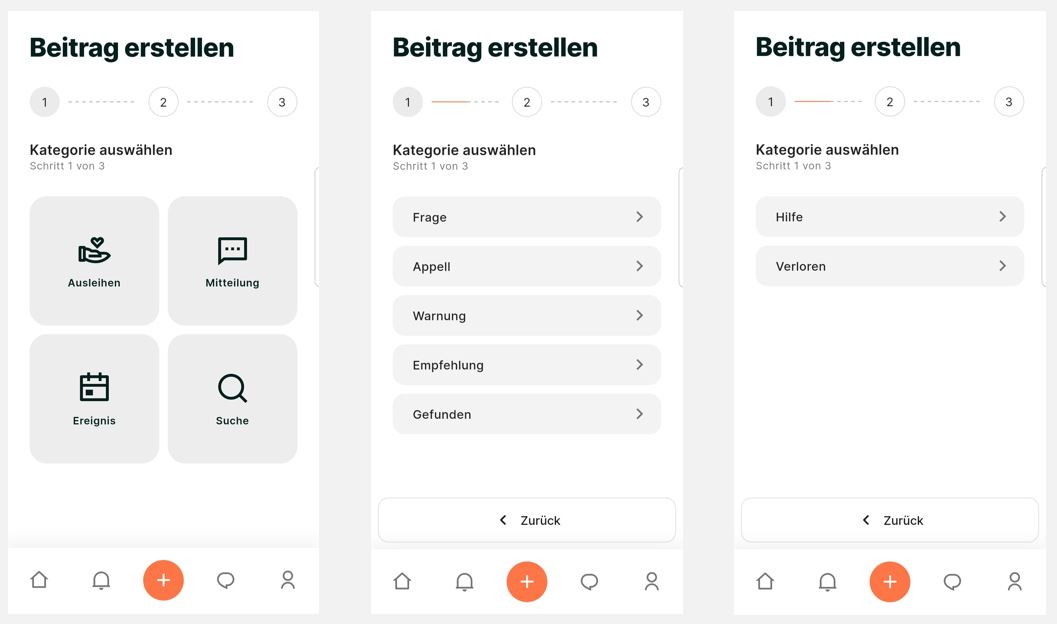
\includegraphics[width=\textwidth]{pics/categories.JPG}
  \caption{Auswahlansicht der Kategorien und Unterkategorien auf der App}
  \label{fig:categories}
\end{figure}


\subsubsection{Tags}
\setauthor{Sandin Habibovic}
Als Tag wird ein Schlüsselwort beschrieben, was man an ein Informationsgut anhängen kann, um es besser beschreiben zu können und/oder besser auffindbar zu machen. In der App werden Tags als eine Erweiterung der Kategorien verwendet, um es Usern zu ermöglichen Ihren Beitrag einem selbstdefinierten Typ zuzuordnen.

\subsubsection{Info}
\setauthor{Sandin Habibovic}
Jeder Beitrag hat eine eigene Sektion, wo wichtige Informationen über den Beitrag und den Ersteller des Beitrags angegeben werden, wie der Stadtteil, die ungefähre Entfernung zum gegebenen Nachbarn und das Erstelldatum des Beitrags.

\subsubsection{Kommentare}
\setauthor{Sandin Habibovic}
Die Kommentarfunktion ermöglicht es den Usern unter einem Beitrag Ihre Meinung, Feedback oder sonstiges zu hinterlassen.

\subsubsection{Beitrag oder Kommentar Melden}
\setauthor{Sandin Habibovic}
Um unangebrachte Beiträge oder Kommentare schnell zu identifizieren und auf diese schnell reagieren zu können, gibt es die Möglichkeit Beiträge oder Kommentare zu melden. Diese Meldungen können dann im Einzelnen überprüft werden. Fürs Melden muss ein Grund ausgewählt und eine genauere Beschreibung angegeben werden.
\\
Gründe fürs Melden eines Beitrags oder Kommentars:

\begin{compactitem}
  \item Unangebrachter Inhalt
  \item Belästigung
  \item Betrug
  \item Spam
  \item Sonstiges
\end{compactitem}

\subsubsection{Autovervollständigung
  mit Künstliche Intelligenz}
\setauthor{Martin Hausleitner}
\paragraph{GPT-3.5-turbo}\mbox{} \\


\begin{figure}[H]
  \centering
  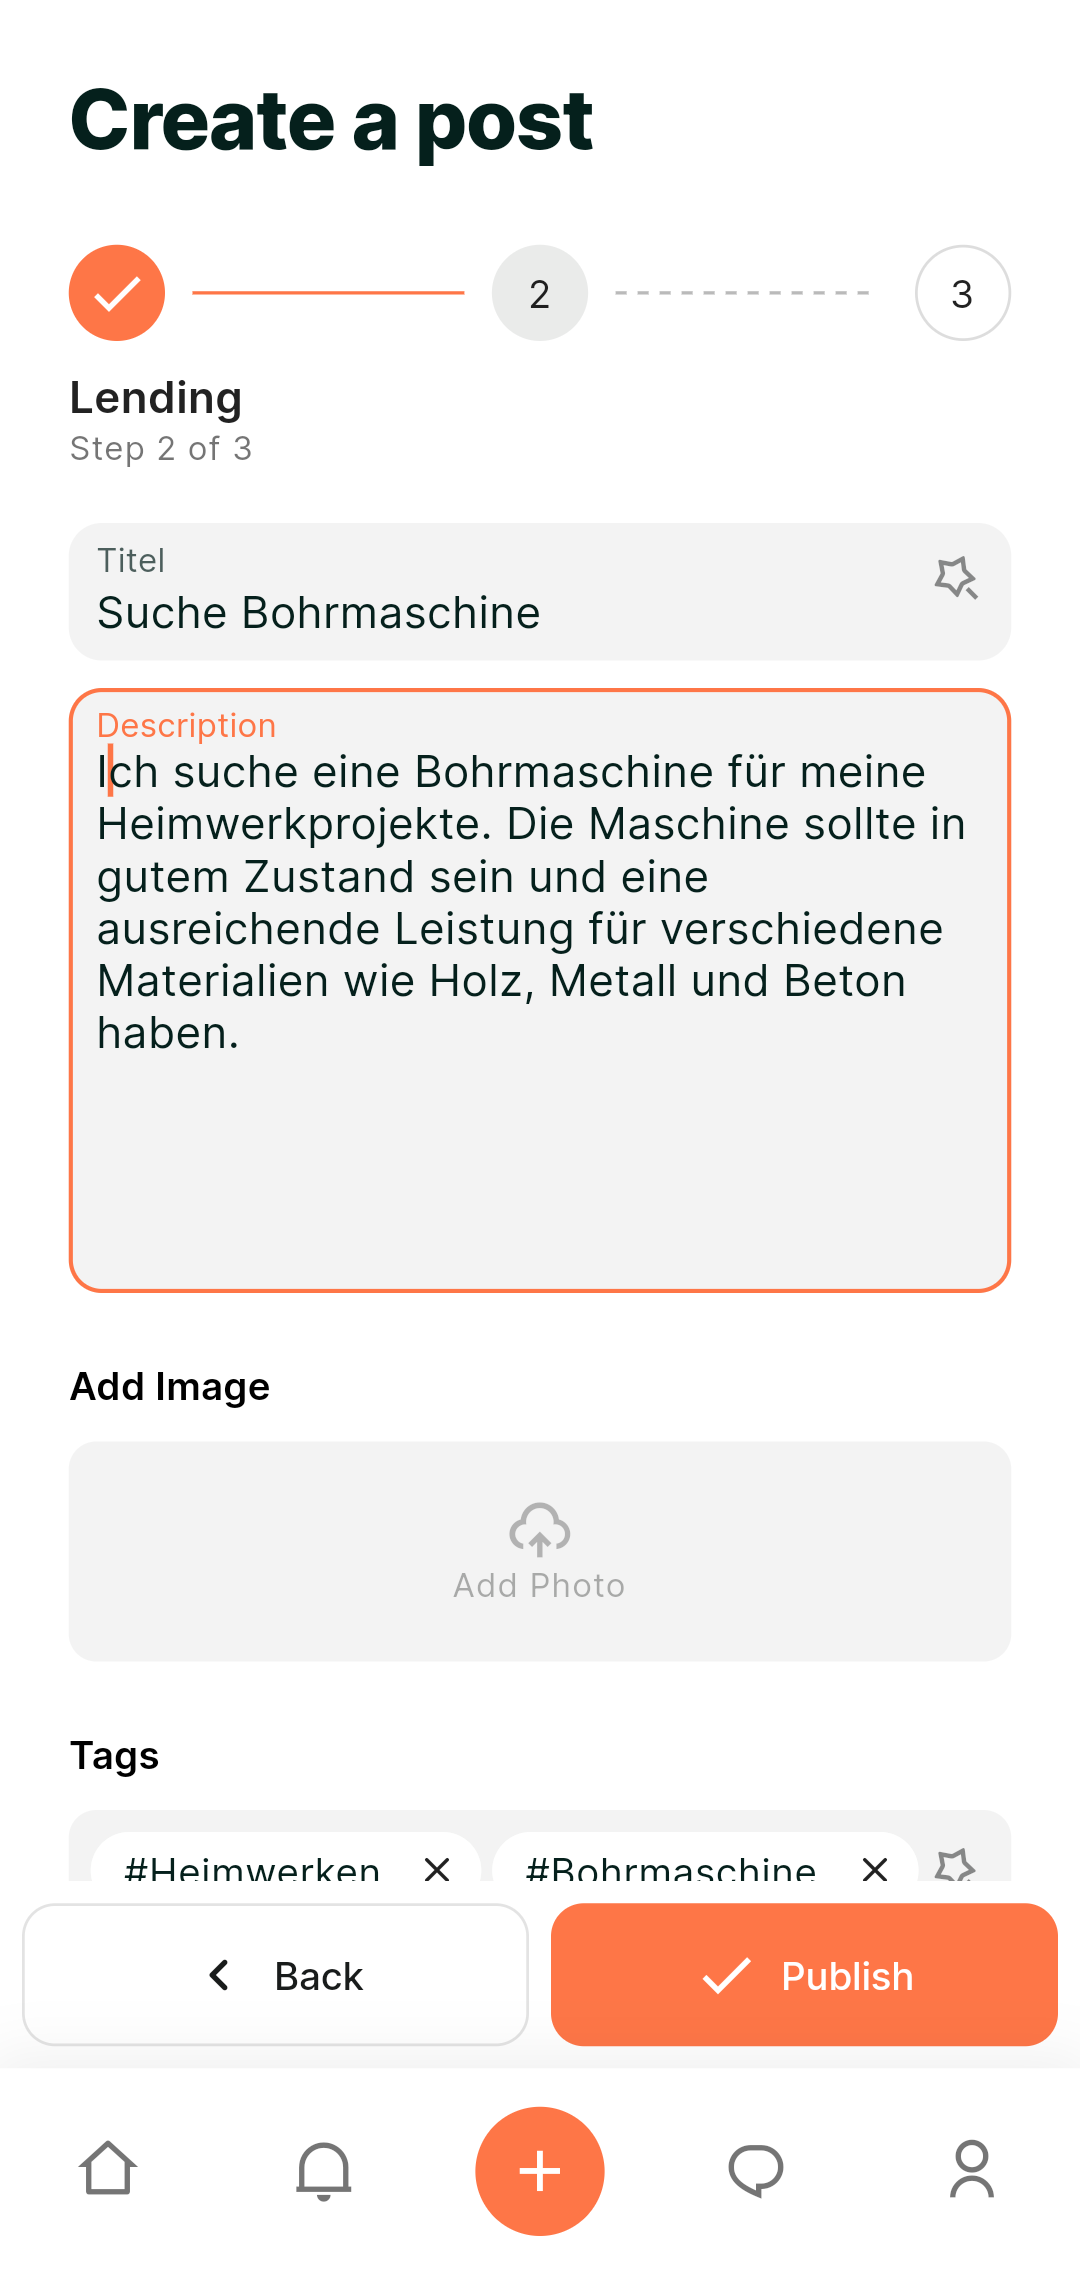
\includegraphics[width=0.3\textwidth]{pics/create-post.png}
  \caption{Schritt: 2 Beitrag erstellen}
  \label{fig:createpost}
\end{figure}


In jüngster Vergangenheit haben Fortschritte in der künstlichen Intelligenz (KI) dazu geführt, dass deren Implementierung in verschiedenen Produkten immer einfacher wird. Das Entwicklerteam hat daher beschlossen, auch in Nochba eine vereinfachte Implementierung durchzuführen. Mit der Veröffentlichung der GPT-3.5-turbo API von OpenAI wurde diese unmittelbar in Nochba integriert. Wie in der Abbildung \ref{fig:createpost} ersichtlich, befindet sich im Titelfeld ein Zauberstab-Symbol in der rechten oberen Ecke. Bei einem Klick darauf wird eine API-Anfrage an OpenAI gesendet. Um einen Titel basierend auf der Beschreibung zu erstellen, wird folgender Prompt benötigt:
\begin{verbatim}
beschreibung{ ${widget.descriptionController!.text} } passender Titel:
\end{verbatim}

Die KI liefert stets zuverlässig einen passenden Titel.

Ein ähnlicher Ansatz wurde auch für die Tags verfolgt. Der Titel und die Beschreibung wurden als Kontext für die KI verwendet. Nach mehreren Versuchen wurde der passende Prompt gefunden, da die KI-Ausgabe zunächst inkonsistent war und nicht erfolgreich in Tags umgewandelt werden konnte. Mit dem folgenden Prompt wurde der Output zuverlässiger:

\begin{verbatim}
titel{ $ {widget.titleController!.text }  } beschreibung { ${widget.descriptionController!.text }  } json hashtags richtige sprache: ["#
\end{verbatim}


Die letzten Zeichen ["\# wurden absichtlich gewählt, da die
KI-Ausgabe manchmal mit oder ohne \# geschrieben wurde, was
das Parsen der Tags erschwerte. Durch die Klammer und das \#
werden nun zuverlässig im JSON-Format und Tags mit \#
erstellt.

Der folgende Code \ref{lst:parseTags} wird verwendet, um die Tags aus der KI-Ausgabe zu parsen und sie anschließend dem TagsController zu übergeben:

\begin{lstlisting}[language=Java,caption=parseTags von 
  KI output,label=lst:parseTags]  
  
  List<String> parseTags(String chatOutput) {
    RegExp regExp = RegExp(r'(?<=#)[\p{Letter}]+', unicode: true);
    Iterable<RegExpMatch> matches = regExp.allMatches(chatOutput);
    List<String> tags = [];

    for (RegExpMatch match in matches) {
      String tag = match.group(0)!;
      tags.add(tag);
    }

    print(tags.toString());

    return tags;
  }
    
\end{lstlisting}


Da die Nutzung der KI kostenintensiv sein kann, wenn mehr Benutzer sie verwenden, ist die Nutzung auf maximal zwei Anfragen pro Benutzer für Titel- oder Tag-Generierung begrenzt. Zukünftig ist geplant, das System durch ein Nochba AI-Abo mit unbegrenzten Anfragen zu monetarisieren.

\subsubsection{Übersetzung mit Maschine Learning}

\paragraph{Google Translation ML Kit}\mbox{} \\

Für die Übersetzung von Beiträgen vom Deutschen ins Englische wurde eine kosteneffiziente Methode gesucht, um Kosten zu minimieren. Zunächst wurden bekannte Übersetzungs-APIs analysiert, aber dann stieß der Entwickler auf das Google ML Kit, welches 50 Sprachen übersetzen kann. Bemerkenswert ist, dass ein Sprachpaket etwa 5 MB umfasst und auch offline verwendet werden kann. Beim Start der App werden das deutsche und englische Sprachmodell heruntergeladen. Um einen Beitrag zu übersetzen, muss der Benutzer länger auf den Beitrag klicken, um die Übersetzung zu starten.



\paragraph{Google Language identification ML Kit}\mbox{} \\

Um eine Sprache überhaupt übersetzen zu können, benötigt man ein Werkzeug zur Spracherkennung. In dieser App wird das Google Spracherkennungs-ML-Kit verwendet. Bevor der Benutzer einen Beitrag übersetzen möchte, werden die Beschreibung und der Titel an das maschinelle Lernmodell gesendet, um die erkannte Sprache dem Übersetzungs-ML-Kit zu übergeben und eine Übersetzung durchzuführen.


\subsection{Filter}
\setauthor{Sandin Habibovic}
Der Filter bietet die Option die Beiträge nach bestimmten Kriterien zu filtern und die Suche nach bestimmten Beiträge zu vereinfachen. Der Filter unterteilt sich in einen Menüfilter und Hauptfilter.

\subsubsection{Menüfilter}
\setauthor{Sandin Habibovic}

Die Ansicht vom Menüfilter befindet sich direkt über den Beiträgen und ermöglicht eine schnelle Filterung nach einzig allein den Hauptkategorien.
\\
Die folgende Abbildung \ref{fig:menu-filter} zeigt, wie der Menüfilter in der App dargestellt wird.

\begin{figure}[h]
  \centering
  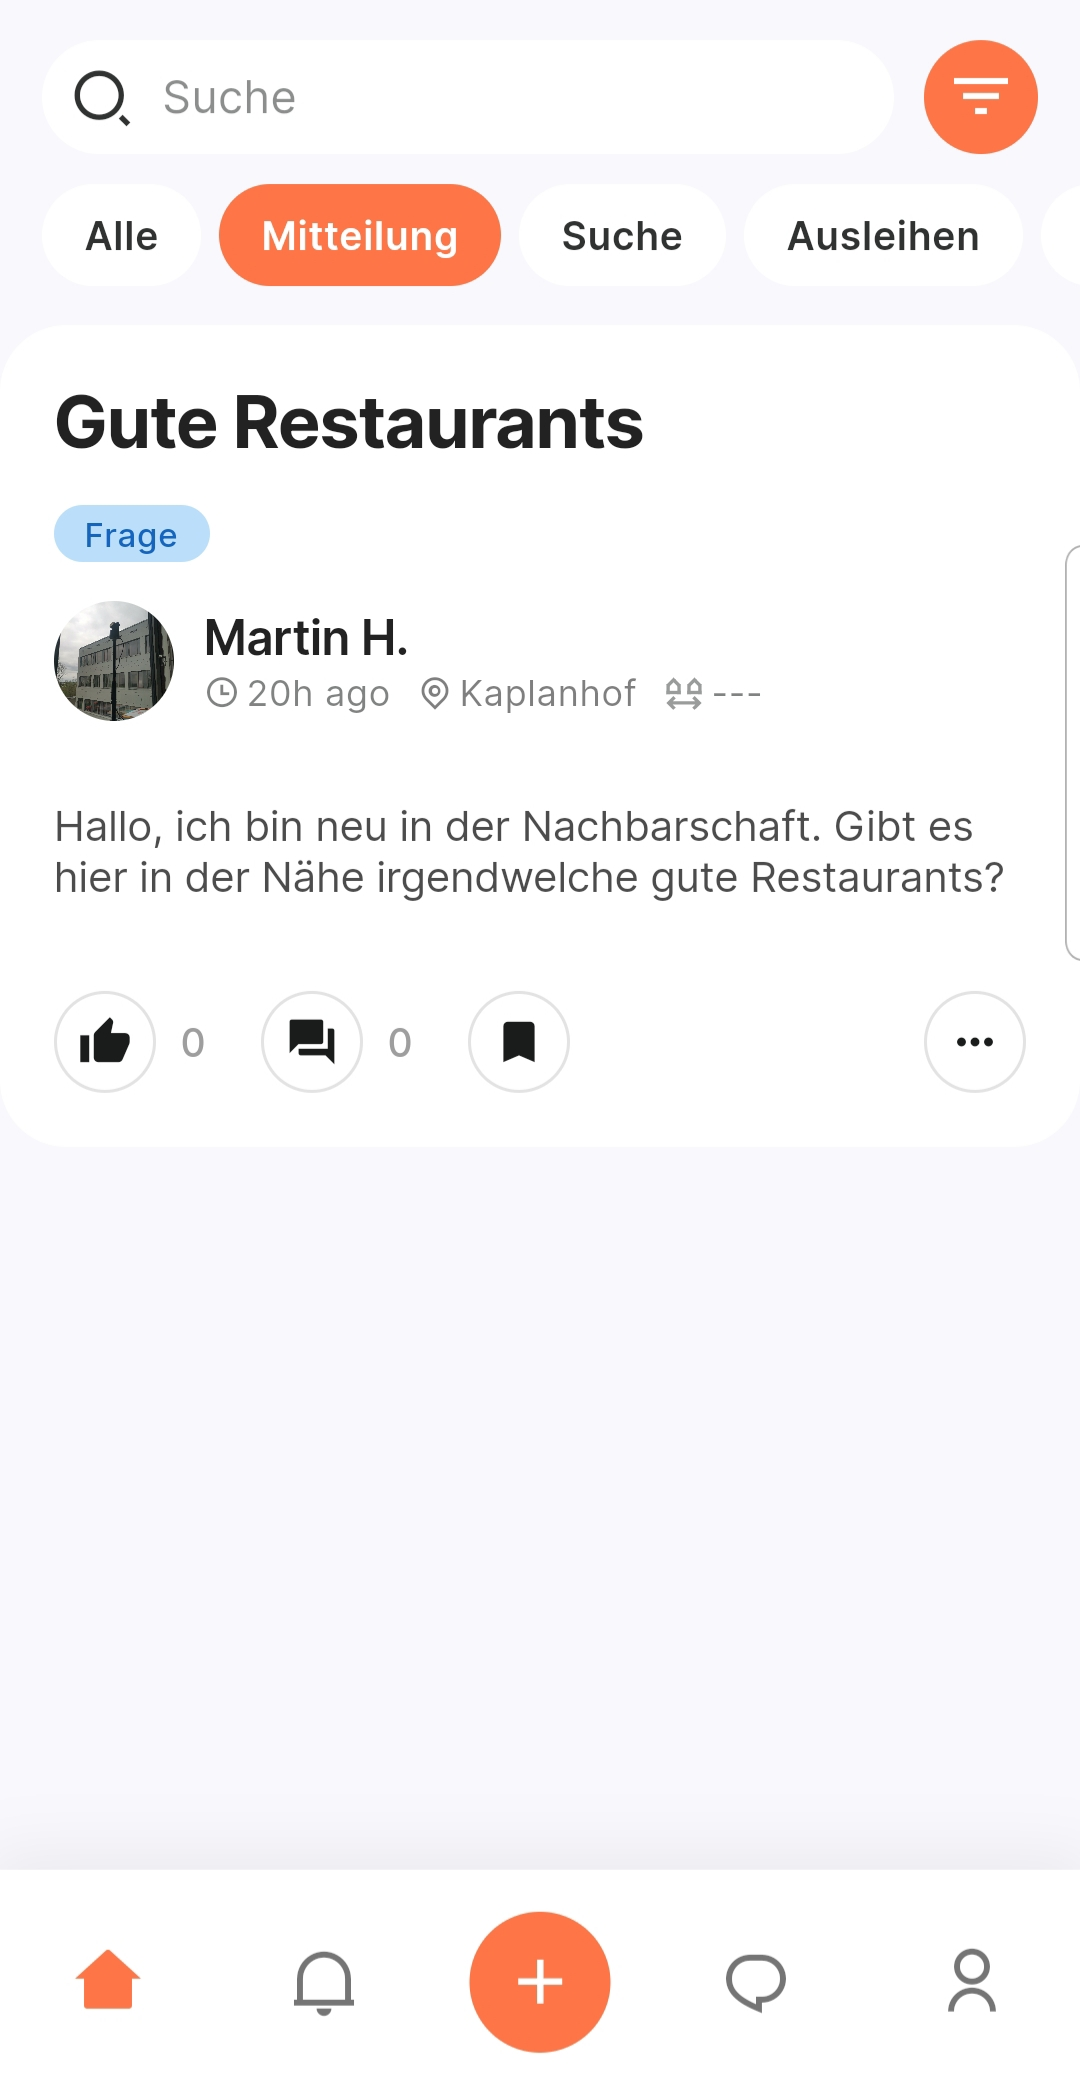
\includegraphics[width=0.3\textwidth]{pics/menu-filter.jpg}
  \caption{Menüfilteransicht auf der App}
  \label{fig:menu-filter}
\end{figure}

\subsubsection{Hauptfilter}
\setauthor{Sandin Habibovic}

Die Ansicht vom Hauptfilter taucht erst nach dem Antippen vom Filtersymbol auf und beinhaltet eine größere Auswahl an Filteroptionen. Darunter zählt neben dem Filtern nach Hauptkategorien auch die zusätzliche Möglichkeit genauer nach Unterkategorien zu suchen. Außerdem besteht auch die Option die Beiträge nach Datum oder Likes zu sortieren oder die Beiträge aufsteigend oder absteigend zu ordnen.
\\
Die folgende Abbildung \ref{fig:main-filter} zeigt, wie der Hauptfilter in der App dargestellt wird.

\begin{figure}[h]
  \centering
  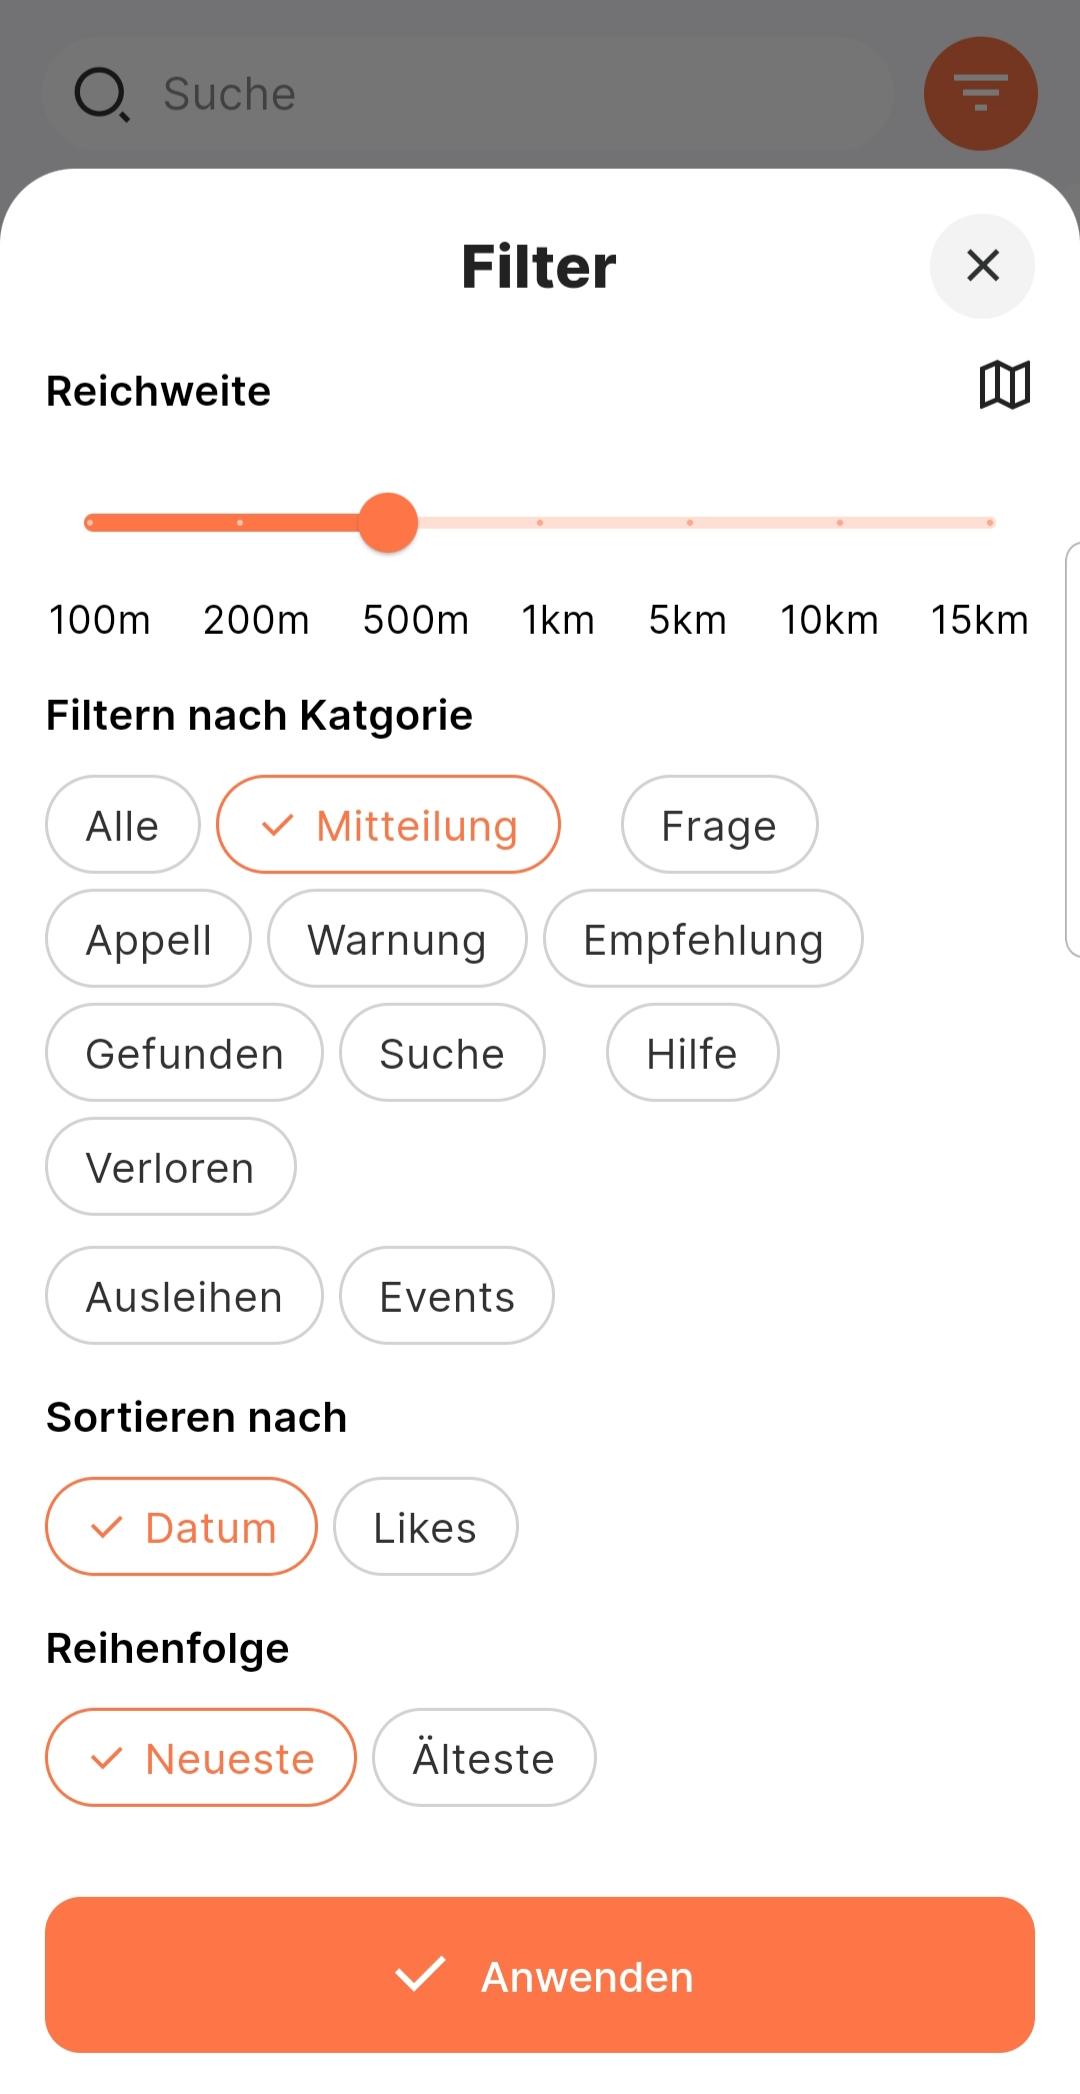
\includegraphics[width=0.3\textwidth]{pics/main-filter.jpg}
  \caption{Hauptfilteransicht auf der App}
  \label{fig:main-filter}
\end{figure}

\subsubsection{Filtern der Reichweite}
\setauthor{Sandin Habibovic}

Die wichtigste Filterkomponente ist der Range-Slider, womit die Beiträge nach der Reichweite gefiltert werden können, da die Entfernung zum Nachbarn eine der wichtigsten Entscheidungsfaktoren zum Antworten auf einem Beitrag ist.
\\
Die folgende Abbildung \ref{fig:range-filter} zeigt, wie der Reichweitenfilter in der App dargestellt wird.

\begin{figure}[h]
  \centering
  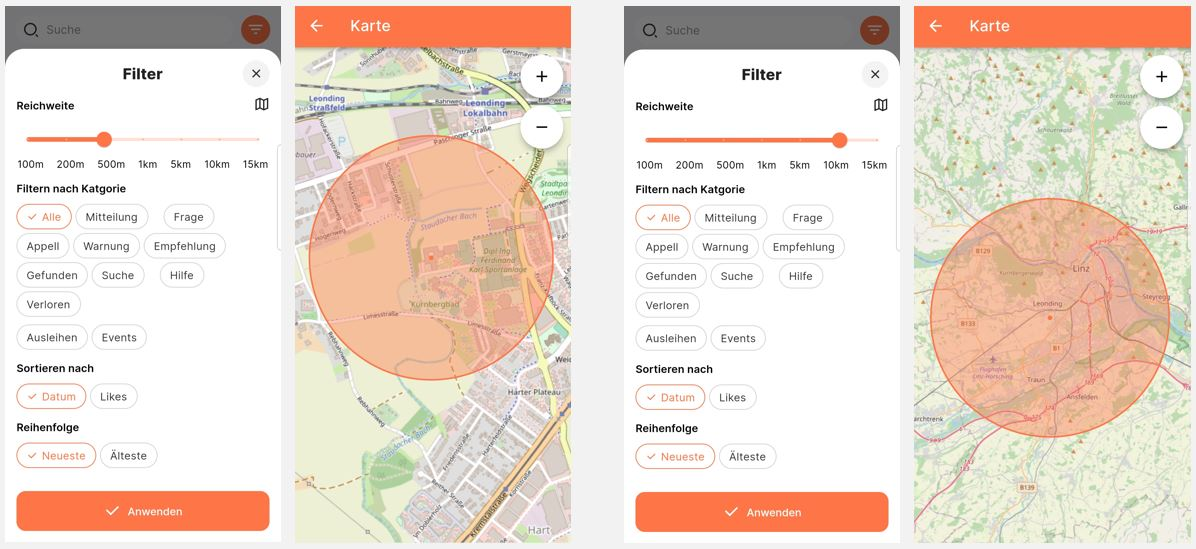
\includegraphics[width=\textwidth]{pics/range-filter.JPG}
  \caption{Filtern der Reichweite}
  \label{fig:range-filter}
\end{figure}

\subsection{Suche}

Eine gut umgesetzte Suchfunktion in einer Social-Media-App stellt eine wichtige Funktion für den Aufbau einer lokalen Gemeinschaft und die gemeinsame Nutzung von Ressourcen dar. Durch die Verbesserung der Entdeckungsmöglichkeiten und der Personalisierung kann die Suchfunktion erheblich zum Erfolg der Plattform beitragen und die häufige Nutzung durch die Community-Mitglieder fördern.

Eine Suchfunktion kann auf folgende Weise zum Erfolg einer Social Media App beitragen:

\begin{itemize}
  \item \textbf{Entdeckungsmöglichkeit:}
        \begin{itemize}
          \item {Eine robuste Suchfunktion ermöglicht es den Nutzern, problemlos wichtige Inhalte, Personen und Ressourcen innerhalb ihrer lokalen Gemeinschaft zu finden. Dies hilft bei der Entdeckung neuer Verbindungen und Veranstaltungen und trägt letztlich zur Verstärkung der lokalen Gemeinschaft und zur Förderung des sozialen Engagements bei.}
        \end{itemize}
  \item \textbf{Personalisierung:}
        \begin{itemize}
          \item {Die Nutzer können die Suchfunktion nutzen, um Inhalte zu finden, die auf ihre individuellen Interessen und Bedürfnisse zugeschnitten sind. Diese Personalisierung führt zu einer höheren Kundenzufriedenheit, da sich die Nutzer stärker mit der Plattform assoziiert fühlen.}
        \end{itemize}
  \item \textbf{Zeiteffizienz:}
        \begin{itemize}
          \item {Eine Suchfunktion ermöglicht es den Benutzern, die gesuchten Informationen schnell und effizient zu finden. Das spart Zeit und Mühe, macht die Plattform attraktiver und erhöht die Wahrscheinlichkeit, dass sie häufig genutzt wird.}
        \end{itemize}
\end{itemize}

\subsection{Typesense}
\setauthor{Arsham Edalatkhah}
Das Nochba-Team versuchte ursprünglich, Typesense für die Suchfunktionalität zu verwenden, da es sich um eine schnelle, fehlertolerante Suchmaschine handelt, die für sofortige Suchvorgänge optimiert ist. Aufgrund der unvollständigen Dokumentation hatte das Team jedoch Schwierigkeiten, Typesense in die Flutter-Applikation zu implementieren. Arsham Edalatkhah versuchte, die Typesense-Entwickler um Unterstützung zu bitten, aber dieser Schritt war sehr zeitaufwändig.

Typesense war aus mehreren Gründen eine ausgezeichnete Wahl für das Nochba-Team:

\begin{itemize}
  \item \textbf{Geschwindigkeit:}
        \begin{itemize}
          \item {Typesense ist darauf optimiert, Suchergebnisse schnell zu liefern und so ein flüssiges und reibungsloses Sucherlebnis zu ermöglichen.}
        \end{itemize}
  \item \textbf{Tippfehler-Toleranz:}
        \begin{itemize}
          \item {Typesense kann mit Tippfehlern umgehen und trotzdem relevante Suchergebnisse liefern. Dies ist eine wichtige Funktion für eine Suchmaschine, da Nutzer beim Tippen oft Fehler machen. Durch die Berücksichtigung dieser Fehler stellt Typesense sicher, dass die Nutzer auch dann korrekte Ergebnisse erhalten, wenn ihre Anfrage Tippfehler enthält.}
        \end{itemize}
  \item \textbf{Tippfehler-Toleranz:}
        \begin{itemize}
          \item {Typesense kann mit Tippfehlern umgehen und trotzdem relevante Suchergebnisse liefern. Dies ist eine wichtige Funktion für eine Suchmaschine, da Nutzer beim Tippen oft Fehler machen. Durch die Berücksichtigung dieser Fehler stellt Typesense sicher, dass die Nutzer auch dann korrekte Ergebnisse erhalten, wenn ihre Anfrage Tippfehler enthält.}
        \end{itemize}
\end{itemize}

In diesem Fall entschied sich das Nochba-Team, zu Algolia zu wechseln, das ähnliche Funktionen wie Typesense bietet. Beide Suchmaschinen bieten schnelle, typentolerante und anpassbare Suchergebnisse. Die Entscheidung für Algolia ermöglichte es dem Team, die mit Typesense aufgetretenen Herausforderungen bei der Implementierung zu überwinden und eine effektive Suchfunktionalität innerhalb der App bereitzustellen.

\subsection{Algolia}
\setauthor{Arsham Edalatkhah}

Die finale Entscheidung des Nochba-Teams fiel auf die Algolia-Suche, da sowohl Typesense als auch Algolia den gleichen Feature-Set für Suchfunktionen bieten. Ein bemerkenswerter Unterschied zwischen beiden ist, dass Algolia eine umfangreichere Dokumentation und Unterstützung bietet, was es für Entwickler einfacher macht, die Suchfunktion zu implementieren und in ihre Anwendung zu integrieren.

Das Team Nochba hat die folgenden Schritte zur Einrichtung und Installation der Algolia-Suche durchgeführt:

\begin{itemize}
  \item {Zusätzlich wurde das Algolia-Paket als 'Abhängigkeit' in der Datei pubspec.yaml eingetragen.}
  \item {'Flutter packages get' wurde ausgeführt, um die Abhängigkeit zu installieren.
        Import des Algolia-Pakets in die entsprechende Dart-Datei.}
  \item {Initialisierung einer Algolia-Instanz durch Angabe der Applikations-ID und des API-Keys.}
  \item {Konfiguration der durchsuchbaren Kategorien durch die Einstellung der 'searchableAttributes' im Algolia-Dashboard, die 'description', 'title', 'tags' und 'category' umfassen.}
\end{itemize}

\subsubsection{Firestore Sync}

\subsubsection{Testbenutzer für Entwickler}
\setauthor{Arsham Edalatkhah}

Das Team Nochba hat beschlossen, auf der Registrierungs-/Anmeldeseite eine weitere Funktion speziell für die Entwickler einzurichten. Diese Option ermöglicht die sofortige Erstellung eines 'Testbenutzers'. Nach dem Anklicken der Schaltfläche wird der Testbenutzer automatisch registriert und verifiziert. Der wesentliche Grund für die Entscheidung von Team Nochba war die Vereinfachung des Entwicklungsvorgangs, da sich das Team nicht mehr jedes Mal neu anmelden oder registrieren muss, wenn es die Applikation während der Entwicklung erneut geladen wird. Dieser Ansatz spart viel Zeit und beschleunigt den Entwicklungsprozess.

Testbenutzer oder Mock-User stehen in der Entwicklungsversion ausschließlich den Developern zur Verfügung, während sie im Release-Modus für die Tester nicht zugänglich sind. Durch die Trennung der Testbenutzer von den tatsächlichen Benutzern stellt das Team Nochba sicher, dass die Entwicklungsumgebung von der Testumgebung getrennt bleibt, um unbeabsichtigte Folgen oder Störungen des Testprozesses zu vermeiden. Diese Strategie ermöglicht es dem Team, eine hohe Softwarequalität beizubehalten und stellt sicher, dass das finale Produkt zuverlässig, sicher und effizient ist.


\subsection{Chat}
\setauthor{Arsham Edalatkhah}

Für die Nutzer einer Nachbarschaftshilfe-App, die sich auf den Aufbau von Gemeinschaften und die gemeinsame Nutzung von Ressourcen spezialisiert hat, bedeutet die Möglichkeit, miteinander zu chatten, dass die Nutzer leicht mit ihren Nachbarn in Kontakt treten, Ideen austauschen, Ressourcen gemeinsam nutzen und stärkere Beziehungen innerhalb ihrer Gemeinschaft aufbauen können. So können sie sich über lokale Geschehnisse auf dem Laufenden halten und haben eine Plattform, um Probleme in der Gemeinschaft zu besprechen und zu lösen.

Die Studie 'Core Networks, Social Isolation, and New Media: Internet and Mobile Phone Use, Network Size and Diversity' von Keith Hampton und anderen aus dem Jahr 2011 (Quelle: \cite{hampton2011core} ) untersuchte den Zusammenhang zwischen der Nutzung von Internet und Mobiltelefonen und der Größe und Diversität sozialer Netzwerke. Obwohl diese Studie nicht speziell Nachbarschafts-Apps untersuchte, zeigt sie den potenziellen Nutzen von Online-Netzwerken für den Aufbau von Gemeinschaften und die Stärkung von Beziehungen.

Die Möglichkeit, in einer Nachbarschafts-App wie Nochba zu chatten, kann dazu beitragen, den Austausch von Ideen und Ressourcen unter den Nutzern zu erleichtern, lokale Geschehnisse zu verfolgen und Probleme in der Gemeinschaft zu lösen. Diese Chat-Funktion kann daher dazu beitragen, den Aufbau von Gemeinschaften und sozialem Engagement zu fördern, wie es auch von den Entwicklern von Nochba betont wird.

Aus Sicht der Entwickler ist die Möglichkeit, mit anderen Nutzern zu chatten, eine wichtige Funktion der App, die den Aufbau von Gemeinschaften und das soziale Engagement fördert. Das Nochba-Team ist sich bewusst, wie wichtig es ist, starke Community-Verbindungen zu fördern, und ist der Ansicht, dass die Möglichkeit der Kommunikation zwischen den Nutzern eine entscheidende Rolle bei der Erreichung dieses Ziels spielt. Durch die Bereitstellung einer Chat-Funktion ist das Nochba-Team in der Lage, eine umfassendere und interaktivere Plattform zu schaffen, die die Benutzer dazu ermutigt, sich untereinander auszutauschen und ein stärkeres Gemeinschaftsgefühl zu entwickeln.

Gemäß der Studie 'Neighborly Networks: A Study of Online Community Life' von Keith N. Hampton und anderen werden im Folgenden einige weitere Gründe aufgeführt, warum die Möglichkeit, in einer Social-Media-App für die Nachbarschaft miteinander zu chatten, von Vorteil sein kann:

\begin{itemize}
  \item \textbf{Für die Nutzer:}
        \begin{itemize}
          \item {Sie können ihre Nachbarn um Empfehlungen für nahe gelegene Dienstleistungen oder Geschäfte bitten.}
          \item {Sie können lokale Events oder Treffen organisieren und die Details mit anderen interessierten Mitgliedern der Nachbarschaft besprechen.}
          \item {Straßensperrungen, die sich auf die Anwohner auswirken können.}
          \item {Sie bietet eine Plattform für den Austausch von Neuigkeiten aus der Umgebung, wie beispielsweise aktuelle Informationen über Bauarbeiten.}
          \item {Es kann das Gefühl der Sicherheit fördern, da die Nachbarn im Notfall schnell und einfach miteinander in Kontakt treten können.}
          \item {Es kann dazu beitragen, ein stärkeres Gemeinschaftsgefühl zu bilden, da die Nutzer Geschichten, Erinnerungen und Erfahrungen miteinander teilen können.}
        \end{itemize}
\end{itemize}

\begin{itemize}
  \item \textbf{Für Entwickler:}
        \begin{itemize}
          \item {Das Engagement der Nutzer und die Zeit, die sie mit der App verbringen, können gesteigert werden, da die Nutzer mehr Zeit mit dem Chatten verbringen können.}
          \item {Es kann zu mehr Inhalten führen, die von Nutzern erstellt werden, wie beispielsweise Fotos oder Informationen zu Events, die in der App geteilt werden können.}
          \item {Sie kann wichtige Daten über das Verhalten und die Vorlieben der Nutzer liefern, die in künftige Entwicklungsentscheidungen einfließen können.}
          \item {Es kann die App von der übrigen Konkurrenz abheben und sie für potenzielle Nutzer attraktiver machen.}
          \item {Sie kann dazu beitragen, dass Benutzer, die die gemeinschaftsbildenden Aspekte der App zu schätzen wissen, dem Hersteller und seinen Produkten vertrauen und für sie eintreten.}
        \end{itemize}
\end{itemize}

Vergleich 'Flyer Chat' und 'Stream Chat Flutter'

Es gibt ein Flutter-Chatpaket namens 'Flyer Chat', das momentan das am besten bewertete Chatpaket auf dem Gebiet ist. Ein weiteres hoch geschätztes Chat-Paket für Flutter-Applikationen ist 'Stream Chat Flutter'.

'Flyer Chat' bietet eine Chat-Benutzeroberfläche und unterstützt die Grundfunktionalität, indem es Entwicklern vorgefertigte Chat-UI-Komponenten wie Chat-Bubbles, Eingabefelder und Nachrichtenlisten zur Verfügung stellt. Dieses Paket ermöglicht es Entwicklern, auf einfache und schnelle Weise Chat-Funktionen in ihre Applikationen zu implementieren und sie an das Design der App anzupassen. Darüber hinaus ist 'Flyer Chat' so gestaltet, dass es reibungslos mit gängigen Backend-Diensten für die Speicherung und den Abruf von Chat-Daten zusammenarbeitet und bietet eine übersichtliche Dokumentation, Code-Beispiele und Tutorials, um die Benutzerfreundlichkeit zu unterstützen.

'Stream Chat Flutter' hingegen ist ein SDK, mit dem Entwickler Echtzeit-Chat-Anwendungen für Flutter erstellen können. Es bietet Funktionen wie integrierte UI-Komponenten, Offline-Unterstützung, anpassbare Themen und Unterstützung für mehrere Plattformen, einschließlich Android, iOS und Web.

Für das Team Nochba war es aus folgenden Gründen eine bessere Idee, das 'Flyer Chat'-Paket zu verwenden:

\begin{itemize}
  \item \textbf{Integration:}
        \begin{itemize}
          \item {'Flyer Chat' bietet eine nahezu reibungslose Installation in bestehende Flutter-Applikationen, was eine unkomplizierte Erfahrung für Entwickler darstellt.}
        \end{itemize}
  \item \textbf{Funktionsumfang:}
        \begin{itemize}
          \item {'Flyer Chat' verfügt über einen umfassenden Feature-Set, das ein optimales Verhältnis zwischen häufig verwendeten Chat-Funktionen und innovativen, individuellen Eigenschaften ermöglicht.}
        \end{itemize}
  \item \textbf{Leistung:}
        \begin{itemize}
          \item {Der 'Flyer Chat' ist für verschiedene Plattformen optimiert, um ein flüssiges Benutzererlebnis zu ermöglichen, ohne die Leistung der App zu verringern.}
        \end{itemize}
  \item \textbf{Dokumentation und Unterstützung:}
        \begin{itemize}
          \item {Mit gut dokumentierten Materialien und einer starken Community macht es 'Flyer Chat' den Entwicklern besonders einfach, Lösungen für allgemeine Probleme zu finden und Anpassungen vorzunehmen.}
        \end{itemize}
\end{itemize}

Software-Engineering mit komponentenorientierter Entwicklung

Laut dem 1998 veröffentlichten Fachbuch (Quelle: \cite{szyperski-component} )'Component-Oriented Programming' von Clemens Szyperski können Komponenten unabhängig voneinander entwickelt, getestet und gewartet werden, was mehrere Vorteile bietet:

\begin{itemize}
  \item \textbf{Wiederverwendbarkeit:}
        \begin{itemize}
          \item {Komponenten können über mehrere Applikationen hinweg wiederverwendet werden, was die Entwicklungszeit und den Aufwand verkürzt.}
        \end{itemize}
  \item \textbf{Wartbarkeit:}
        \begin{itemize}
          \item {Gut definierte Grenzen machen es viel bequemer, Probleme in einer bestimmten Komponente zu erkennen und zu beheben, ohne den Rest der Applikation zu beeinträchtigen.}
        \end{itemize}
  \item \textbf{Skalierbarkeit:}
        \begin{itemize}
          \item {Anwendungen können durch den Import oder die Substitution von Komponenten ohne größere Anpassungen leicht skaliert werden.}
        \end{itemize}
  \item \textbf{Flexibel:}
        \begin{itemize}
          \item {Der modulare Aufbau ermöglicht eine einfache Anpassung an sich verändernde Anforderungen.}
        \end{itemize}
\end{itemize}

Die Verwendung des Flutter-Pakets 'Flyer Chat' im Kontext der komponentenorientierten Programmierung verdeutlicht die Vorteile dieses Entwicklungskonzepts, insbesondere in der rasanten Welt der heutigen Applikationsentwicklung. Durch die Verwendung eines voll funktionsfähigen Pakets wie 'Flyer Chat' können sich Entwickler auf den Aufbau und die Einbindung von Komponenten konzentrieren und so wertvolle Zeit und Ressourcen sparen.

Im Fall von 'Flyer Chat' dient das Paket als vorgefertigte Chat-Komponente, die für eine einfache Einbindung und individuelle Anpassung in jede Flutter-Applikation entworfen worden ist. Durch den komponentenorientierten Ansatz bei der Programmierung können Entwickler 'Flyer Chat' nutzen, um Chat-Funktionen schnell zu implementieren, ohne eine ganze Chat-Komponente von Grund auf neu schreiben zu müssen. Dies beschleunigt nicht nur den gesamten Entwicklungsprozess, sondern stellt auch sicher, dass die Chat-Funktion nach Standards der Industrie erstellt wird und ein hochwertiges User-Erlebnis bietet.
Darüber hinaus ermöglicht die Verwendung einer vorgefertigten Komponente wie 'Flyer Chat' den Developern, mehr Zeit auf andere Aspekte der Applikation zu investieren, wie beispielsweise die Anpassung der Benutzeroberfläche oder das Ergänzen von einzigartigen Funktionen. Dies ermöglicht die Erstellung von benutzerfreundlichen und qualitativ hochwertigen Applikationen, die schneller auf den Markt gebracht werden können.

Zusammenfassend lässt sich sagen, dass die Integration des 'Flyer Chat'-Pakets in eine Flutter-Anwendung ein hervorragendes Beispiel für komponentenorientierte Programmierung in der Praxis ist. Dieser Ansatz hilft Entwicklern, Zeit zu sparen, qualitativ hochwertige Standards einzuhalten und sich auf die Realisierung eines hervorragenden Benutzererlebnisses zu konzentrieren, wovon letztendlich sowohl der Entwickler als auch der Endbenutzer profitieren.


Fotoaufnahme im Chat


\begin{lstlisting}[language=Java,caption=Aufnahmeprozess für ein Foto,label=lst:foto]  

void handleTakePhoto(BuildContext context) async {
  var result = await ImagePicker().pickImage(
    imageQuality: 70,
    maxWidth: 1440,
    source: ImageSource.camera,
  );

  final image = await result!.readAsBytes();
  if (image == null) {
    Get.snackbar("null", "null");
  }

  if (result != null) {
    setAttachmentUploading(true);
    final file = File(result.path);
    final size = file.lengthSync();
    final bytes = await result.readAsBytes();
    final image = await decodeImageFromList(bytes);
    final name = result.name;

    try {
      String userId = room.users[0].id;
      final reference = FirebaseStorage.instance.ref('$userId/$name');
      await reference.putFile(file);
      final uri = await reference.getDownloadURL();

      final message = types.PartialImage(
        height: image.height.toDouble(),
        name: name,
        size: size,
        uri: uri,
        width: image.width.toDouble(),
      );

      chat.FirebaseChatCore.instance.sendMessage(message, room.id);
      setAttachmentUploading(false);
    } finally {
      setAttachmentUploading(false);
    }
  }
}

\end{lstlisting}

Dieses Codebeispiel definiert eine Funktion, 'handleTakePhoto', die ein Foto mit der Kamera des Geräts über das ImagePicker-Plugin mit einer Bildqualität von 70\% und einer maximalen Breite von 1440 Pixeln aufnimmt.

Die Funktion 'handleTakePhoto' wird definiert, die einen 'BuildContext' als Parameter erhält. Diese Funktion wird den Aufnahmeprozess für ein Foto mit der Kamera des Endgeräts regeln.

Innerhalb der Funktion wird die Methode 'ImagePicker().pickImage()' mit drei Parametern aufgerufen: 'imageQuality', 'maxWidth', und 'source'. Diese Methode gibt ein 'Future' zurück, das auf die Datei des jeweiligen Bildes verweist.

'imageQuality' wird auf 70\% gesetzt, was die Größe der Bilddatei reduziert und gleichzeitig eine akzeptable Qualität gewährleistet.

'maxWidth' wird auf 1440 Pixel gesetzt, um sicherzustellen, dass die Bildgröße diese Grenze nicht Überschreitet.

'source' wird auf 'ImageSource.camera' gesetzt, was bedeutet, dass das Bild mit der Kamera des Geräts aufgenommen werden soll.

Das Schlüsselwort 'await' wird verwendet, um auf die Auflösung von 'Future' zu warten, und das Ergebnis wird in der Variablen 'result' gespeichert.

Die Methode liest das Bild als Byte-Array mit 'await result!.readAsBytes()' und weist es der Variablen image zu.

Wenn das Bild null ist, wird mit 'Get.snackbar('null', 'null')' eine 'Snackbar' mit dem Text 'null' angezeigt. Eine Snackbar ist eine kurze, nicht allzu aufdringliche Meldung, die am oberen Rand des Bildschirms angezeigt wird, um dem Benutzer Feedback oder Informationen zu geben.

Wenn das Ergebnis nicht null ist, fährt die Methode mit der Verarbeitung des Bildes fort.
Sie setzt einen internen Zustand 'setAttachmentUploading(true)', um anzuzeigen, dass ein Anhang hochgeladen wird.
Die Bilddatei wird mit 'File(result.path)' initialisiert, und die Dateigröße wird mit 'file.lengthSync()' ermittelt.
Das Byte-Array des Bildes wird mit 'await result.readAsBytes()' gelesen, und das Bild wird mit 'await decodeImageFromList(bytes)' entschlüsselt.
Der Dateiname des Bildes wird mit 'result.name' ermittelt.

Die Methode ladet das Bild in Firebase Storage hoch.
Zunächst wird eine Speicherreferenz mit der ID des Benutzers und dem Namen des Bildes mit 'FirebaseStorage.instance.ref('\$userId/\$name')'  erstellt.
Die Bilddatei wird dann mit 'await reference.putFile(file)' hochgeladen.
Die Download-URL für das hochgeladene Bild wird mit 'await reference.getDownloadURL()' ermittelt.

Es wird ein 'types.PartialImage' Objekt mit der Bildgröße, dem Namen, der URL und der Breite des Bildes erstellt.

Das Bild wird als Nachricht mit 'chat.FirebaseChatCore.instance.sendMessage(message, room.id)' gesendet.

Nachdem das Bild erfolgreich hochgeladen und gesendet wurde, wird der interne Status aktualisiert, um anzuzeigen, dass das Hochladen des Anhangs mit 'setAttachmentUploading(false)' abgeschlossen ist.

Wenn während des Hochladen des Bildes oder des Versenden der Nachricht eine Fehlermeldung auftritt, sorgt der Final Block dafür, dass der Status mit 'setAttachmentUploading(false)' trotzdem aktualisiert wird.

Prozess der Bildauswahl im Chat

\begin{lstlisting}[language=Java,caption=Prozess der Bildauswahl und -verarbeitung,label=lst:fotoSelektion]  

void _handleImageSelection(BuildContext context) async {
  var result = await ImagePicker().pickImage(
    imageQuality: 70,
    maxWidth: 1440,
    source: ImageSource.gallery,
  );

  final image = await result!.readAsBytes();
  if (image == null) {
    Get.snackbar("null", "null");
  }

  if (result != null) {
    _setAttachmentUploading(true);
    final file = File(result.path);
    final size = file.lengthSync();
    final bytes = await result.readAsBytes();
    final image = await decodeImageFromList(bytes);
    final name = result.name;

    try {
      String userId = room.users[0].id;
      final reference = FirebaseStorage.instance.ref('$userId/$name');
      await reference.putFile(file);
      final uri = await reference.getDownloadURL();

      final message = types.PartialImage(
        height: image.height.toDouble(),
        name: name,
        size: size,
        uri: uri,
        width: image.width.toDouble(),
      );

      chat.FirebaseChatCore.instance.sendMessage(
        message,
        room.id,
      );
      _setAttachmentUploading(false);
    } finally {
      _setAttachmentUploading(false);
    }
  }
}

\end{lstlisting}

Die Funktion 'handleImageSelection' wählt ein Bild aus der Galerie des Benutzers aus, lädt es in den Firebase-Speicher hoch und sendet es als Nachricht in den Chatraum. Die Schritte, die die Funktion ausführt, werden wie folgt ausgeführt:

Die Funktion verwendet 'ImagePicker().pickImage', um die Galerie des Benutzers asynchron zu öffnen und dem Benutzer die Möglichkeit zu geben, ein Bild mit der angegebenen 'imageQuality' und 'maxWidth' auszuwählen. Das ausgewählte Bild wird in der Ergebnisvariablen gespeichert.

Es liest das Bild als Bytes und prüft, ob es null ist. Wenn dies der Fall ist, wird eine Snackbar mit 'null' als Warnung angezeigt.

Wenn das Ergebnis nicht null ist, dann macht die Funktion mit den folgenden Schritten weiter:

a. Der Status des Uploads von Anhängen wird mit der Funktion 'setAttachmentUploading' auf 'true' gesetzt.
b. Ein File wird aus dem Pfad des Bildes erstellt, und die Größe wird mit 'lengthSync()' berechnet.
c. Die Bytes des Bildes werden gelesen, und das Bild wird aus der Byteliste dekodiert.
d. Der Name des Bildes wird aus dem result object ausgelesen.

In einem try-final-Block:
a. Die ID des Benutzers wird aus der Liste 'room.users' abgerufen.
b. Ein Referenz zu dem Ort in Firebase Storage, an dem das Bild gespeichert wird, wird erstellt, indem die ID des Benutzers und der Name des Bildes verwendet werden.
c. Die Datei wird mit 'putFile' in Firebase Storage hochgeladen.
d. Die Download-URL der hochgeladenen Datei wird von Firebase Storage abgerufen.
e. Es wird eine 'types.PartialImage'-Nachricht mit den Merkmalen des Bildes (Höhe, Breite, Name, Größe und URI) erstellt.
f. Die Bildnachricht wird mit 'chat.FirebaseChatCore.instance.sendMessage' an den Chatraum gesendet.
g. Der Upload-Status des Bildes wird auf 'false' gesetzt.

Im final-Block stellt die Funktion sicher, dass der Hochladestatus des Anhangs auf 'false' gesetzt wird, auch wenn ein Fehler während des Vorgangs auftaucht. Dadurch wird sichergestellt, dass die Benutzeroberfläche im Falle von Fehlern unverändert bleibt.


Indexing-Problem


\begin{lstlisting}[language=Java,caption=Anzeige des Profilbildes,label=lst:fotoSelektion]  

Image displayProfileImage() {
  String fullname = "${room.users[0].firstName} ${room.users[0].lastName}";
  if (room.name == fullname) {
    return Image.network('${room.users[0].imageUrl}');
  } else {
    return Image.network('${room.users[1].imageUrl}');
  }
}

\end{lstlisting}

Das 'Indexing-Problem' entsteht, wenn man versucht, auf ein Element mit einem Index zuzugreifen, der in einem Array oder einer Liste nicht vorhanden ist. Um solche Fälle zu vermeiden, müssen Entwickler sicherstellen, dass gültige Indexe geprüft werden, bevor auf Elemente in einer Liste oder einem Array zugegriffen wird.

Im angegebenen Beispiel behandelt die Methode displayProfileImage() ein spezielles Indexierungsproblem:

Aufbau eines 'fullname'-Strings durch Verkettung des 'firstName' und 'lastName' des Benutzers bei Index 0 in der Liste 'room.users'.
Zuerst wird geprüft, ob 'room.name' gleich dem 'fullname' ist:
Wenn ja, wird das Profilbild des Benutzers bei Index 0 angezeigt, indem ein 'Image.network' Widget mit der 'imageUrl' des Benutzers erstellt wird.
Wenn false, wird davon ausgegangen, dass das gewünschte Profilbild das des Benutzers bei Index 1 ist und es wird ein 'Image.network' Widget mit der 'imageUrl' des Benutzers bei Index 1 geliefert.


\subsubsection{Google Smart Reply ML Kit}
\setauthor{Martin Hausleitner}
Die Implementierung des Google Smart Reply ML Kits wurde als sinnvolle Ergänzung in Betracht gezogen, um wiederkehrende und standardisierte Antworten in der Kommunikation zwischen Benutzern zu reduzieren. Ein Beispiel dafür ist die Nutzung solcher Plattformen wie Willhaben, bei denen häufig ähnliche Fragen und Antworten ausgetauscht werden.

\begin{figure}[H]
  \centering
  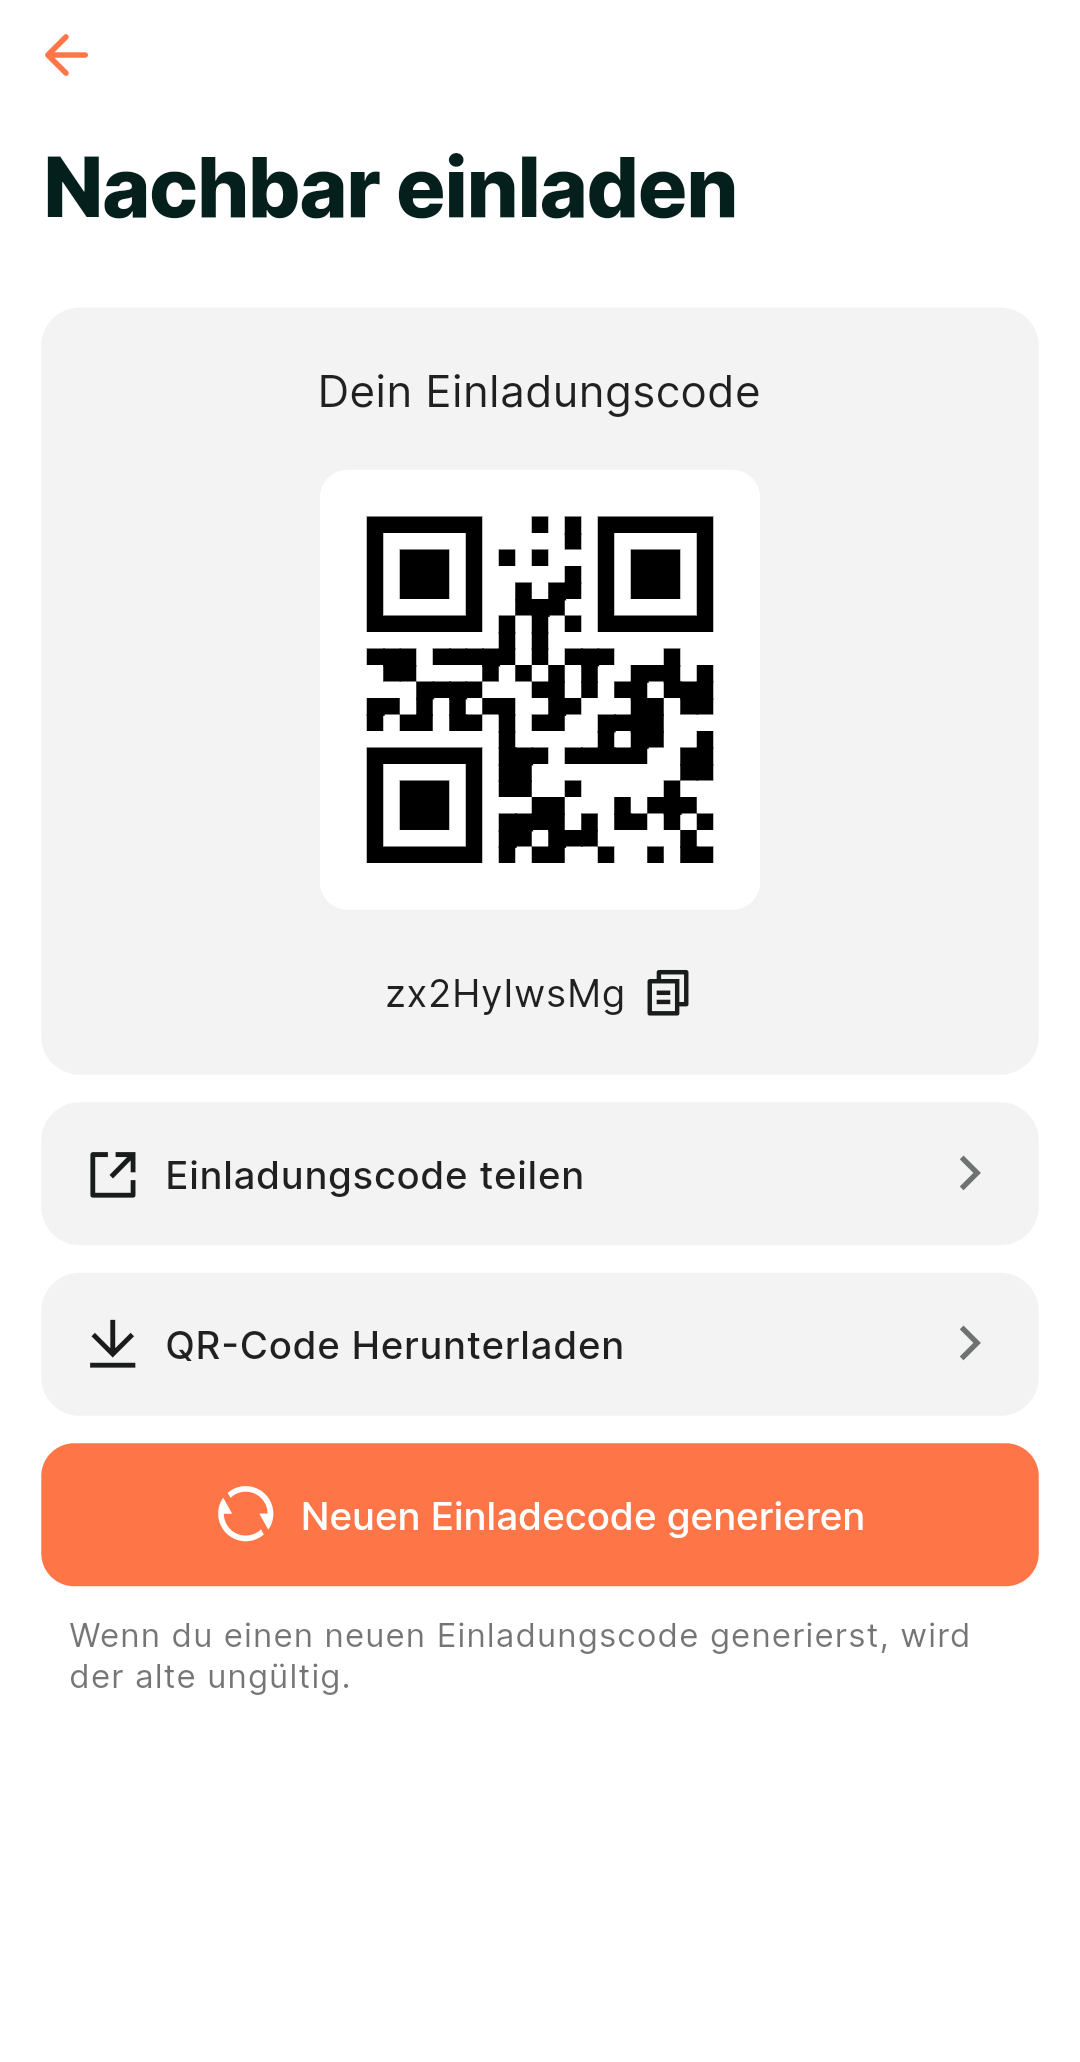
\includegraphics[width=0.3\textwidth]{pics/einladecode-page.png}
  \caption{Smart Replay im Chat}
  \label{fig:einladecode}
\end{figure}

Die Integration des Google Smart Reply ML Kits bietet den Benutzern verschiedene Antwortmöglichkeiten, die direkt über den Eingabefeld des Chats angezeigt werden. Dies ermöglicht eine effizientere und benutzerfreundlichere Kommunikation, da aufwendige manuelle Texteingaben vermieden werden können. Die Abbildung verdeutlicht, wie verschiedene Vorschläge im Eingabefeld angezeigt werden.

Das Google Smart Reply System nutzt die letzten zehn Nachrichten als Kontext, um adäquate und relevante Antwortvorschläge zu generieren. Die Anwendung von maschinellem Lernen in diesem Kontext trägt zur Verbesserung der Benutzererfahrung bei und ermöglicht eine effizientere Kommunikation. Auf diese Weise können die Benutzer schnell und einfach auf eingehende Nachrichten reagieren, wodurch wertvolle Zeit gespart und mögliche Frustrationen vermieden werden.

\subsubsection{Flyer Package}

\subsection{Profil}
\setauthor{Sandin Habibovic}
Die Profilanzeige ist die öffentliche Informationsstelle über den User. In dieser Anzeige werden als erster Eindruck der Name und das Profilbild vom User angezeigt. Genauere Informationen über den User können im Bereich Nutzerinfo gefunden werden. Darunter zählen:
\begin{compactitem}
  \item Geburtstag
  \item Seit wann in der Nachbarschaft
  \item Beruf
  \item Bio
  \item Interessen
  \item Bietet an
\end{compactitem}
Außerdem beinhaltet die Anzeige eine eigene Beitragssicht, wo alle Beiträge vom jeweiligen User eingesehen werden können.
\\
Die folgende Abbildung \ref{fig:public-profile} zeigt, wie das öffentliche Profil in der App dargestellt wird.

\begin{figure}[H]
  \centering
  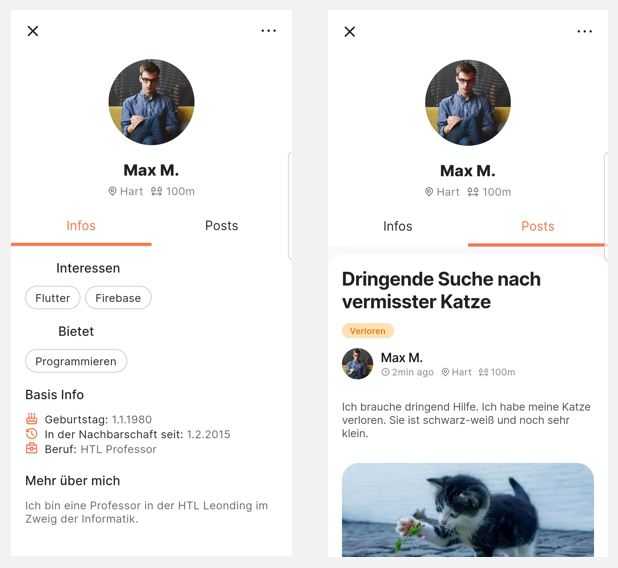
\includegraphics[width=0.6\textwidth]{pics/public-profile.JPG}
  \caption{Öffentliche Profilansicht auf der App}
  \label{fig:public-profile}
\end{figure}

\subsubsection{Profil Melden}
\setauthor{Sandin Habibovic}
Falls das Profil vom User unangebrachten Inhalt aufweist, besteht die Möglichkeit das Profil zu melden.

\subsection{Benachrichtigungen}
\setauthor{Sandin Habibovic}
Benachrichtigungen dienen dazu die Nachbarn über mögliche
Hilfsbereitstellungen zu informieren, bevor der Kontakt
überhaupt entsteht. Die Benachrichtigung zeigt den Nachbarn
an, der in Kontakt treten möchte, und möglicherweise den
Beitrag auf dem geantwortet wurde. Außerdem ist die
Benachrichtigung mit einem „Annehmen“- und „Ablehnen“-
Button ausgestattet, womit das Hilfsangebot angenommen oder
abgelehnt werden kann.

\subsection{Einladecode}
\setauthor{Martin Hausleitner}

\begin{figure}[H]
  \centering
  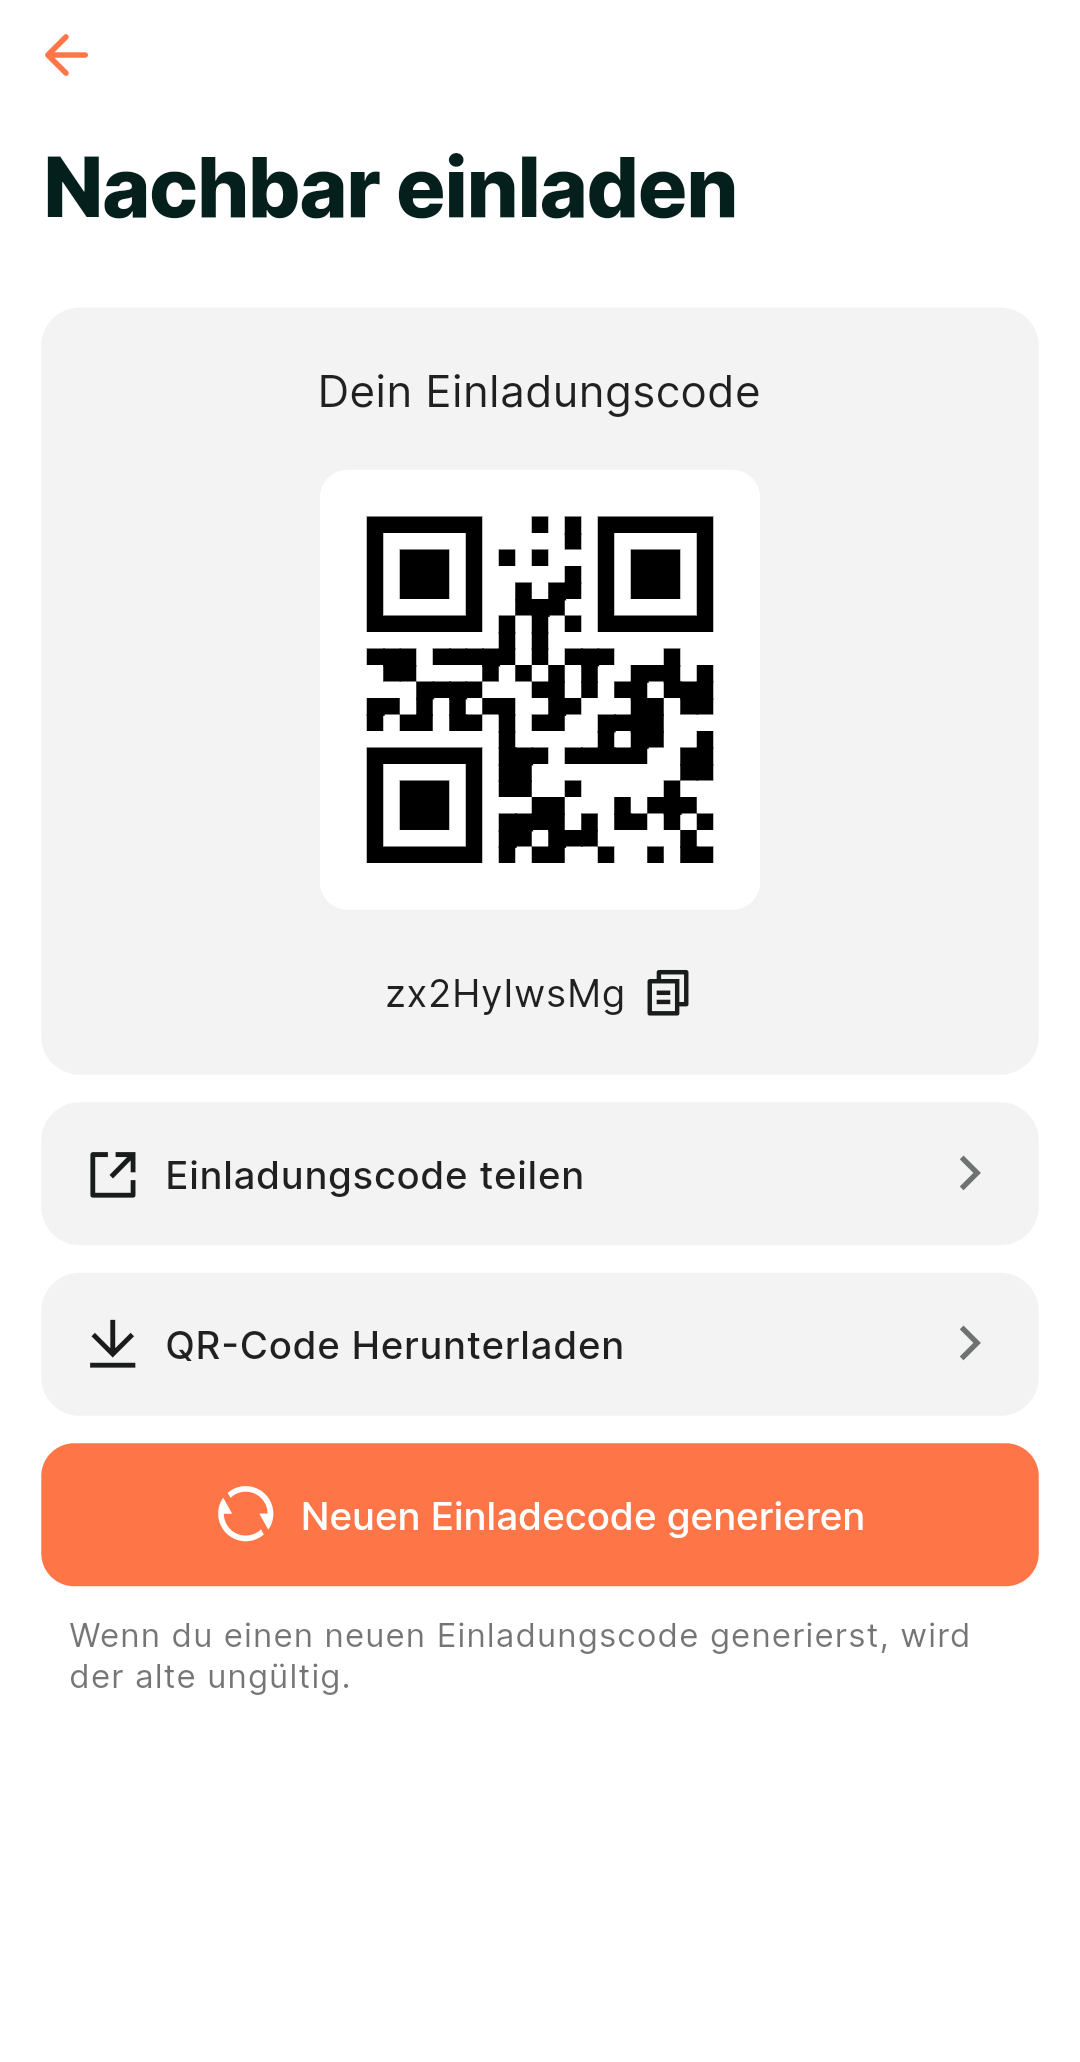
\includegraphics[width=0.3\textwidth]{pics/einladecode-page.png}
  \caption{Einladecode-Seite in der App}
  \label{fig:einladecode}
\end{figure}
Eine der beiden Verifizierungsmethoden basiert auf der Nutzung von Einladungscodes. Als Inspiration diente die deutsche App 'Nebenan', die ebenfalls eine Verifizierung über einen Code ermöglicht. Da das Team dies als gute Lösung erachtete, wurde ein ähnlicher Ansatz übernommen.

Jeder Code hat eine Reichweite von 1 km, ausgehend von der Adresse des Benutzers, der den Code generiert. Dies soll verhindern, dass ein Code missbräuchlich verwendet wird. Der Aktionsradius, in dem der Benutzer den Code nutzen kann, kann von den Administratoren variabel eingestellt werden.

Zudem wird für die Entwickler protokolliert, wer welchen
Code zur Verifizierung verwendet hat, um im Falle eines
Missbrauchs entsprechende Maßnahmen ergreifen zu können, wie
beispielsweise das Sperren des Codes. Administratoren haben
ebenfalls die Möglichkeit, Codes zu deaktivieren.
\subsubsection{Einladungsmöglichkeiten}
\setauthor{Martin Hausleitner}


Folgende Punkte sinder in der Abbildung
\ref{fig:einladecode} zu erkennen.


\begin{enumerate}[label=\arabic*.]
  \item \textbf{Generierung eines QR-Codes:}
        \begin{itemize}
          \item Beim Öffnen der Seite 'Nachbar einladen' wird automatisch ein QR-Code generiert.
          \item Nutzer können den generierten Code in die Zwischenablage kopieren, indem sie den Button neben dem Code betätigen.
        \end{itemize}

  \item \textbf{Teilen des Einladungscodes:}
        \begin{itemize}
          \item Bei dem Button 'Einladungscode teilen' wird eine Nachricht mit dem generierten Code erstellt.
          \item Der Nutzer kann die Nachricht mithilfe des systemspezifischen Sharesheets teilen.
        \end{itemize}

  \item \textbf{Herunterladen des QR-Codes:}
        \begin{itemize}
          \item Unter 'QR-Code herunterladen' wird eine PNG-Datei des Einladungs-QR-Codes erstellt.
          \item Die Datei wird im systemspezifischen Sharesheet geöffnet, um sie speichern zu können.
        \end{itemize}

  \item \textbf{Generierung eines neuen Einladungscodes:}
        \begin{itemize}
          \item Der orangefarbene Button 'Neuen Einladungscode generieren' ermöglicht das Erstellen eines neuen Codes.
          \item Sobald der Nutzer einen neuen Code erstellt, wird der vorherige Code deaktiviert.
        \end{itemize}
\end{enumerate}

Verifizierte Nutzer können alle 24 Stunden einen
Einladungscode generieren.

Die Verifizierung erfolgt, indem der Benutzer bei der
Registrierung die Option 'Mit Einladungscode verifizieren'
auswählt. Anschließend hat er die Möglichkeit, den
Einladungscode entweder über den integrierten
QR-Code-Scanner zu scannen oder manuell einzugeben.


Für die
Implementierung des QR-Code-Scanners wurde das Flutter-Paket
\cite{mobile_scanner} mobile\_scanner
verwendet, welches auf Googles MLKit \cite{googlemlkit}
basiert.

MLKit ist eine Machine-Learning-Bibliothek, die im
vorliegenden Fall für das zuverlässige und schnelle Scannen
von QR-Codes eingesetzt wird.
Diese Bibliothek ermöglicht es, komplexe Funktionen wie das Erkennen von QR-Codes effizient und präzise zu implementieren. Der einzige Nachteil dieses Pakets ist der hohe Speicherbedarf von etwa 10 MB. Daher ist in Zukunft geplant, das MLKit nur bei Bedarf herunterzuladen und nach erfolgreicher Verifizierung des Benutzers wieder zu entfernen.

Der gescannte oder eingegebene Code wird anschließend an die Cloud-Funktion \texttt{checkVerificationCode} (siehe Abschnitt \ref{subsec:registrierung-verify}) gesendet und überprüft, ob der Code korrekt ist.



\subsection{Einstellungen}
\setauthor{Sandin Habibovic}
Die Einstellungssicht der Anwendung bietet eine Reihe an nützlichen Funktionen, die dem User mehr Kontrolle über sein Konto geben.
Dazu gehört zu einem die Option, die Sprache der App umzustellen, um dem User zu ermöglichen, die Anwendung in der bevorzugten Sprache zu nutzen. Zum derzeitigen Stand kann die App sich in zwei Sprachen übersetzen lassen: Deutsch und Englisch.
Darüber hinaus können Benutzer auch entscheiden, ob sie Benachrichtigungen erhalten möchten oder nicht, und diese Einstellungen jederzeit ein- oder ausschalten. Diese Einstellungen bieten den Benutzern eine höhere Privatsphäre und Personalisierungsmöglichkeiten, um die Anwendung besser an ihre individuellen Bedürfnisse anzupassen.
Zu den weiteren Einstellungen gehört das Umändern der E-Mail oder des Passworts, um die Sicherheit des Kontos zu gewährleisten und unbefugten Zugriff zu verhindern.
Die letzte Funktion in der Einstellungssicht ist das Löschen des eigenen Kontos, womit alle Daten des Users gelöscht werden. Vor dem endgültigen Löschen des Kontos wird der User allerdings aufgefordert, seine Entscheidung zu bestätigen.

\subsection{Feedback}
\setauthor{Martin Hausleitner}
Während der Testphase besteht das Ziel darin, eine
effiziente Methode zur Sammlung von Feedback zu finden. Für
ein detailliertes Verständnis von Fehlermeldungen ist die
Bereitstellung von Screenshots äußerst hilfreich. Aus diesem
Grund wurden Packages untersucht, die das Erstellen von
Screenshots ermöglichen und zusätzliche Informationen als
Kontext hinzufügen können.
Das ausgewählte Package ist \cite{feedback}.
Dieses erlaubt es den Nutzern, Screenshots anzufertigen, Annotationen hinzuzufügen und anschließend einen entsprechenden Textkontext einzufügen. Eine nützliche Funktion ermöglicht es den Nutzern, bei Bedarf erneut zu navigieren und den Screenshot zu wiederholen.

Um den Feedback-View zu initiieren, wurde das Package
\cite{shake} shake verwendet.
Dieses wird durch eine bestimmte Bewegung des Mobilgeräts aktiviert. Bei der Implementierung dieser Funktion wurden ähnliche Mechanismen berücksichtigt, die in anderen Anwendungen zur Feedback-Erhebung verwendet werden.

Das von uns gewählte Vorgehen zur Analyse des Feedbacks erfolgt über die Trello-API, welche es uns ermöglicht, ein entsprechendes Dashboard zur Erfassung und Bearbeitung der Meldungen zu erstellen. Die erfassten Informationen, wie beispielsweise der Screenshot, der Text, das Datum und relevante Systeminformationen, dienen uns als Grundlage für eine weitere Auswertung und Fehlerbehebung. Trello erleichtert uns die Verwaltung des Feedbacks auf kostenlose Weise und stellt somit ein adäquates Instrument zur Unterstützung des Entwicklungsprozesses dar.


\section{UI/UX Design}
Das Design der Nachbarschafts-App war für das Team von hoher Bedeutung, weshalb der Designer Martin Hausleitner erheblichen Zeit- und Arbeitsaufwand aufwendete, um ein anspruchsvolles Design zu gestalten. Angesichts der Tatsache, dass die App ein breites Publikum ansprechen soll, einschließlich verschiedener Altersgruppen, war es von entscheidender Bedeutung sicherzustellen, dass die Benutzer die App einfach und intuitiv bedienen können. Um dieses Ziel zu erreichen, wurde eine klare Struktur und Navigation in das Design integriert, um den Benutzern eine einfache und effektive Nutzung der gewünschten Funktionen zu ermöglichen. Es wurde darauf geachtet, dass die Buttons gut erkennbar und mit aussagekräftigen Icons und verständlichen Beschriftungen versehen sind, um Verwirrung zu vermeiden. Weiterhin wurde das Design der Karten auf eine organische Weise gestaltet, um ein harmonisches und ästhetisches Gesamtbild zu erzeugen.
\setauthor{Martin Hausleitner}
\subsection{Inspiration}
Während des Designprozesses für die App wurden umfangreiche Recherchen im Bereich App-Design durchgeführt. Das Ziel war, die App so intuitiv wie möglich zu gestalten, um eine benutzerfreundliche Erfahrung sicherzustellen. Dabei wurden bekannte Social-Media-Apps wie Twitter\cite{twitter}, Instagram\cite{instagram} und TikTok\cite{tiktok} als Orientierung genutzt, da diese bereits erfolgreich auf dem Markt etabliert sind und von vielen Menschen vertraut genutzt werden.

Zusätzlich diente die erfolgreichste Nachbarschafts-App in Deutschland, Nebenan\cite{nebenan}, als Grundlage für die App-Entwicklung. Allerdings wurde festgestellt, dass ihre App sehr kompliziert aufgebaut und unübersichtlich ist. Daher wurde dies als Chance gesehen, um es besser zu machen.

Zur Entwicklung eines einfachen und schlichten Designs wurden Inspirationen von Websites wie Dribble\cite{dribble} und Mobbin\cite{mobbin} genutzt. Insgesamt war die Recherche und Inspiration für das Design der App ein wichtiger Schritt, um sicherzustellen, dass Benutzer eine ansprechende und intuitive Erfahrung haben.

\subsection{Prototyping}
Das Team legte von Anfang an großen Wert auf eine exzellente
Benutzererfahrung, und daher war es ihnen klar, dass ein
Prototyp gestaltet werden musste. Das Prototyping hatte für
die Entwickler den großen Vorteil, dass sie beim
Programmieren in Flutter nicht mehr lange darüber nachdenken
mussten, wie Menüs oder Bildschirme gestaltet werden
sollten. Somit war es einfach für Teammitglieder, die nicht
mit Design vertraut waren, den Prototypen als Grundlage zu
nutzen, um ihre Umsetzung in Flutter zu gestalten. Der
Prototyp selbst war für den Designer Martin Hausleitner eine
Reise durch verschiedene Designer-Tools, die im folgenden
Absatz genauer behandelt werden.


\subsubsection{Framer}

Framer ist eine Software, die es Benutzern ermöglicht, schnell und einfach ansprechende Prototypen von mobilen Anwendungen und Websites zu erstellen. Das Tool wurde ursprünglich als Prototyping-Tool für Designer entwickelt, um Designs schnell zu testen und zu verfeinern, bevor sie in die Entwicklung übergehen.

Erfolgreiche Apps wie Spotify haben Framer im Rahmen ihres
Prototyping-Prozesses verwendet, um schnell und effizient
funktionierende App-Designs zu erstellen. Framer ist eine
schnelle und effiziente Möglichkeit, um Ideen in die Tat
umzusetzen, ohne sich durch langwierige Entwicklungsprozesse
zu quälen. Dies sind überzeugende Gründe für den Designer, den ersten Prototypen mit Framer zu gestalten.

\begin{figure}[h]
  \centering
  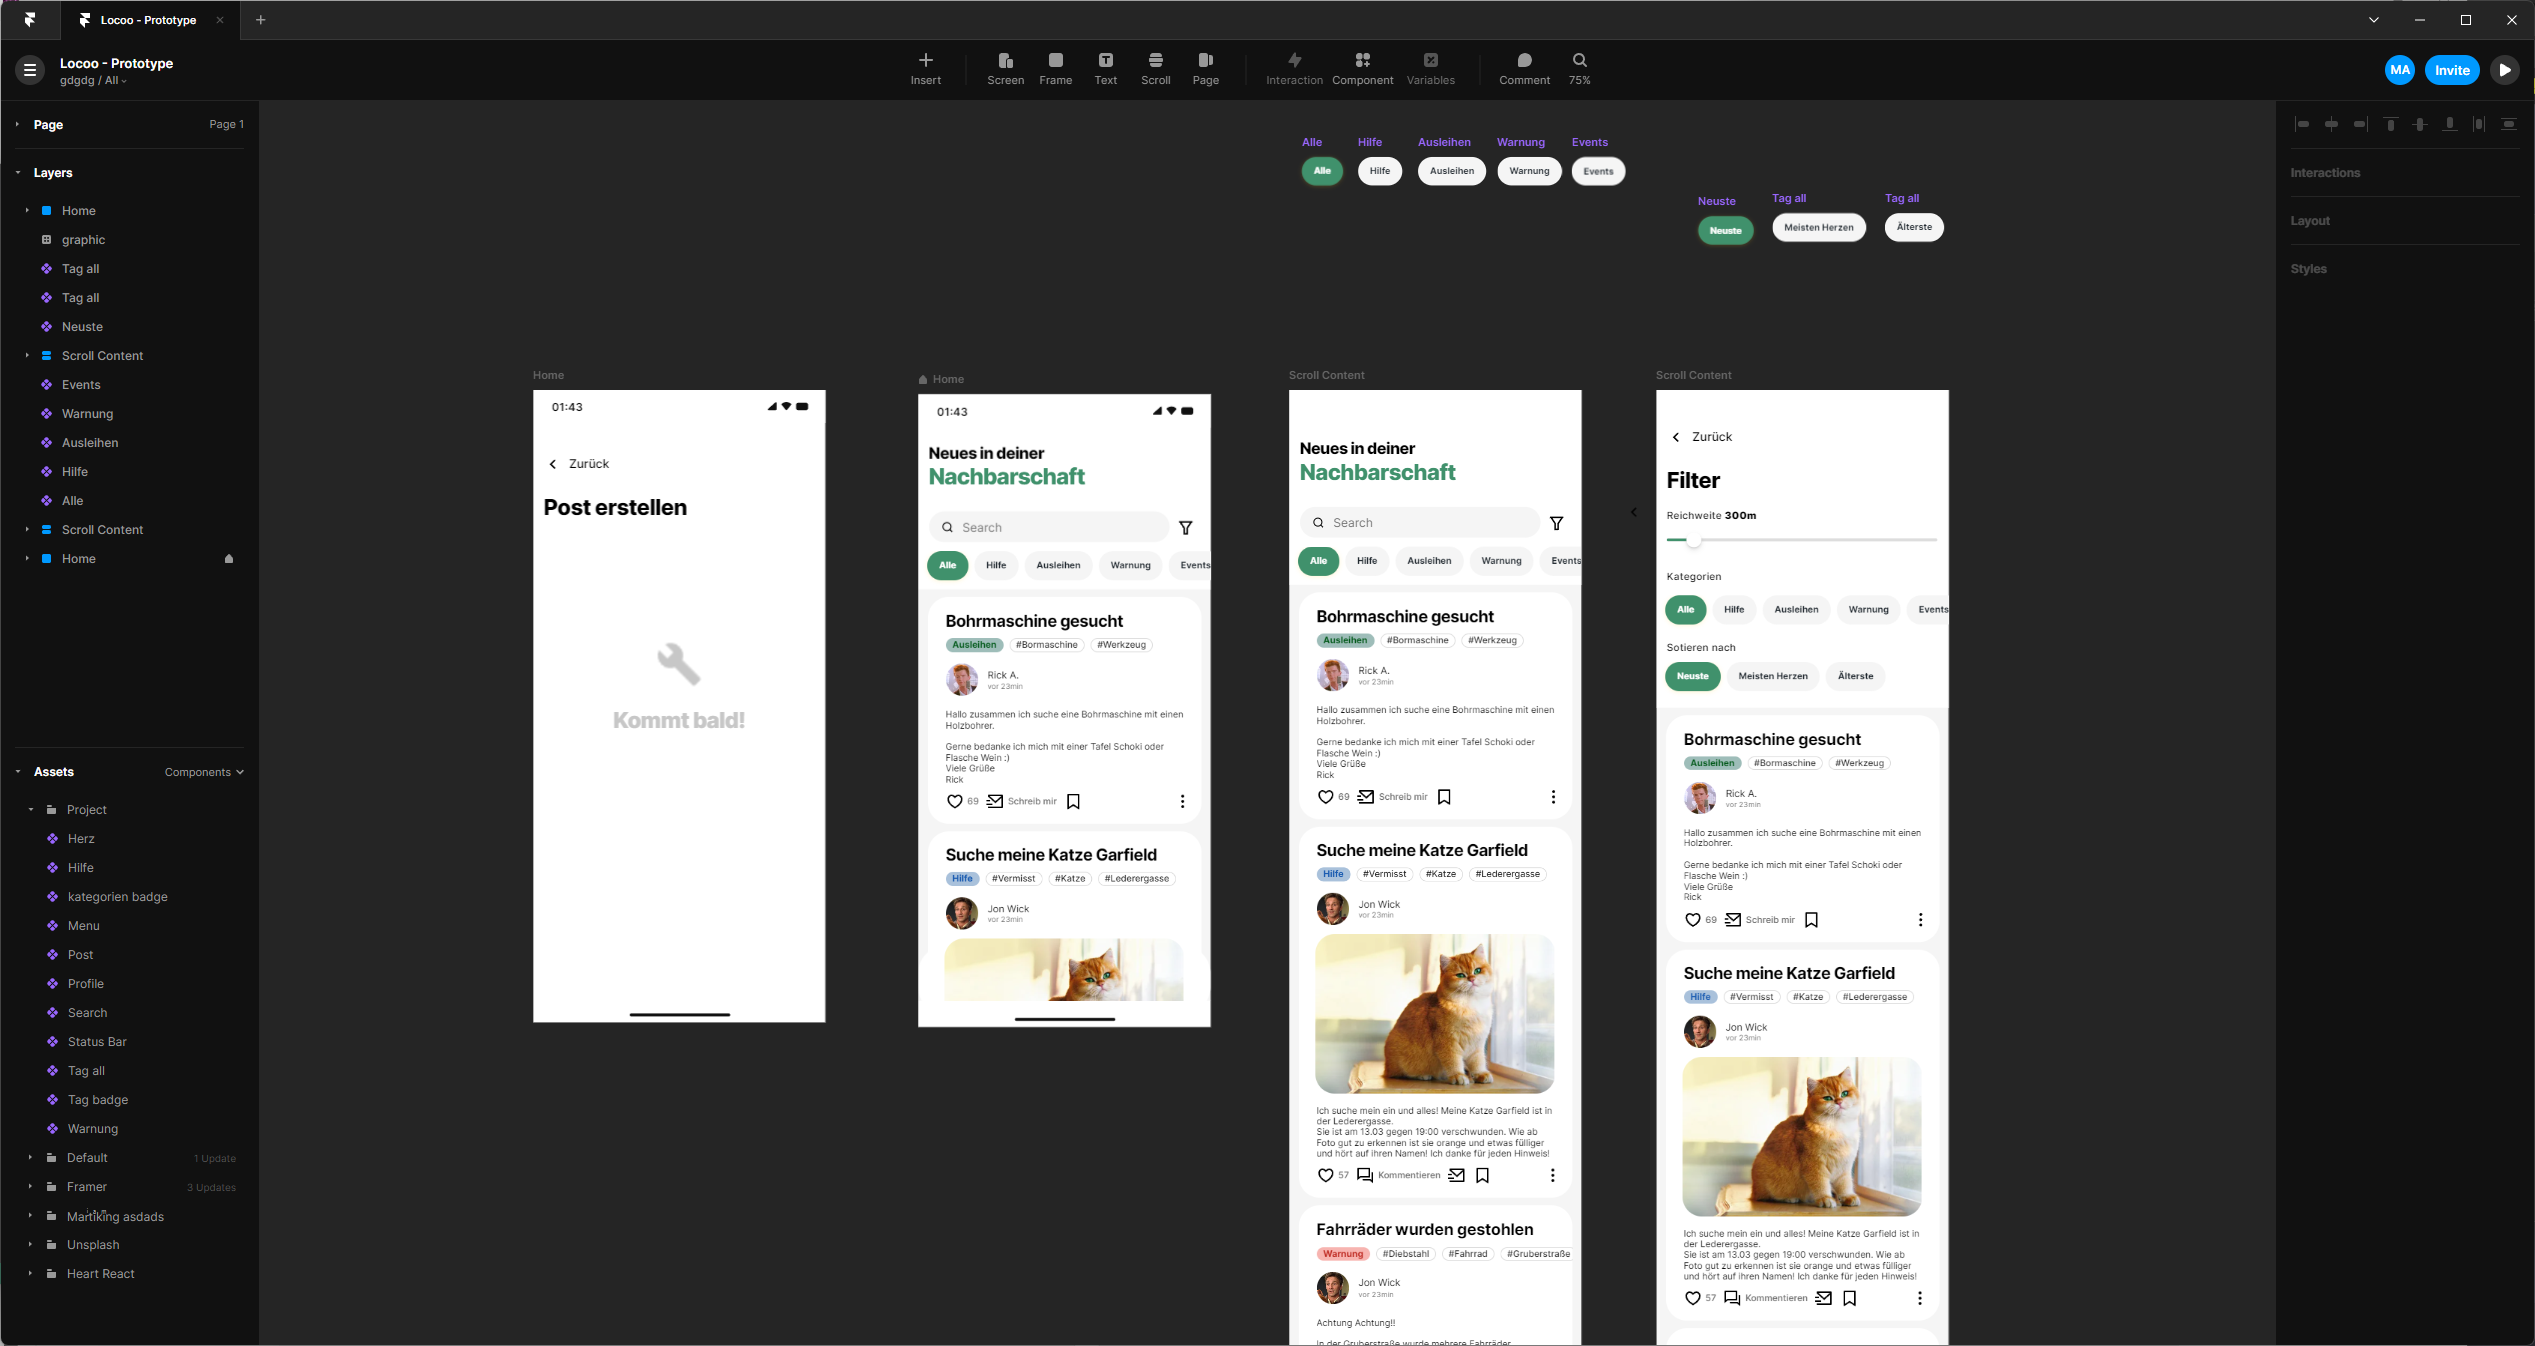
\includegraphics[width=1\textwidth]{pics/nochba-framer-prototype-screenshot.png}
  \caption{Nochba Prototyp in Framer}
  \label{fig:framer-prototype}
\end{figure}


Framer wurde während des Hackerthon Linz haCKt verwendet, um
den ersten Prototypen zu erstellen wie bei der man bei der
Abbildung \ref{fig:framer-prototype} erkennen kann. Die Wahl von Framer war
aufgrund seiner Geschwindigkeit und Effizienz in der
Erstellung von funktionsfähigen App-Designs und der
Erfahrung, die der Benutzer bereits mit dem Tool hatte,
getroffen worden.

Seit der Erstellung des ersten Prototyps hat sich das Geschäftsmodell von Framer jedoch geändert. Es ist jetzt ein Website-Baukasten, der es Benutzern ermöglicht, einfach und schnell ansprechende Websites zu erstellen, ohne Kenntnisse in der Webentwicklung zu benötigen. Obwohl es nun als Website-Baukasten fungiert, behält Framer immer noch einige seiner Kernfunktionen als Prototyping-Tool bei, was es zu einer guten Option für Designer und Entwickler macht, die schnell Prototypen erstellen möchten.

Insgesamt hat Framer gezeigt, dass es ein schnelles und effektives Tool ist, um Designideen in die Tat umzusetzen. Obwohl es nun als Website-Baukasten fungiert, ist es immer noch eine nützliche Option für Designer und Entwickler, die schnell und einfach Prototypen erstellen möchten.

\subsubsection{Adobe XD}
Bei der ersten Nutzung von Framer wurden zahlreiche Funktionen und Optionen entdeckt, was zunächst begeisterte. Doch mit der Zeit wurde erkannt, dass dies für das betreffende Projekt zu umfangreich war und somit nach einer einfacheren Lösung gesucht werden musste. Die Wahl fiel auf Adobe XD, da bereits jahrelange Erfahrung mit diesem Tool vorhanden war.

Trotz des geringeren Funktionsumfangs im Vergleich zu Framer
ist Adobe XD aufgrund seiner Benutzerfreundlichkeit und
Einfachheit ein ideales Werkzeug, um schnell Prototypen zu
erstellen. Alle Hauptscreens wurden fertiggestellt wie man
bei Abbildung \ref{fig:adobexd-prototyp} sehen kann, bevor
die Entwicklung mit Flutter begann. Die anderen wichtigen
Screens wurden später gestaltet, nachdem eine bessere
Kenntnis von Flutter erlangt wurde und es möglich war, den
Aufwand für die Umsetzung besser abzuschätzen.

\begin{figure}[h]
  \centering
  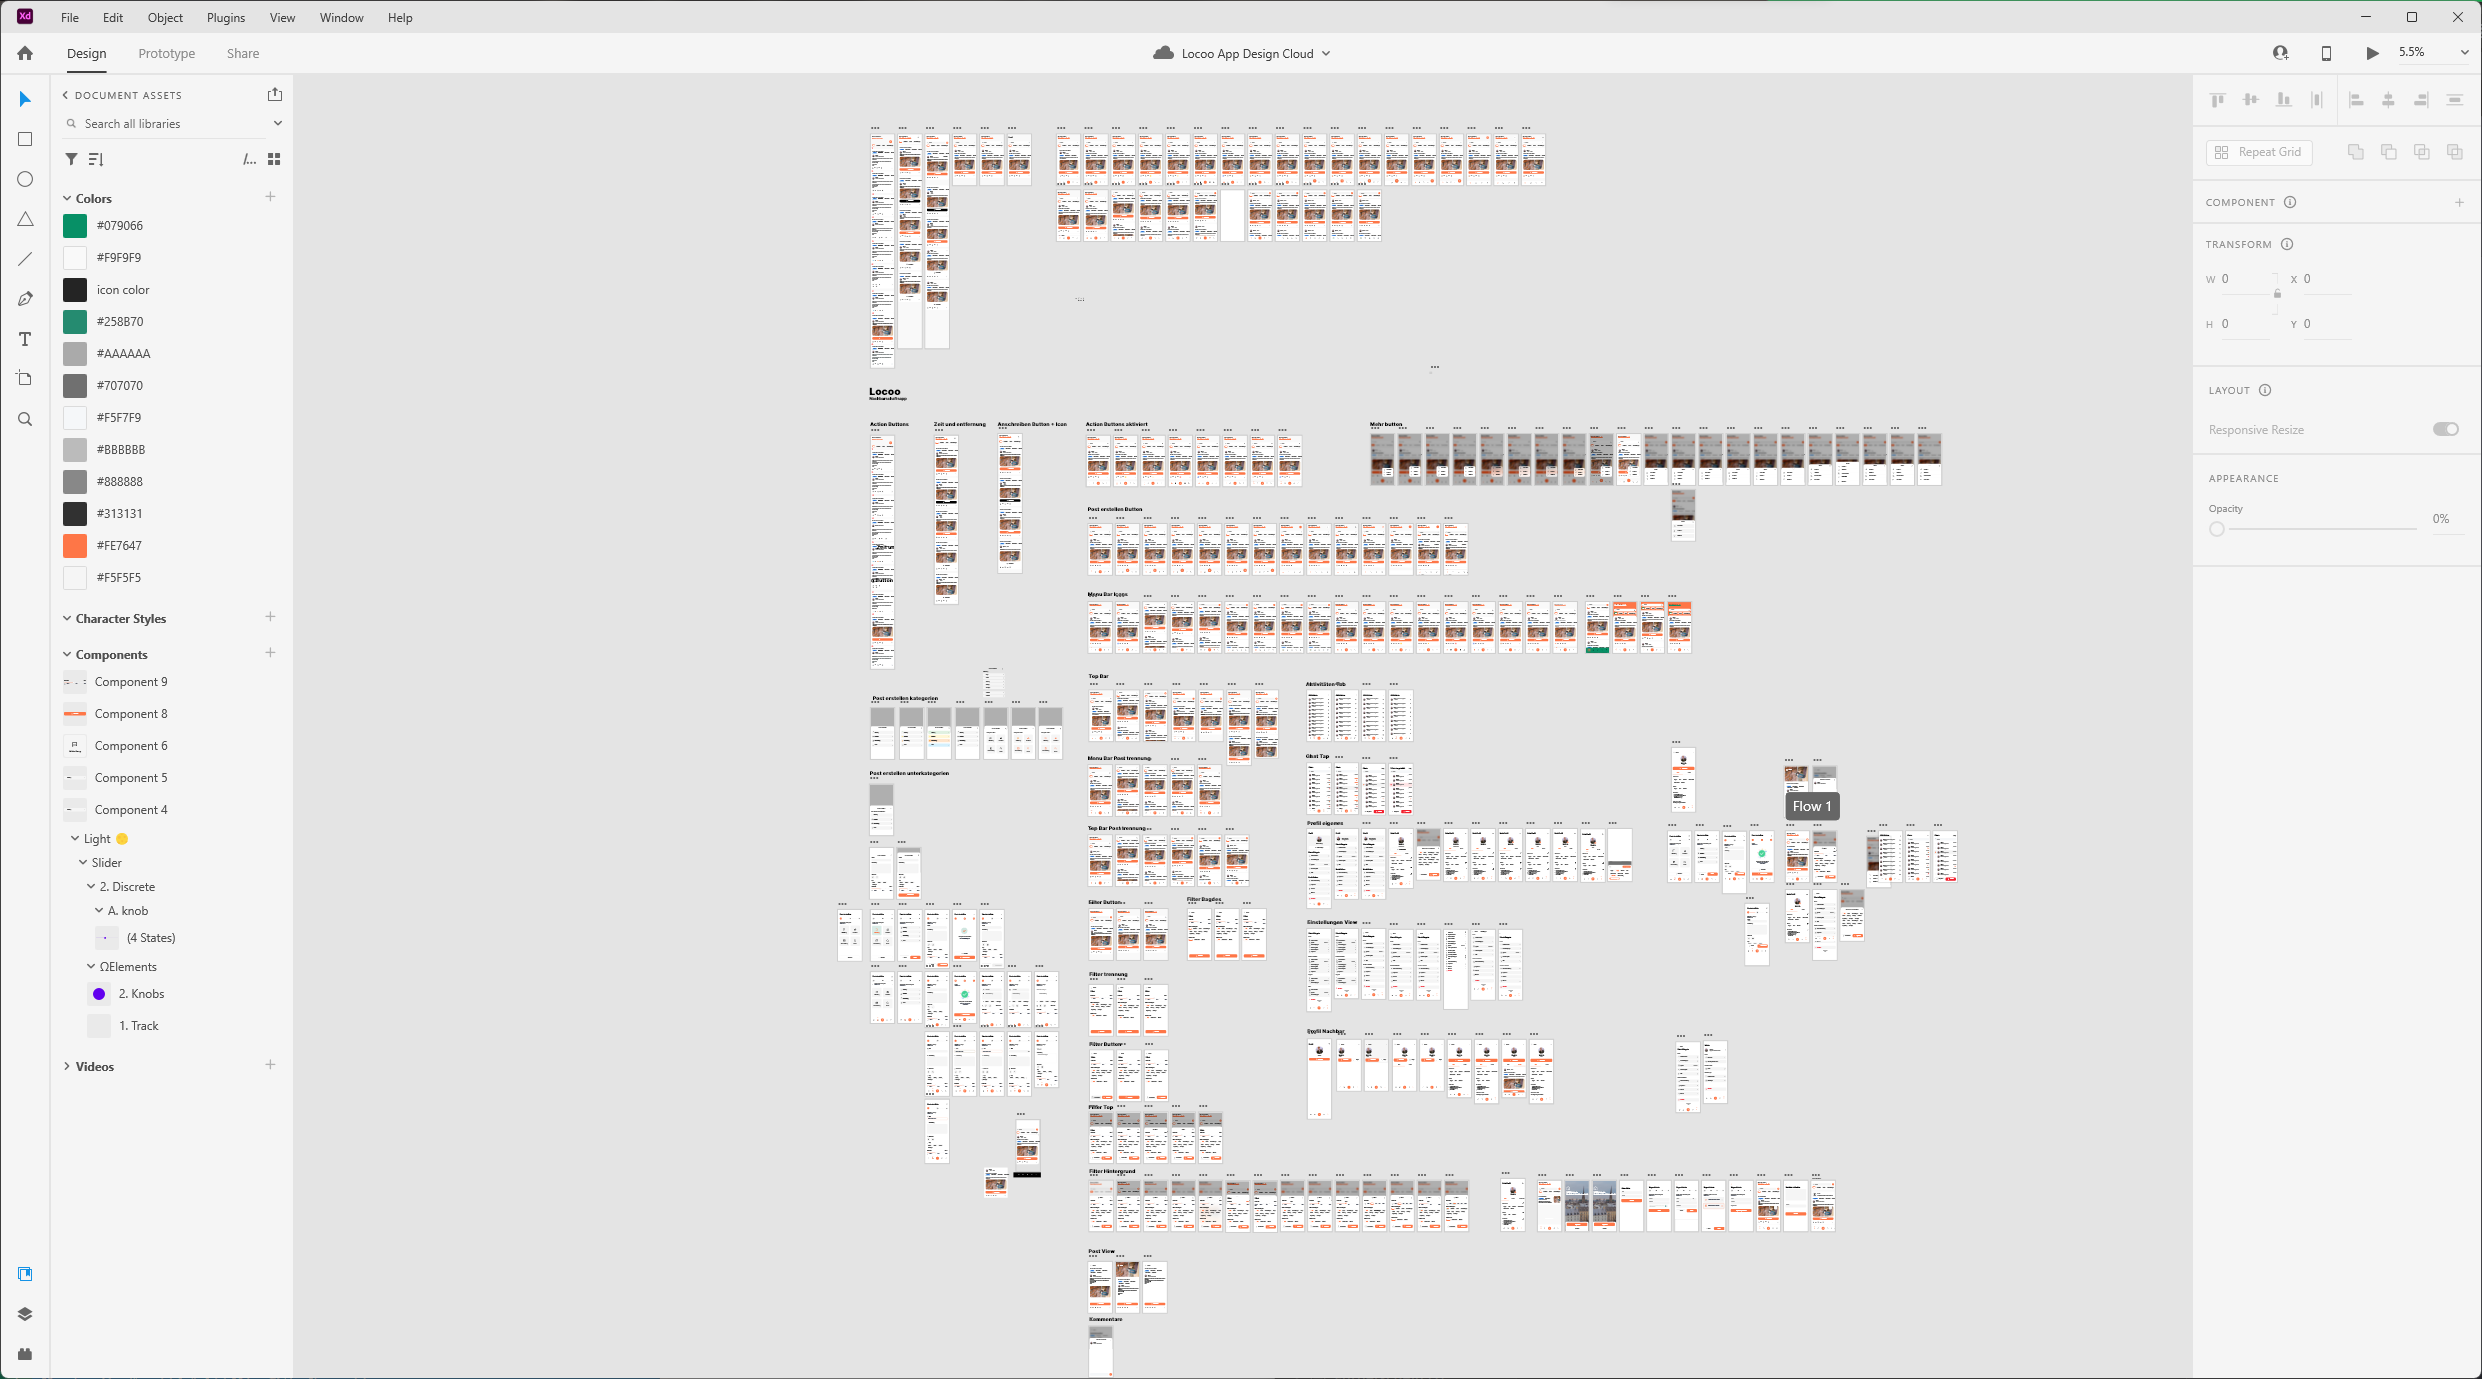
\includegraphics[width=0.95\textwidth]{pics/nochba-adobe-xd-protoype-screenshot.png}
  \caption{Nochba Prototyp in Adobe XD}
  \label{fig:adobexd-prototyp}
\end{figure}

Die Abbildung \ref{fig:adobexd-prototyp} zeigt eine Sammlung von Designs und Designentwicklungen im Prototypen. Adobe XD erwies sich als passend für das Projekt, da Martin Hausleitner, der alleinige Designer, keine Kollaborationsfunktionen benötigte. Das Tool ermöglichte es ihm, verschiedene Designvarianten effizient zu entwickeln und zu optimieren, um eine ansprechende Benutzeroberfläche für die Anwendung zu erstellen.

Jedoch ist der Designer mit
dem bekannteren und kostengünstigeren Figma vertraut, das
bei der Zusammenarbeit an einem Design und aufgrund der
zusätzlichen Funktionen besser geeignet ist.

Zusammenfassend kann festgestellt werden, dass Adobe XD ein leistungsstarkes Tool für UI/UX-Designer ist, das einfach zu bedienen ist und für kleine bis mittelgroße Projekte geeignet ist. Obwohl es nicht so viele Funktionen wie andere Tools bietet, eignet es sich gut für die schnelle Erstellung von Prototypen und eine einfache Zusammenarbeit mit Entwicklern und Stakeholdern.

\subsubsection{Design System}
\begin{figure}[h]
  \centering
  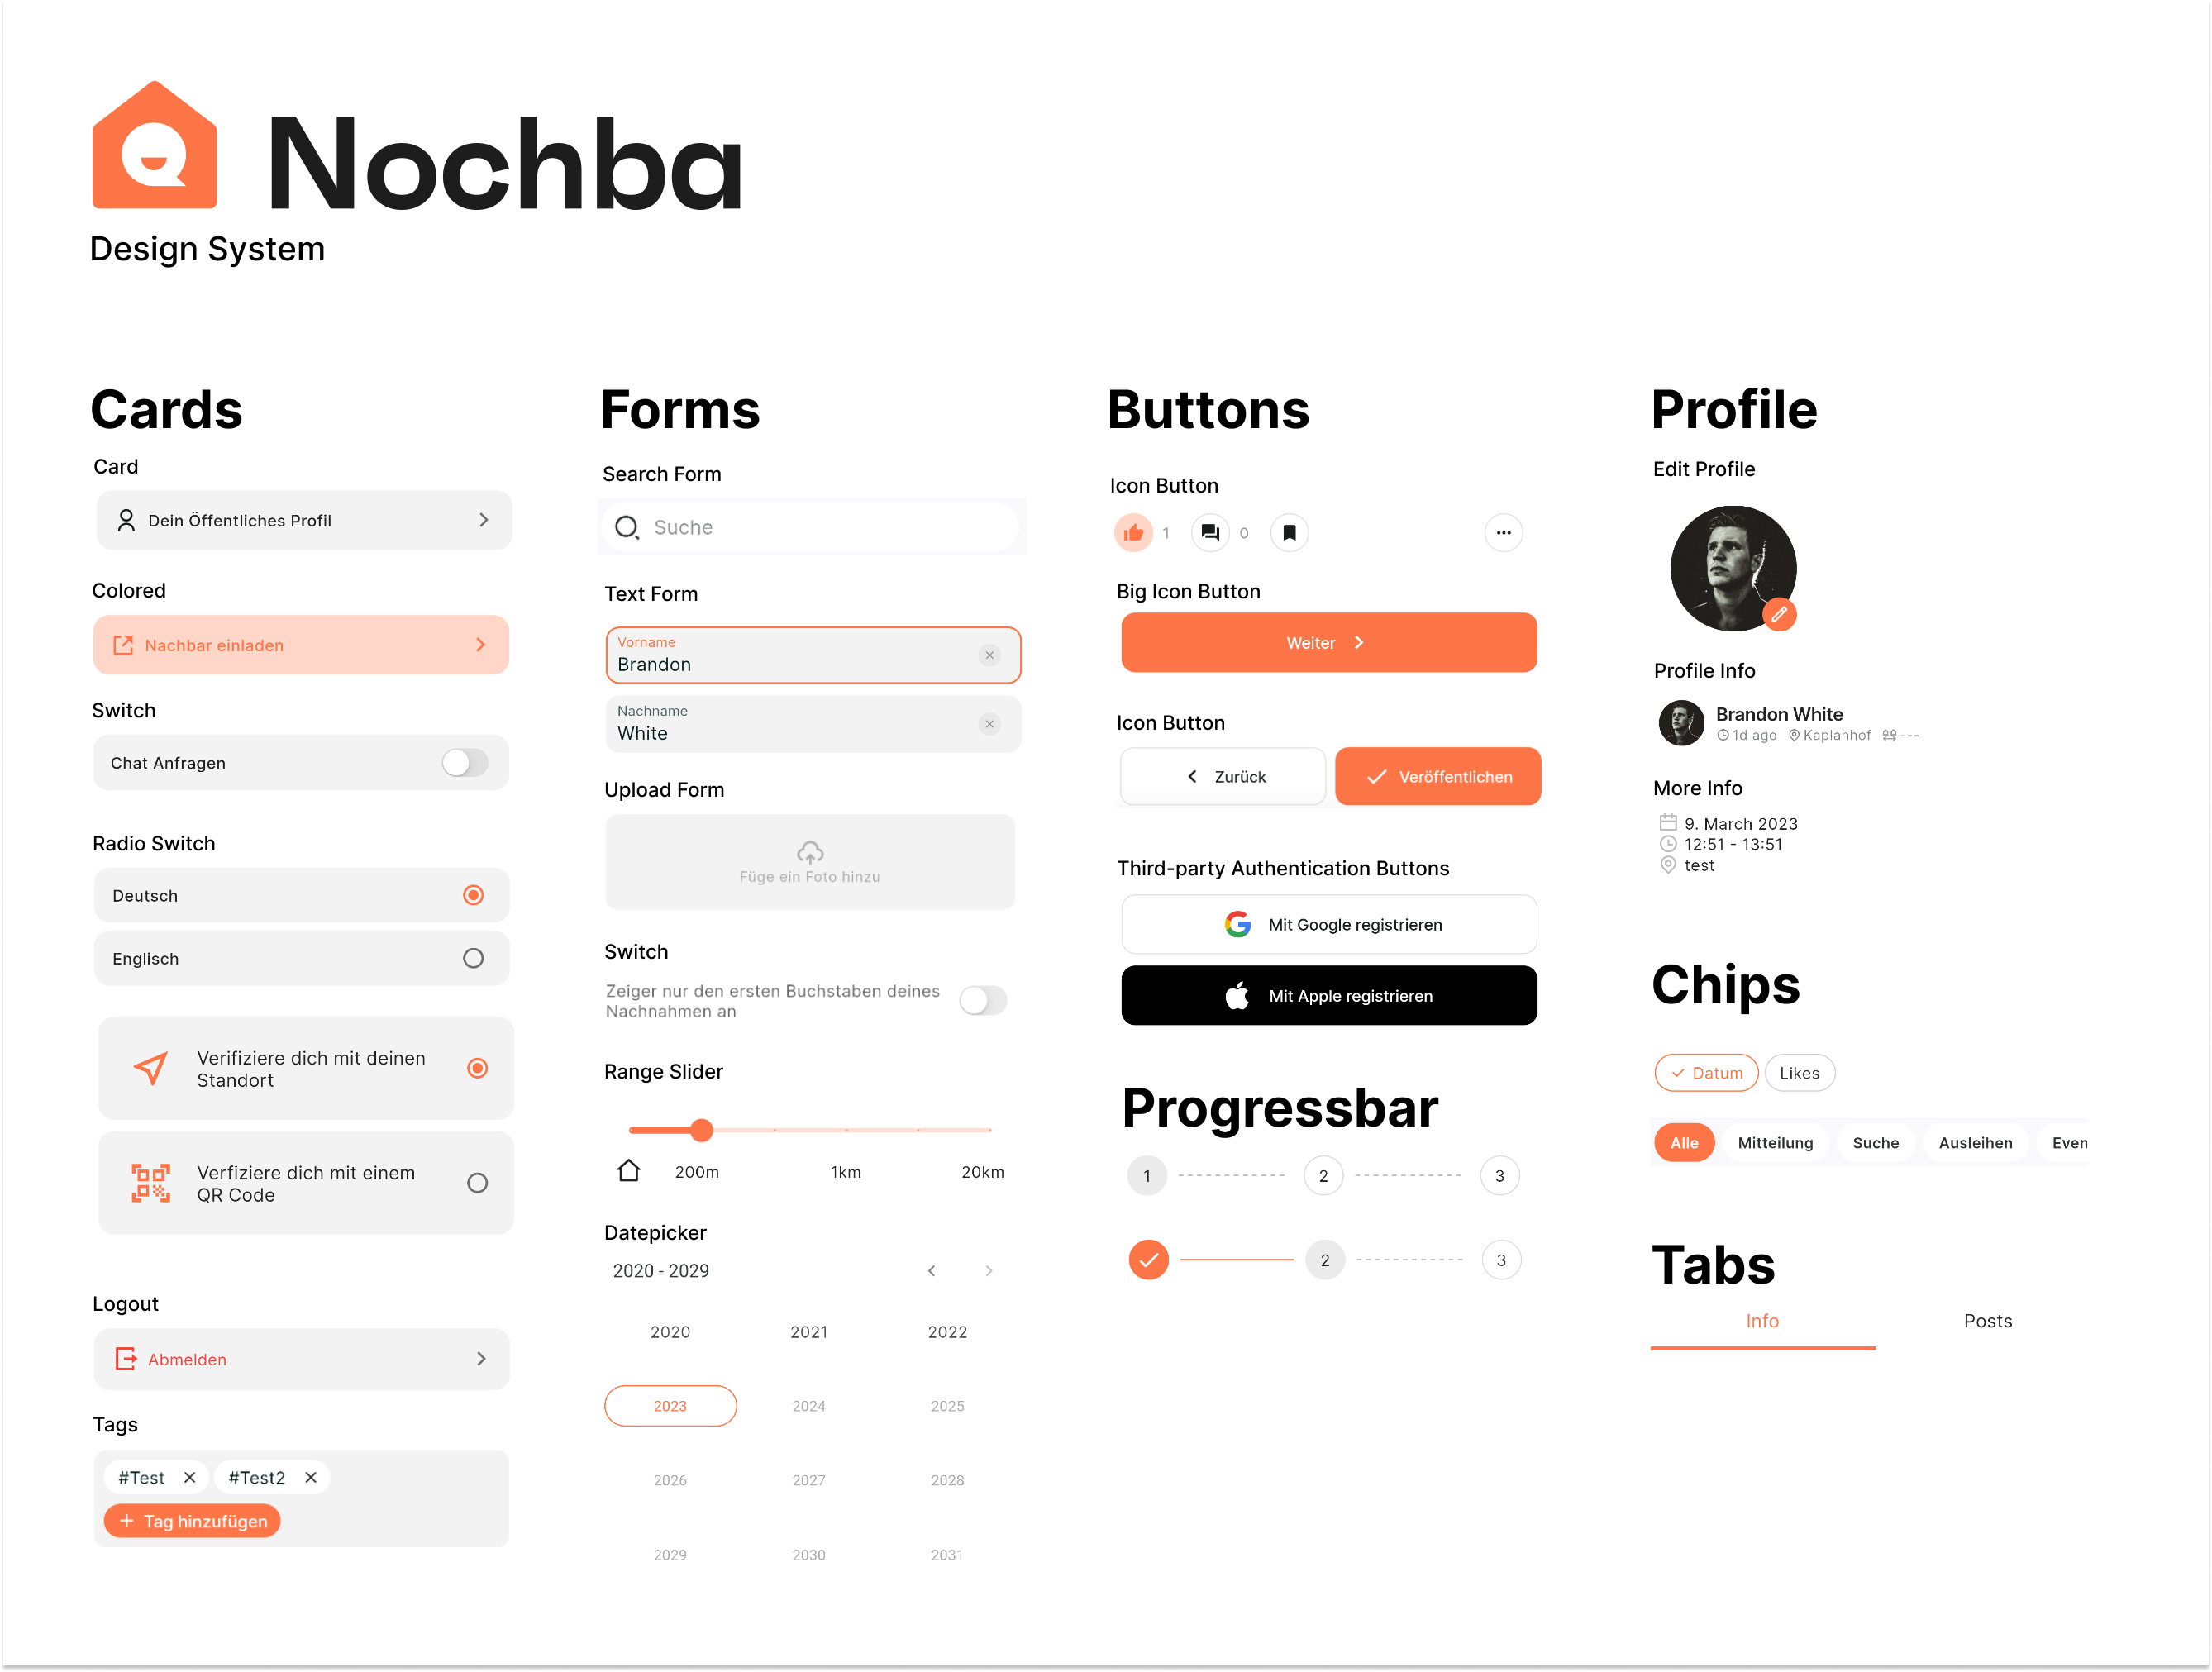
\includegraphics[width=1\textwidth]{pics/design-system.png}
  \caption{Nochba Design System}
  \label{fig:design-system}
\end{figure}

Der Designer Martin Hausleitner hat ein Design-System
entwickelt, um bei der Gestaltung der App eine klare
Struktur zu haben. Das System umfasst verschiedene
UI-Elemente, von denen die wichtigsten in Abbildung
\ref{fig:design-system} dargestellt sind.

\paragraph{Cards}\mbox{} \\

Ein häufig genutztes UI-Element in der App ist das Card-Design. Der Designer hat hierbei darauf geachtet, alle Elemente in einem abgerundeten, grauen Container mit hellem Grau zu gestalten, um einen guten Kontrast zum Hintergrund zu erzeugen.

Um den Nutzer zur Interaktion aufzufordern, wurde beispielsweise eine Einladungskarte für Nachbarn gestaltet, die in den Primär- und Sekundärfarben gehalten ist.

Für die Switch Card wurde das Switch-Design des verfügbaren Cupertino UI-Widgets genutzt, da es dem Designer gut gefiel.

Für den Radio Switch gibt es eine größere und eine kleinere Variante, um verschiedenen Design-Anforderungen gerecht zu werden.

Der Logout-Button wurde bewusst mit einem roten Icon und roter Schrift gestaltet, um dem Nutzer deutlich zu machen, dass er sich ausloggt.

Besondere Aufmerksamkeit erforderte der Tag-Editor, der einer der aufwändigsten Widgets in Flutter war. Der Designer hat diesen komplett neu durchdacht, um das Erstellen und Abspeichern von Tags leicht verständlich zu gestalten, so dass jeder Nutzer damit umgehen kann.

\paragraph{Forms}\mbox{} \\
Das Suchformular wurde mit einem organisch runden Design gestaltet, das zum Feed-Screen der App passt. Die Formulare, die in der gesamten App verwendet werden, wurden in Flutter sehr aufwändig gestaltet, um den Vorgaben des Designers zu entsprechen.

Um dem Nutzer eine klare Rückmeldung zu geben, wurde ein
orangefarbener Ring um das angeklickte Feld platziert. Es
wurde darauf geachtet, dass das Label des Textfeldes immer
gut lesbar ist auch wenn Cursor innerhalb des Feldes
ist. Zudem wurde ein X-Button hinzugefügt, der den gesamten
Inhalt des Textfelds löscht.

Darunter befindet sich ein Upload-Formular, das im Design einer großen Card gestaltet ist, um dem Nutzer das Klicken zu erleichtern.

Der Switch, der in den Formularen verwendet wird, wurde aus dem iOS-Design übernommen.

Der Range-Slider wurde unter Verwendung des Material Designs gestaltet und mit den passenden Farben angepasst. Zusätzlich wurden Labels hinzugefügt, um dem Nutzer eine bessere Orientierung zu ermöglichen.

Für den Datepicker wurde die Bibliothek
Syncfusion flutter datepicker

\cite{syncfusion_flutter_datepicker} verwendet. Das UI wurde
entsprechend den Farben der App angepasst, um eine
konsistente und ästhetische Benutzeroberfläche zu
gewährleisten.

\paragraph{Buttons}\mbox{} \\
Die Icon-Buttons stellten das aufwändigste Design-Element
dar, da es bei Flutter mehrere Möglichkeiten gibt, um sie zu
implementieren. Dies führte dazu, dass sie häufig geändert
werden mussten, um das richtige Design zu finden. Die
runden Icon-Buttons ziehen sich durch die gesamte App.

Der Big Icon Button wurde häufig eingesetzt, da er die Primary Color aufweist und somit eine wichtige Funktion anzeigt. Dem Designer war es wichtig, dass jeder Button immer ein Icon hatte, um dem Nutzer die Bedienung zu erleichtern. Es wurde darauf geachtet, dass alle Buttons die gleiche Rundung aufweisen.

Für den normalen Icon-Button wurde ein dezenter grauer Hintergrund verwendet, um ihn als Secondary Button zu kennzeichnen. Auch hier wurden immer Icons verwendet.

In der App wurden zusätzlich Third-Party-Anmeldemöglichkeiten Buttons integriert. Dazu gehören das Login mit Apple und das Login mit Google. Um eine konsistente Benutzeroberfläche sicherzustellen, wurden diese Anmeldeoptionen entsprechend an das Design angepasst.

Die Progressbar wurde beim Registrierungsprozess und beim
Erstellen eines Posts eingesetzt, um dem Nutzer eine bessere
Orientierung zu geben, wie viele Schritte noch zu erledigen
sind. Ursprünglich war geplant, das Design von Material zu
nutzen. Aufgrund der Einschränkungen bei der Umsetzung des
Designs mit dem Material-Design in Flutter und den spezifischen
Anforderungen des Designers, war es erforderlich, die
Progressbar komplett in Flutter zu gestalten.

\paragraph{Profile}\mbox{} \\
Der Edit Profile-Button wurde beim Registrieren und
Bearbeiten eines Profils verwendet, um das Profilbild
zu ändern. Es wurde darauf geachtet, dass der Button
auffällig ist, damit der Nutzer ihn schnell erkennen kann.

Die Profil-Informationen werden bei jedem Beitrag angezeigt,
darunter die Zeit, in welchem Stadtteil der Nachbar wohnt
und die ungefähre Entfernung zu ihm. Es wurde darauf
geachtet, dass die Informationen übersichtlich mit
Icons dargestellt werden, um dem Nutzer eine schnelle Orientierung
zu ermöglichen.

More Info wird beispielsweise bei einem Event-Eintrag oder
den persönlichen Daten eines Profils verwendet. Hier wurden
Icons verwendet, um dem Nutzer eine einfache und
verständliche Darstellung zu ermöglichen.

\paragraph{Chips}\mbox{} \\
Chips kommen in der App häufig zum Einsatz, um Filter auszuwählen. Der Designer ist allerdings mit dem finalen Design noch nicht vollständig zufrieden, da es zahlreiche unterschiedliche Varianten gibt. Die Gestaltung der Chips wird weiterhin optimiert, um eine einheitliche und ästhetisch ansprechende Darstellung zu erreichen. Dieser fortlaufende Prozess zeigt das Bestreben, die Benutzeroberfläche kontinuierlich zu verbessern und den Anforderungen der Benutzer gerecht zu werden.

\paragraph{Tabs}\mbox{} \\
Die Implementierung von Tabs war auch in Flutter eine
Herausforderung, da die Positionierung nicht der
Standard-Tabs-Position entsprach. Aus diesem Grund wurde die
Gestaltung aufwändig gestaltet, um ein optimales Ergebnis zu
erzielen. Die Mühe hat sich jedoch gelohnt, da die Tabs nun
eine gute funktionale Benutzeroberfläche bieten.

\subsubsection{Farben}S
Die Farbpalette einer Marke spielt eine wichtige Rolle im UI-Design, da sie dazu beiträgt, ein konsistentes Erscheinungsbild zu schaffen. Bei der Gestaltung einer Nachbarschafts-App wurde eine Vielzahl von Farbpaletten von anderen Apps untersucht. Es wurde festgestellt, dass die meisten großen Apps die Farbe Grün verwenden.

Obwohl Grün oft mit Natur und Gemeinschaft assoziiert wird, wurde sich bewusst dazu entschieden, sich von diesen etablierten Konventionen abzuheben. Stattdessen wurde die Farbe Orange ausgewählt, da sie auffällig und ungewöhnlich ist und somit das Potenzial hat, die App von anderen Nachbarschafts-Apps zu unterscheiden.

Zusätzlich passt die Farbe Orange gut zu den Werten der App, da sie für Wärme, Freundschaft und Optimismus steht - Eigenschaften, die in der App gefördert werden sollen. Die Hoffnung besteht darin, dass die Farbauswahl dazu beitragen wird, dass die Nutzer sich in der App wohl und willkommen fühlen und die Farbe sich als wiedererkennbares Markenzeichen etabliert.


\begin{figure}[h]
  \centering
  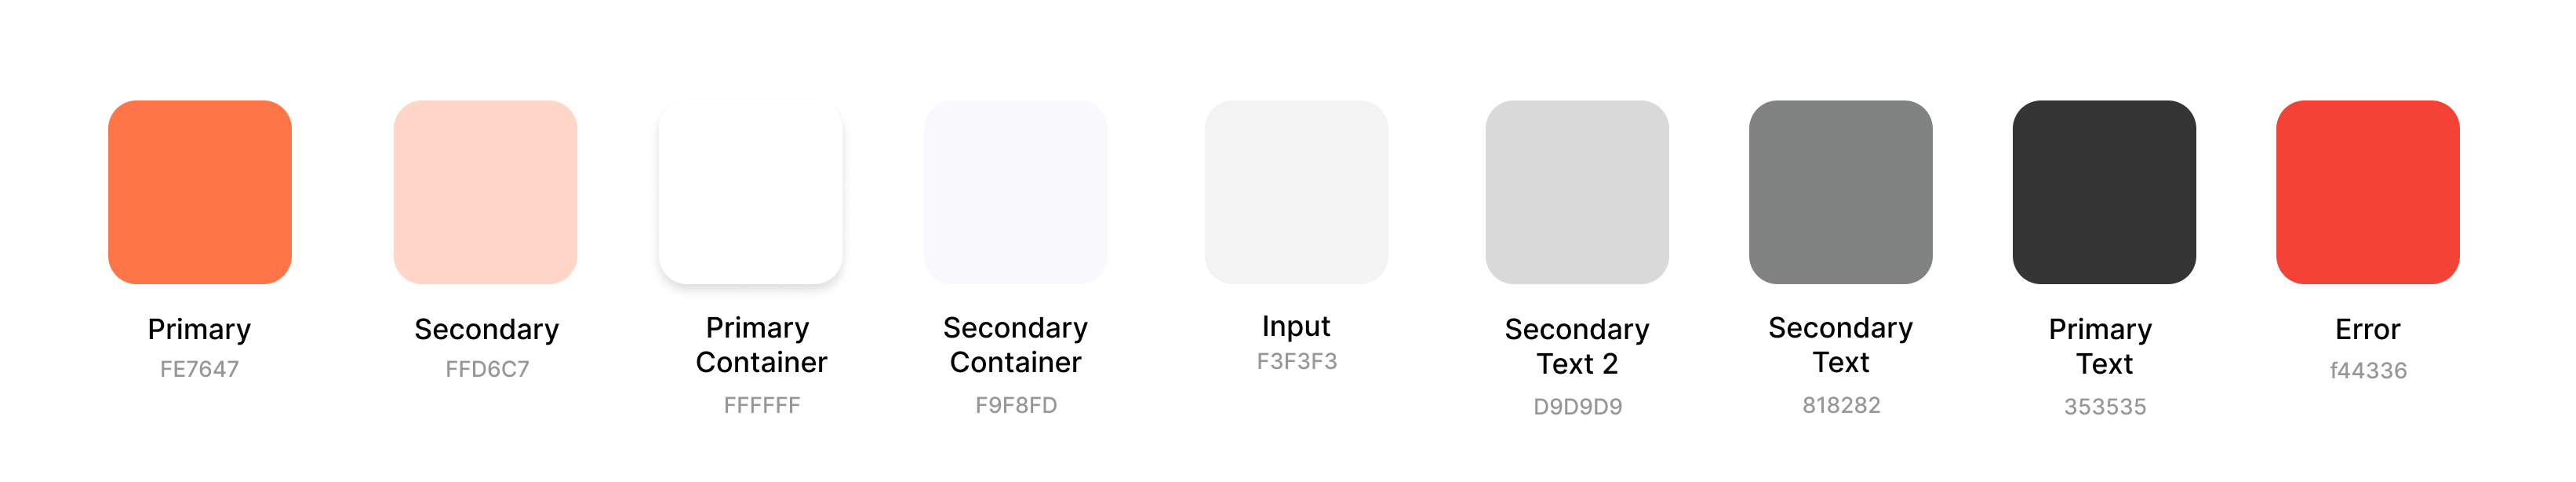
\includegraphics[width=1\textwidth]{pics/colors.png}
  \caption{Nochba Farbpalette}
  \label{fig:color-chart}
\end{figure}

Bevor der endgültige Farbton ausgewählt wurde, wurden verschiedene orangefarbene Töne für den Prototypen ausprobiert und für einige Tage beobachtet, um ein Gefühl für die Farbe zu bekommen. Schließlich wurde sich für die endgültigen Farben entschieden, wie in der Abbildung \ref{fig:color-chart} dargestellt.

Die Hauptcontainerfarbe für die meisten Ansichten ist Weiß, ebenso wie die Hintergrundfarbe der Posts. Allerdings wurde eine Farbe gesucht, die gut als Hintergrund passt, weshalb ein helles Grau verwendet wurde.

Für die Textfarbpalette wurde fast Schwarz gewählt, da dies zu einem weicheren Eindruck führt. Um Untertitel weniger präsent zu gestalten, wurde ein etwas hellerer Grauton gewählt.


\subsubsection{Icons}


\begin{figure}[ht]
  \centering
  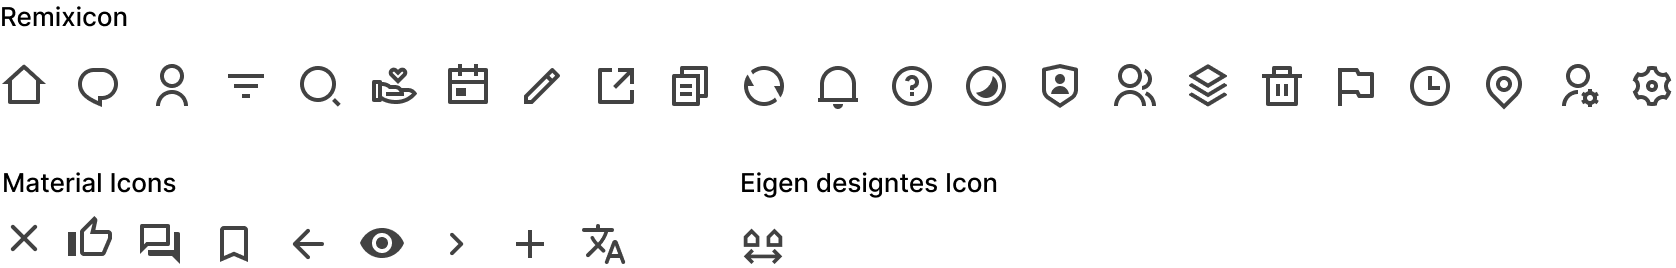
\includegraphics[width=1\textwidth]{pics/icons.png}
  \caption{App Icons}
  \label{fig:app-icons}
\end{figure}

Die obige Abbildung \ref{fig:app-icons} zeigt alle Icons,
die in einer App verwendet werden. Das Ziel war es, eine
möglichst große Anzahl von Icons zu integrieren, um die
Benutzerfreundlichkeit und Bedienbarkeit der App zu
verbessern.

Nachdem verschiedene Icon-Packs betrachtet wurden, wurde hauptsächlich das frei verfügbare Remixicon-Pack\cite{remixicon} verwendet, um der App ein einzigartiges Aussehen zu verleihen und sie von anderen Apps abzuheben. Das runde Design der Icons wurde besonders geschätzt. Ein weiterer Vorteil von Remixicons ist, dass es ein Flutter-Package\cite{remixicon_flutter_package} gibt, was die Implementierung erleichtert hat.

Obwohl Remixicons viele Icons zur Verfügung stellt, wurden bei einigen Icons die Material Icons\cite{material_icons} von Google bevorzugt.

Insbesondere die abgerundeten Icons wurden verwendet, um das
Design insgesamt weicher zu gestalten. Da kein passendes
Icon vorhanden war, um den Abstand zwischen zwei Nachbarn zu
symbolisieren, wurde ein neues Icon im Stil der anderen
entworfen.

\subsubsection{Typografie}
\begin{figure}[H]
  \centering
  
\includegraphics[width=1\textwidth]{pics/font.png}
  \caption{Die Schriftfamilie Inter}
  \label{fig:font}
\end{figure}

Ein wichtiger Teil jedes Designs ist die Typografie, so auch bei der Nochba-App.

Der Designer der App war auf der Suche nach einer
Schriftart, die modern, ansprechend und gut lesbar ist. Er
suchte nach einer Schriftart, die Lesbarkeit und das
Verständnis des Textes verbessert. Schließlich stieß er auf
die Schriftart 'Inter' von Rasmus Andersson
\cite{inter-font}, die man auf der Abbildung \ref{fig:font}
betrachten kann.

Inter ist eine moderne und ansprechende Schriftart, die speziell für die Verwendung auf Bildschirmen entwickelt wurde. Die Schriftart ist in vielen verschiedenen Stilen verfügbar und bietet eine breite Unterstützung für verschiedene Sprachen und Schriftsysteme. Dies war besonders wichtig für den Designer der Nachbarschafts-App, da die App von Menschen aus verschiedenen Ländern genutzt wird, die möglicherweise unterschiedliche Sprachen und Schriftsysteme verwenden.

Ein weiterer Vorteil von Inter ist seine Lesbarkeit. Die Schriftart ist gut lesbar, auch in kleineren Größen, was besonders wichtig ist, da die App oft auf mobilen Geräten verwendet wird. Die klare und prägnante Schriftart von Inter verbessert auch die Lesbarkeit und das Verständnis des Textes, was wiederum zu einer besseren Benutzererfahrung führt.

Schließlich ist Inter auch eine Open-Source-Schriftart, die kostenlos verwendet werden kann \cite{inter-font}. Dies ist besonders wichtig für das Projekt Nochba, da Nochba für Open Source Stehen will.

Zusammenfassend lässt sich sagen, dass Inter eine ausgezeichnete Wahl für die Nachbarschafts-App ist. Die Schriftart ist modern, ansprechend und gut lesbar, und bietet eine breite Unterstützung für verschiedene Sprachen und Schriftsysteme. Die Verwendung von Inter hat dem Designer der App geholfen, eine professionelle und kosteneffektive Lösung für die Entwicklung der App zu finden.
\subsubsection{Logo}

\begin{figure}[H]
  \centering
  
\includegraphics[width=0.95\textwidth]{pics/final-logo.png}
  \caption{Finales Logo}
  \label{fig:final-logo}
\end{figure}

% 
\includegraphics[width=0.35\textwidth]{pics/app-logo.png}

% überschrift logo historie
\paragraph{Logo Historie}\mbox{} \\
% \hspace*{\parindent}


Im Zuge des Designprozesses wurden hohe Ansprüche an das
Logo der App gestellt, da es das Projekt repräsentiert und
es dem Team wichtig ist. Es
war wichtig, dass das Logo einfach gehalten und leicht
erkennbar ist.

\begin{figure}[H]
  \centering
  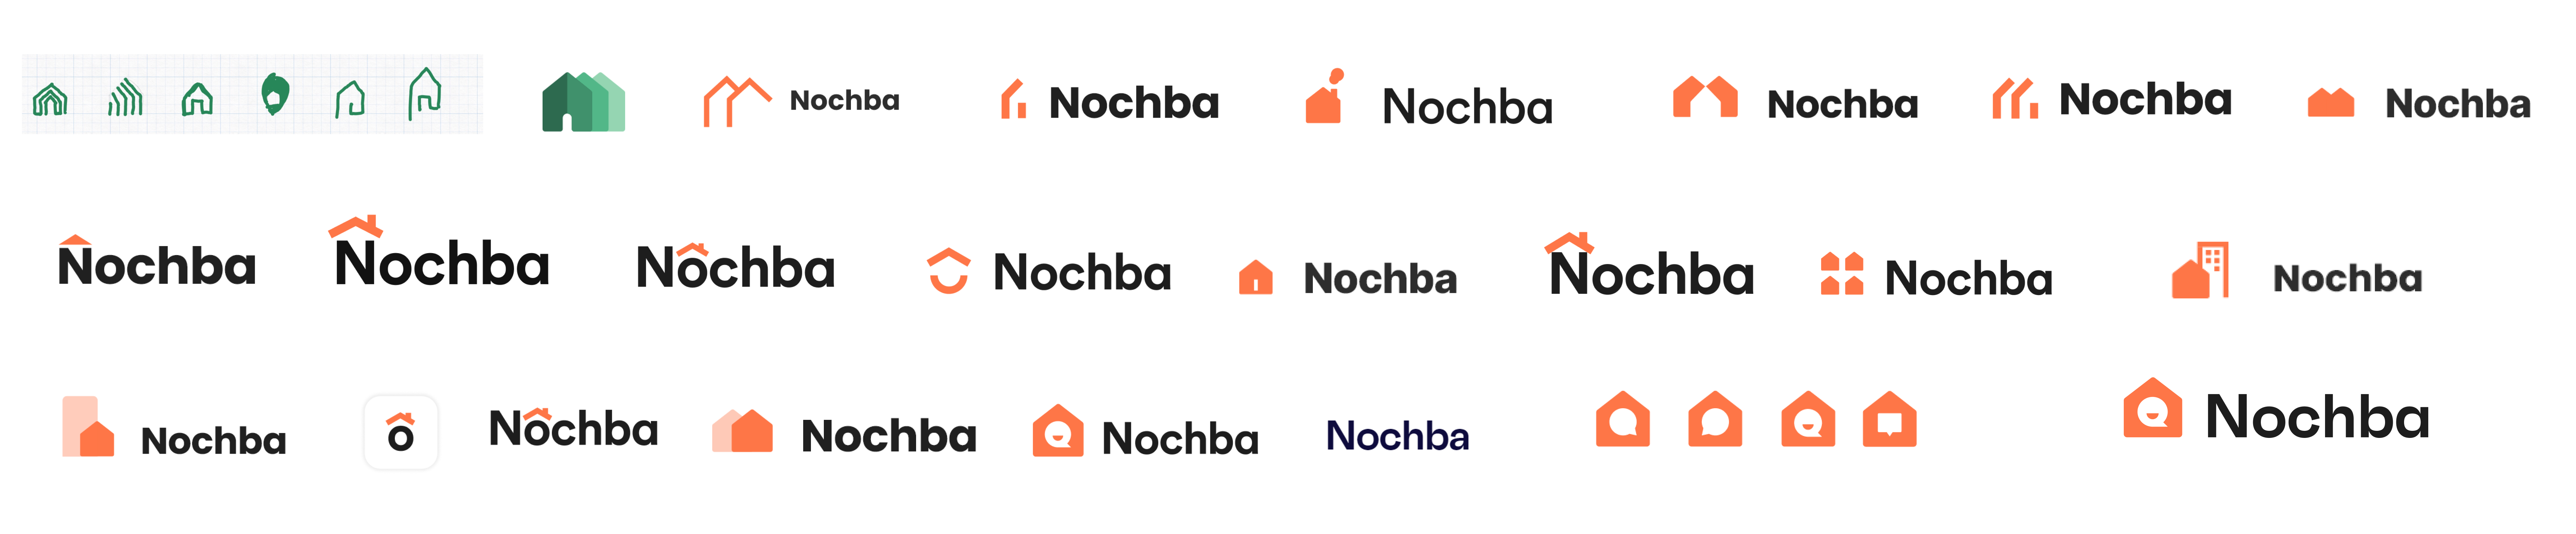
\includegraphics[width=0.95\textwidth]{pics/logo-historie.png}
  \caption{Logo Design Ideen}
  \label{fig:logo-historie}
\end{figure}

Die endgültige Gestaltung des Logos hat viel Zeit
in Anspruch genommen, da die vorherigen Entwürfe nicht
vollständig zufriedenstellten die man bei Abbildung
\ref{fig:logo-historie} sieht. Nach anderen Logos, die eine
Verbindung zu Nachbarschaften oder Häusern herstellen, wurde
gezielt gesucht und Ideen auf dem Discord-Server
gespeichert. Es sollte immer ein Haus erkennbar sein, da
Häuser schnell mit Nachbarschaften in Verbindung gebracht
werden.

In den früheren Versionen der App gab es Schwierigkeiten,
ein ansprechendes App-Icon zu gestalten, da kein
eigenständiges Icon vorhanden war. Aus diesem Grund wurde
entschieden, den Schriftzug und das App-Icon (Logo) separat
zu gestalten, wie es auch bei anderen Apps üblich ist. Das
endgültige Logo wurde erst Ende 2022 entworfen, da alle
anderen Designs nicht gefielen. Es wurde ein Haus mit einer
sprechenden Sprechblase, die lächelt, als Logo
wie bei Abbildung \ref{fig:final-logo} zu sehen ist gewählt. Dies soll symbolisieren, dass
man innerhalb des Hauses sprechen kann und das Lächeln soll
verdeutlichen, dass man Freude mit seinen Nachbarn teilen
kann. Eine runde, verspieltere Schriftart wurde bewusst
gewählt, da sie besser mit der Farbmischung harmoniert als
die vorherige Schriftart.



\subsection{App Design}
\subsubsection{Thumb Zone Prinzip}
\setauthor{Martin Hausleitner}

\begin{figure}[h]
  \centering
  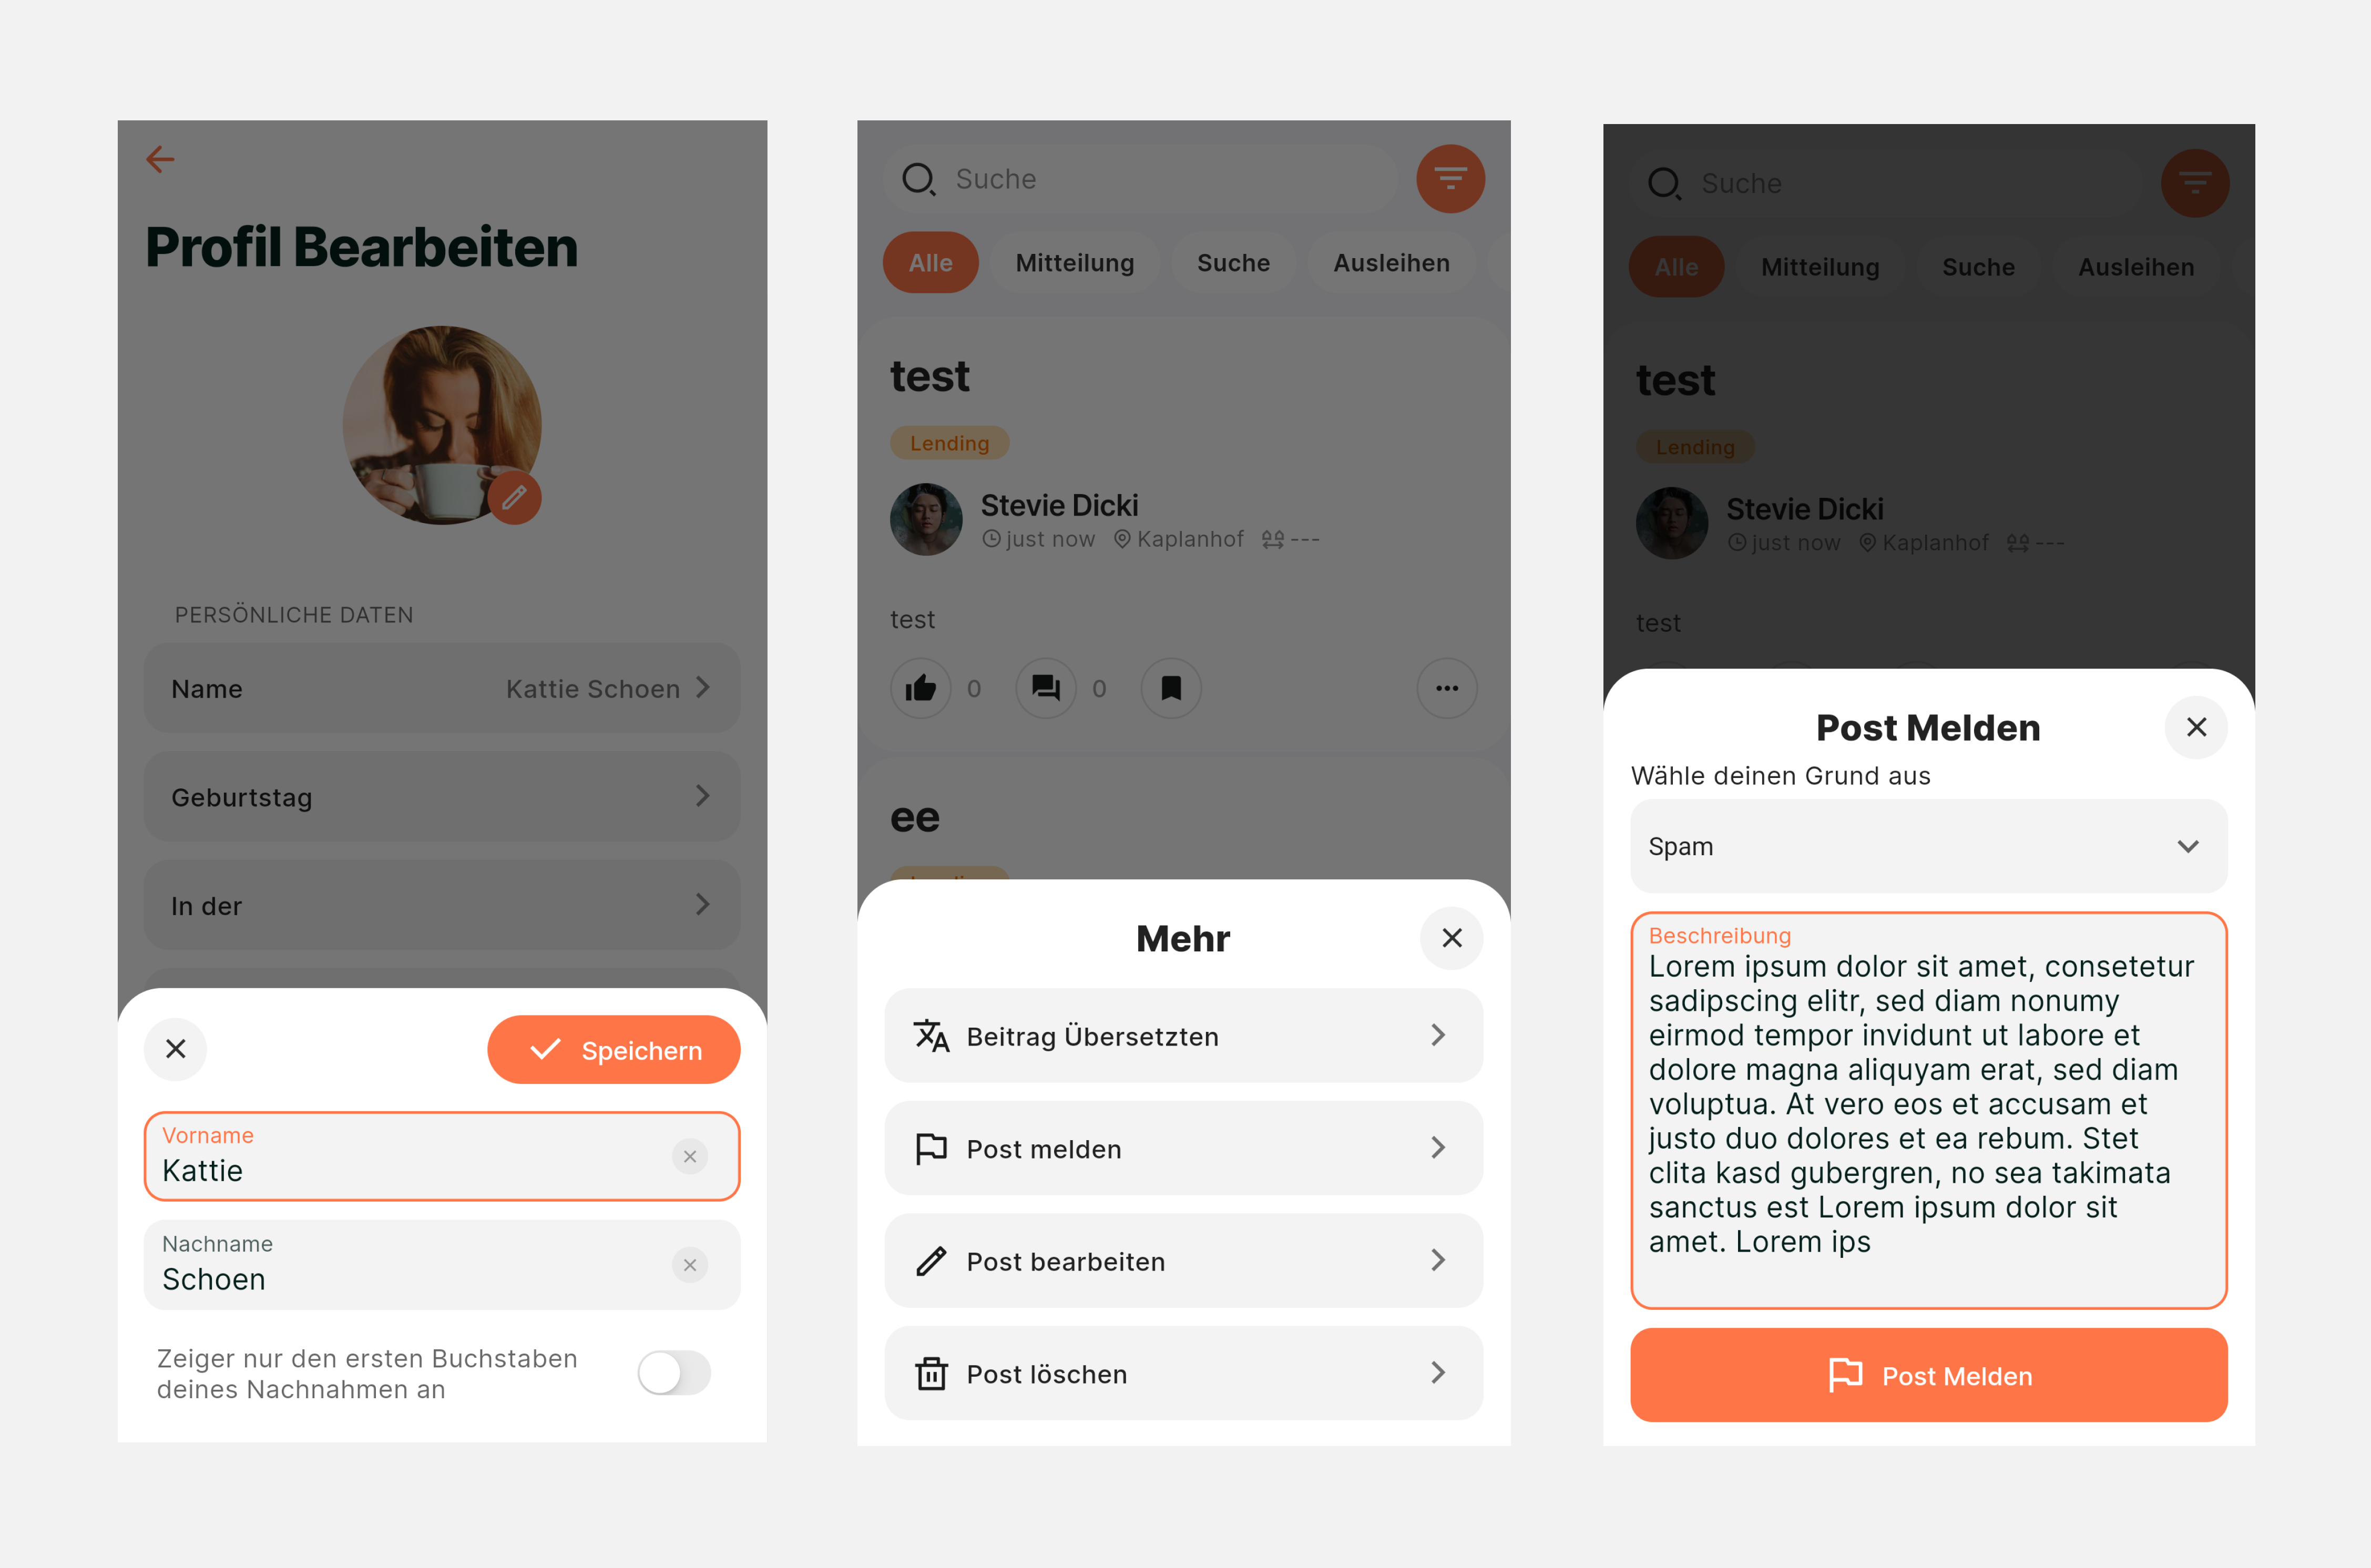
\includegraphics[width=1\textwidth]{pics/thumb-zone.png}
  \caption{Abbildung mehere Thumbs Zones in der App}
  \label{fig:thumb-zone}
\end{figure}

% \begin{figure}[h]
%   \centering
%   \begin{minipage}[b]{0.3\textwidth}
%     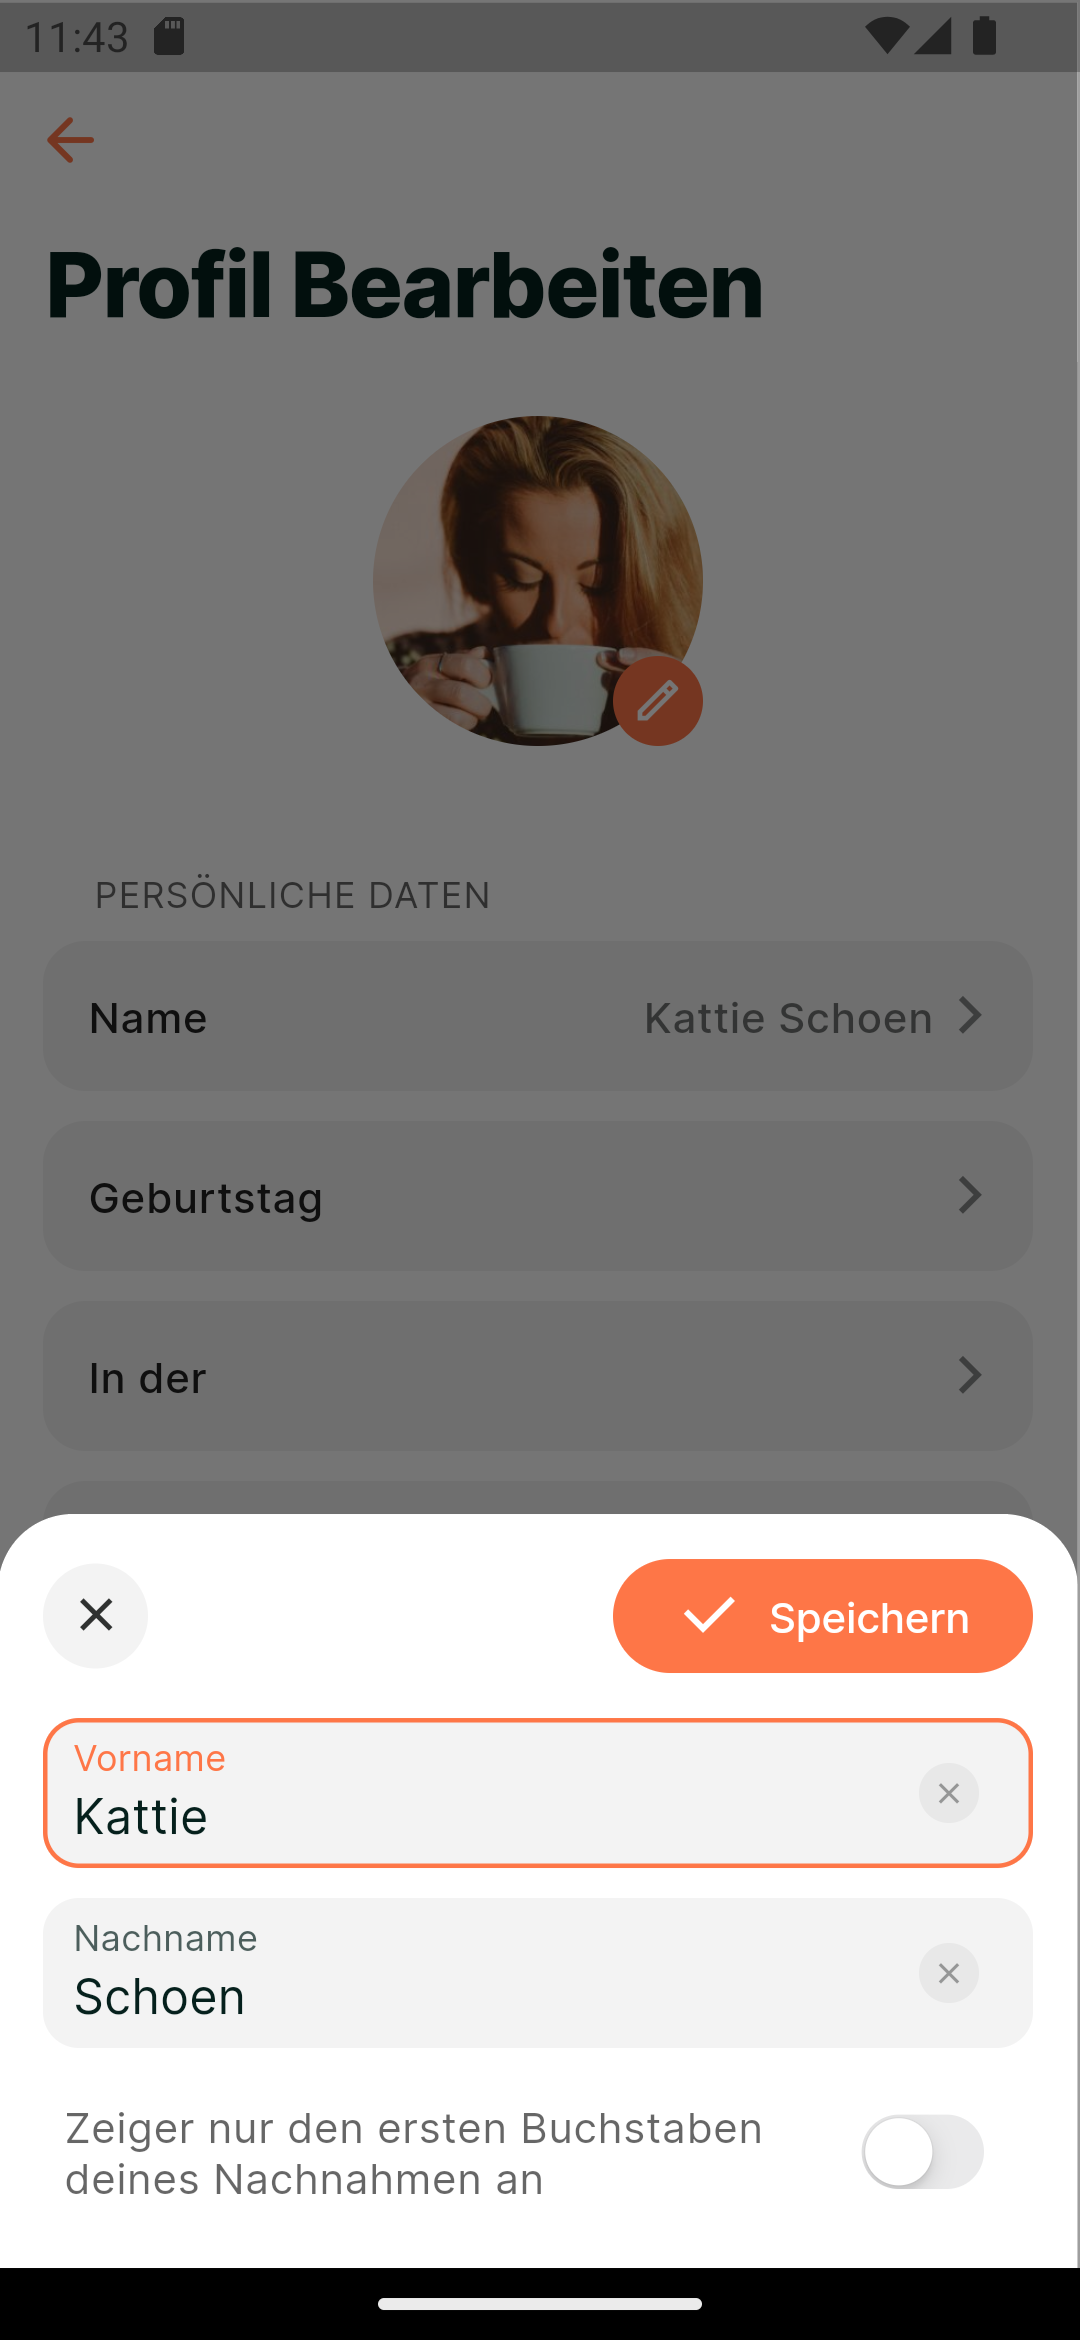
\includegraphics[width=\textwidth]{pics/edit-name-screen.png}
%     \caption{Screenshot des 'Name bearbeiten'-Screens}
%     \label{fig:edit-name-screen}
%   \end{minipage}
%   \hfill
%   \begin{minipage}[b]{0.3\textwidth}
%     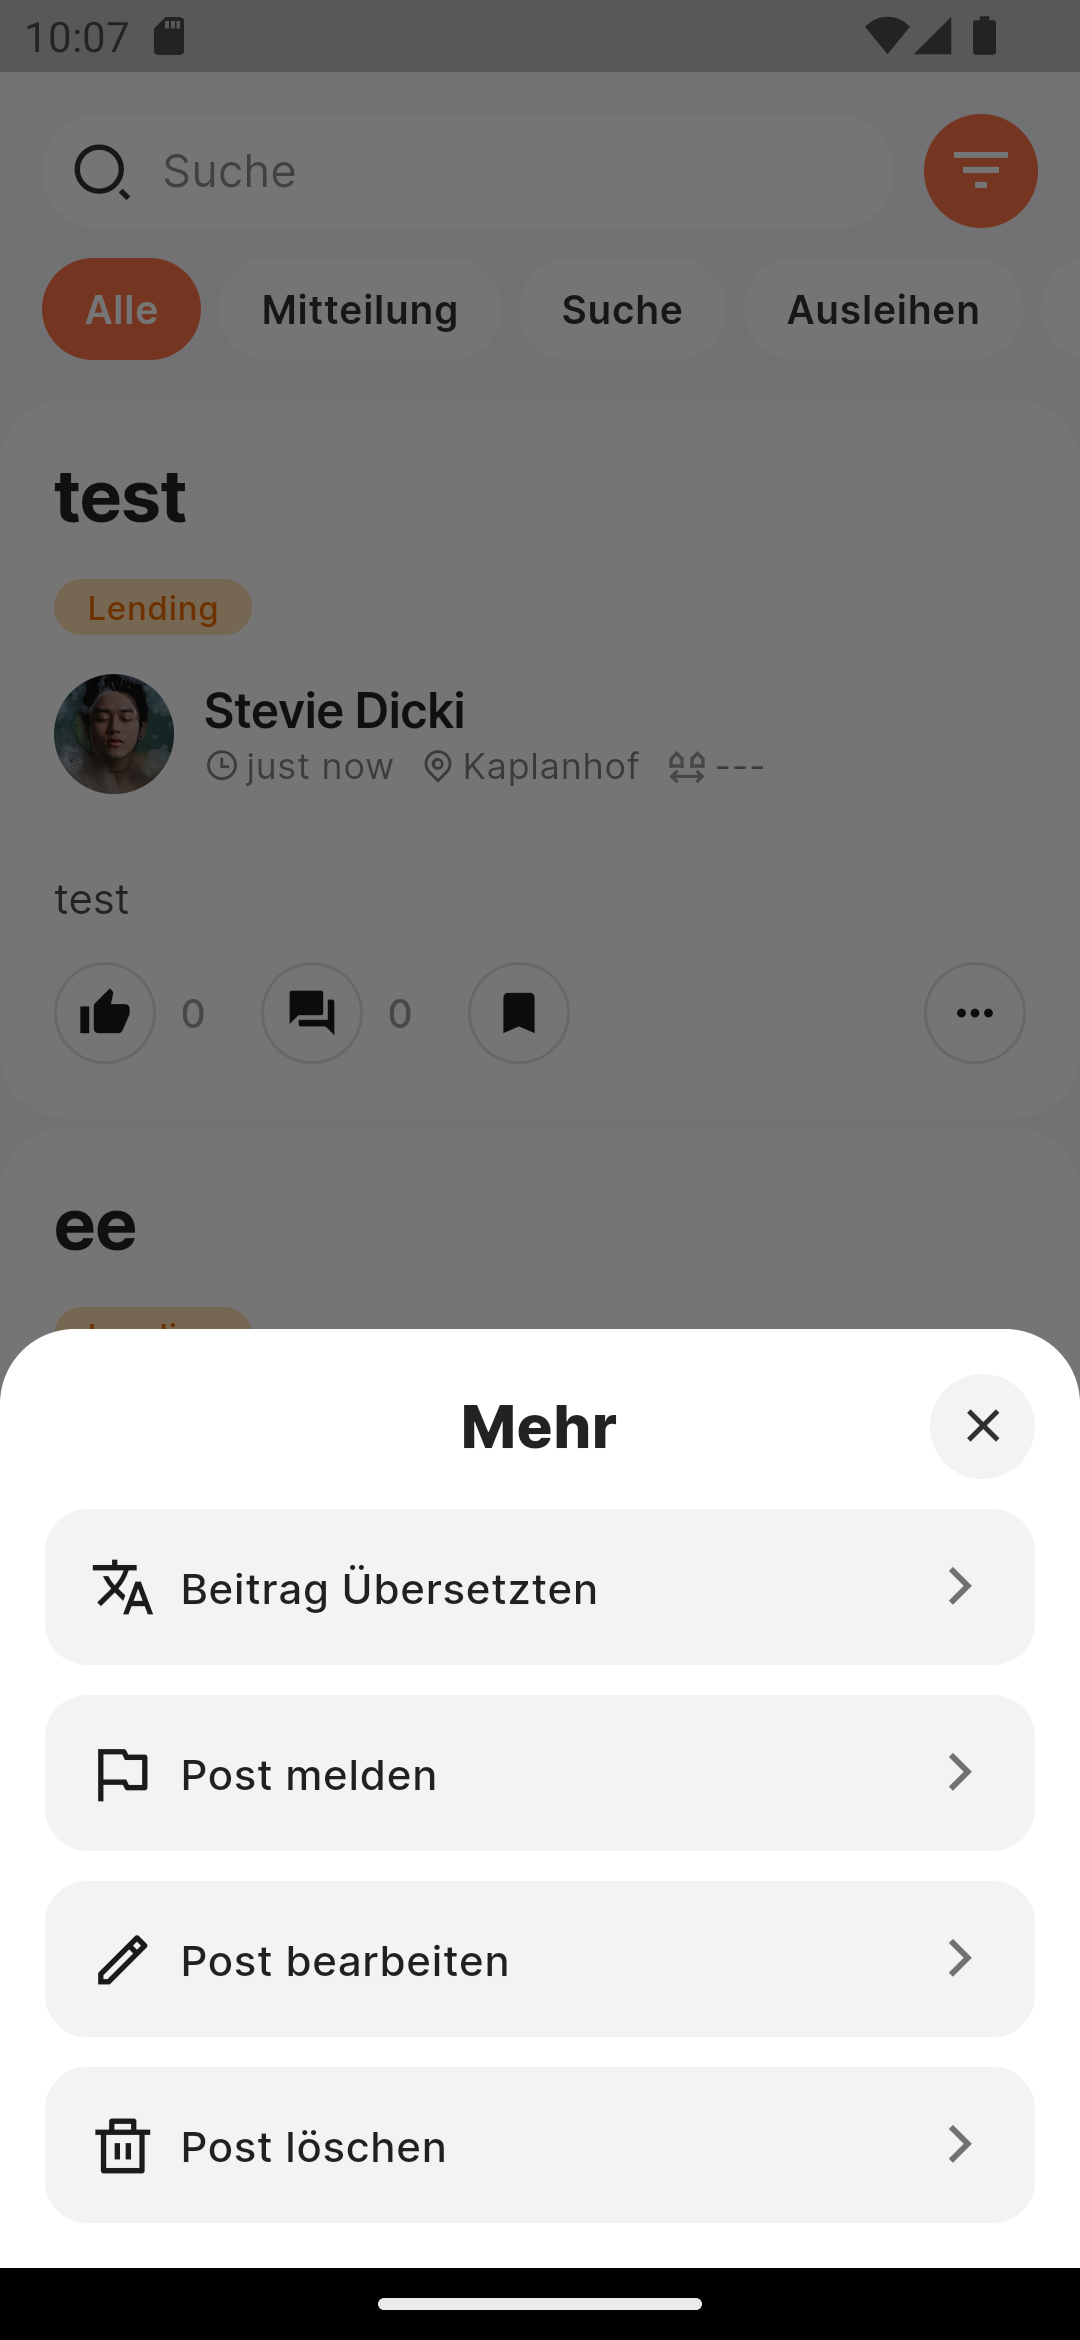
\includegraphics[width=\textwidth]{pics/post-more-menu.png}
%     \caption{Screenshot des 'Mehr'-Menüs für Beiträge}
%     \label{fig:post-more-menu}
%   \end{minipage}
%   \hfill
%   \begin{minipage}[b]{0.3\textwidth}
%     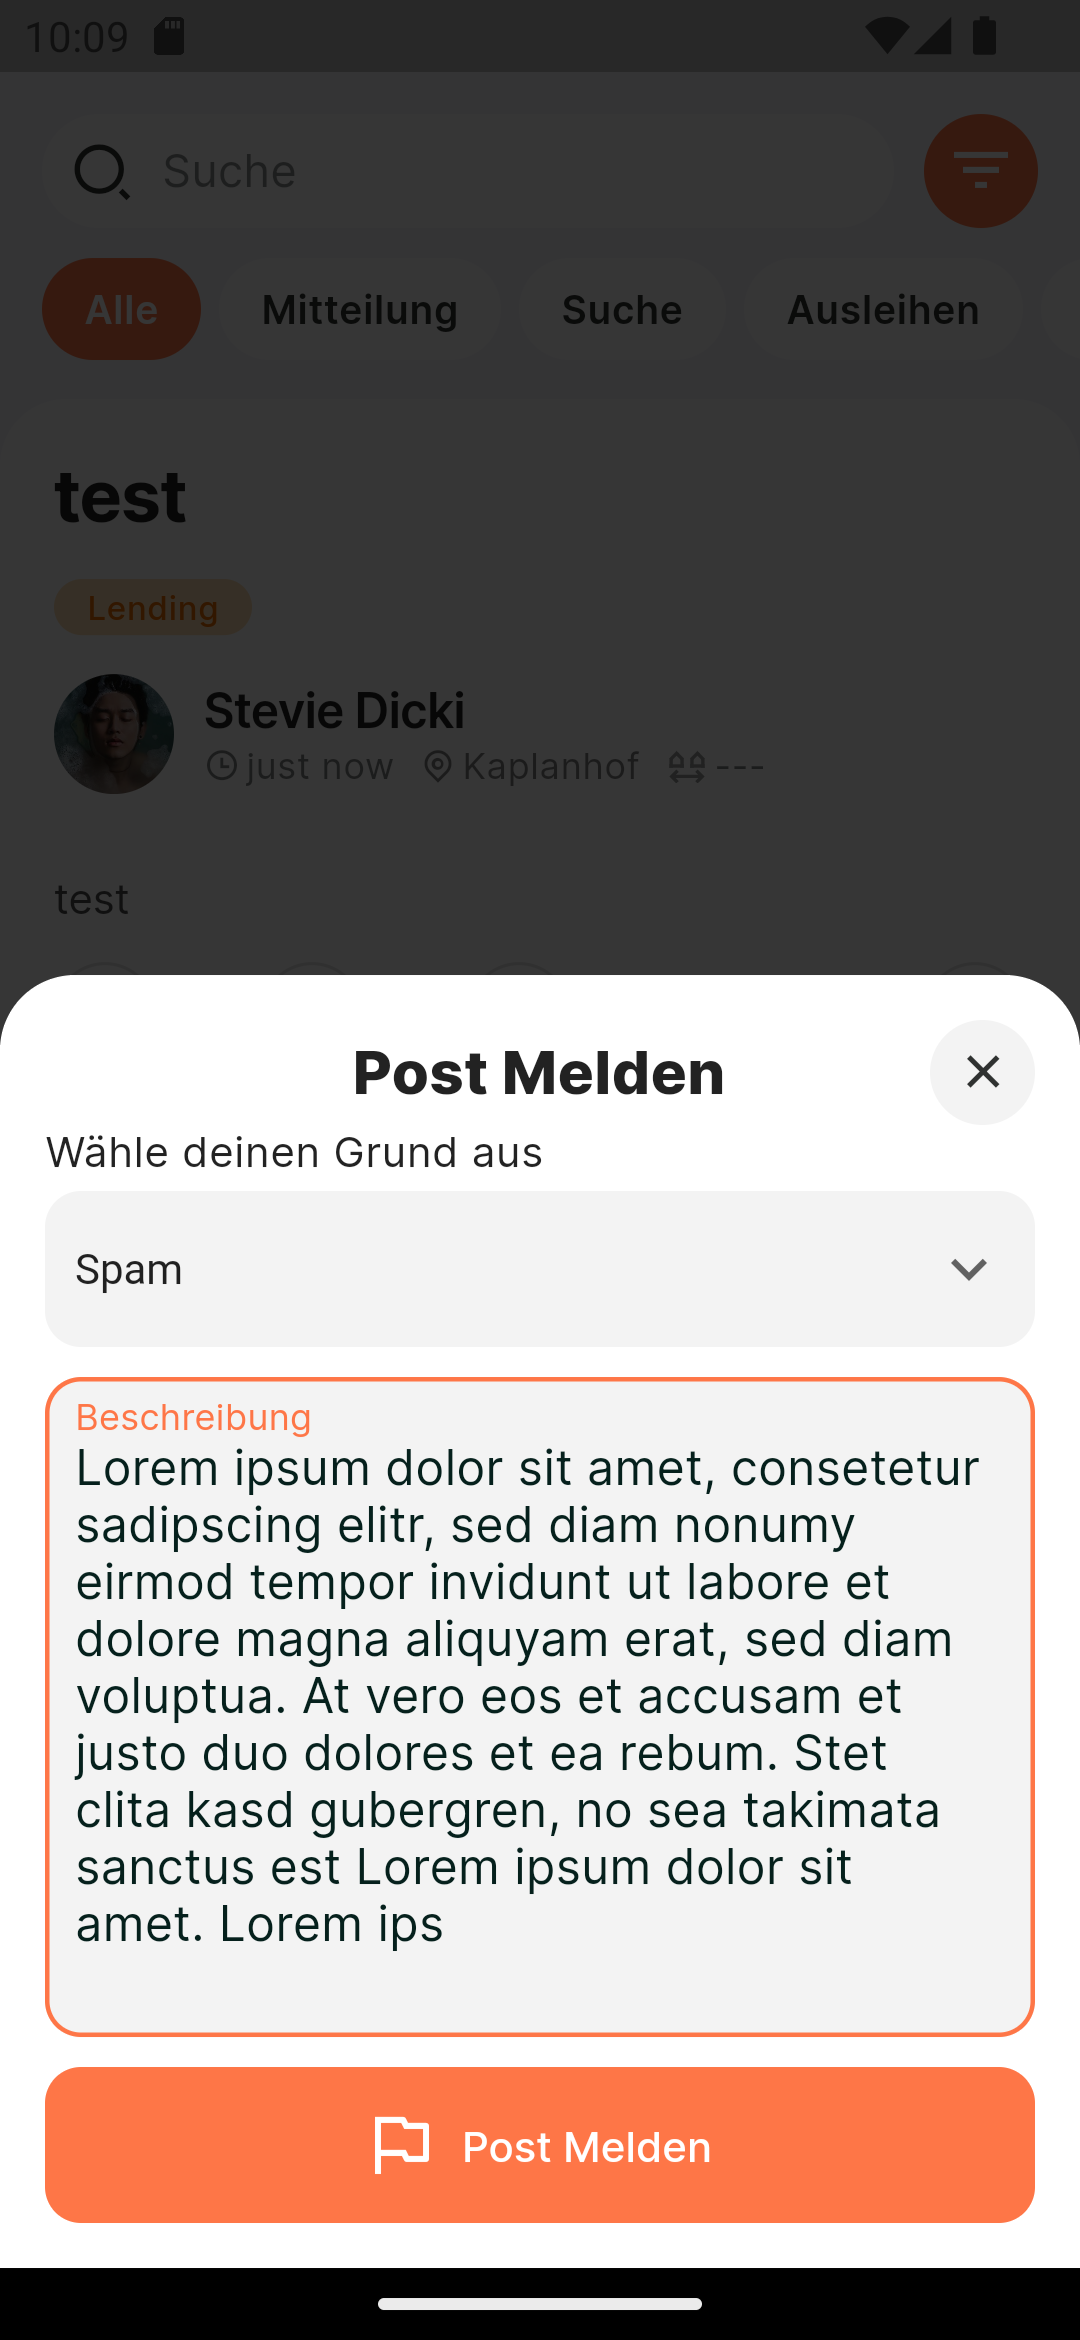
\includegraphics[width=\textwidth]{pics/post-report-menu.png}
%     \caption{Screenshot des 'Beitrag melden'-Menüs}
%     \label{fig:post-report-menu}
%   \end{minipage}
% \end{figure}
Im Design-Muster wurde versucht, das Thumb Zone Prinzip zu
implementieren, indem wichtige UI-Elemente immer im unteren
Bereich der App platziert wurden. Das Layout für die
Namensbearbeitung \ref{fig:thumb-zone} wurde extra
unten platziert, um alle Klick-Elemente bequem mit dem
Daumen bedienen zu können. Wichtige
wie 'Speichern'
wurden in der primären Farbe gestaltet und rechts
ausgerichtet, um einen leichteren Zugriff zu gewährleisten.
Das Textfeld kann einfach durch Drücken der Enter-Taste auf
der Tastatur geändert werden, um das Eintippen von Daten zu
erleichtern.

Wie bei Abbildung \ref{fig:thumb-zone} zu sehen ist, erfolgt eine weitere Implementierung einer Bottom View, um dem Thumb Zone Prinzip gerecht zu werden.

Unwichtige Buttons wurden in grau gestaltet, wie z.B. der X-Button in der Abbildung. Ein Löschen-Button neben dem Textfeld wurde eingebaut, der es dem Benutzer ermöglicht, den gesamten Text bequem zu löschen. Jedoch war es nicht möglich, diese Prinzipien vollständig umzusetzen, da die Zeit gegen Ende knapp wurde. In zukünftigen Versionen der App soll sichergestellt werden, dass diese Prinzipien einheitlich angewendet werden.
\subsubsection{Design Historie}

\begin{figure}[h]
  \centering
  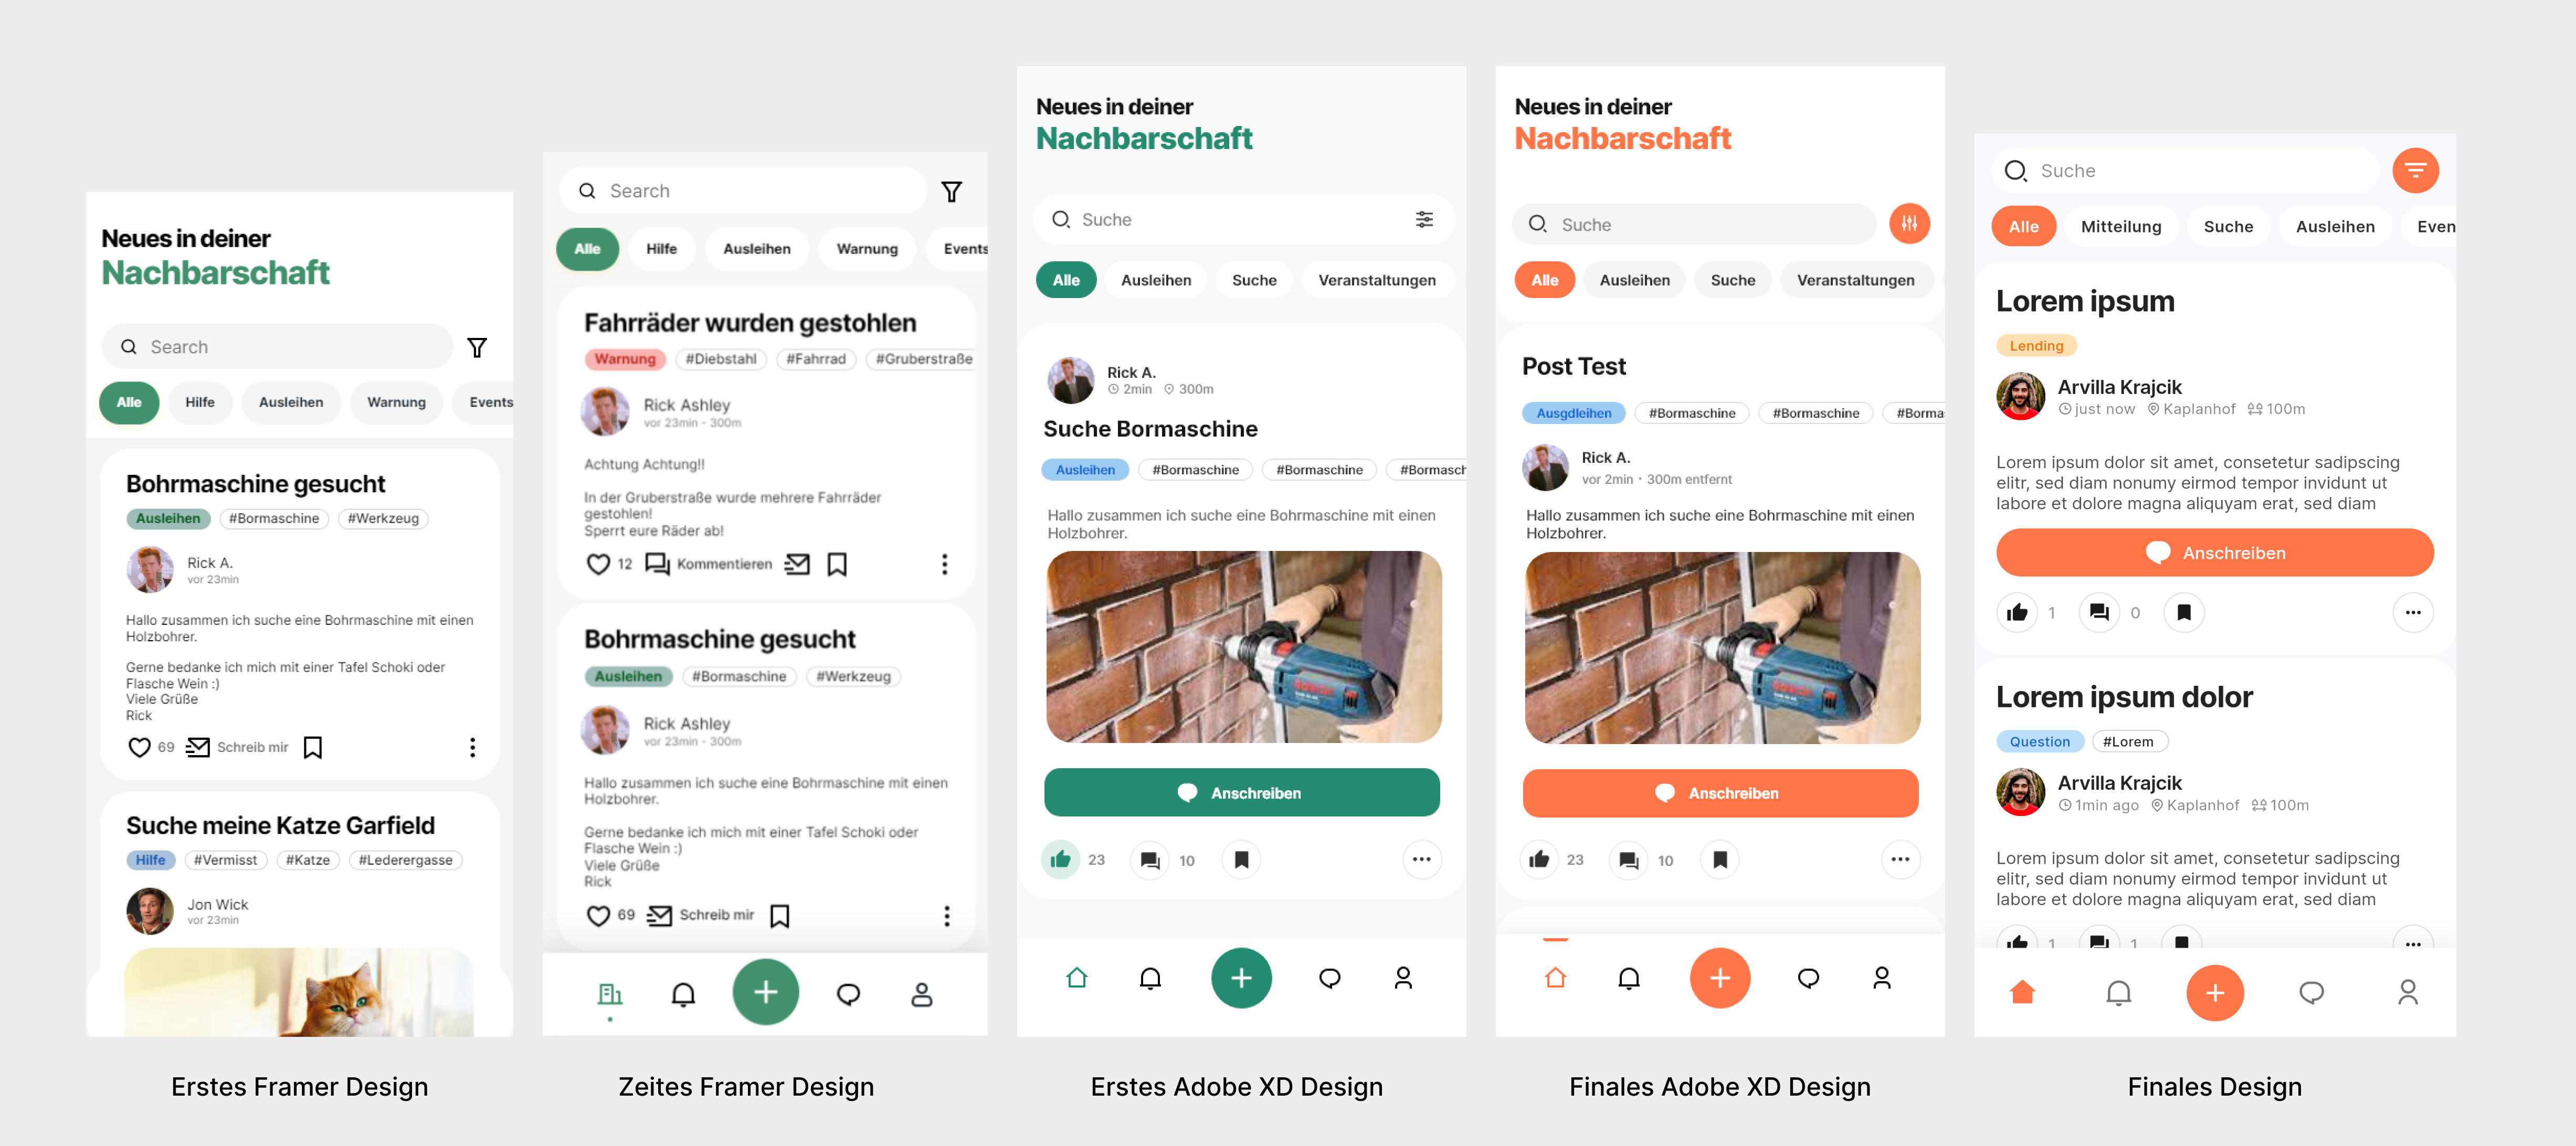
\includegraphics[width=1\textwidth]{pics/app-design-history.png}
  \caption{Screenshots verschiedener Versionen des App-Home-Screen}
  \label{fig:app-design-history}
\end{figure}
Im Rahmen des Hackathons Linz hACkT wurde das erste Design in Abbildung \ref{fig:app-design-history} ganz links erstellt. Hierbei wurden mehrere Brainstorming-Meetings mit Mentoren abgehalten, um ein Grundkonzept in Adobe XD zu gestalten. Anschließend wurden die groben Züge des Designs in Absprache mit dem Team festgelegt. Ein funktionsfähiger Prototyp wurde in Framer erstellt und am Tag der Endpräsentationen vorgestellt und verlinkt. Nach Linz haCKt wurde das zweite Design in Framer entwickelt.

Zwischen dem zweiten Framer-Design
\ref{fig:app-design-history} und dem ersten Adobe XD-Design
\ref{fig:app-design-history} wurde bewusst kein Abstand am
Rand eines Beitrags gehalten, um den vollen Handy-Display
auszunutzen. Der Filter-Button wurde mit der Suchleiste
verbunden, um das Design stimmiger zu gestalten. Bei den
Profilinformationen wurde auf Icons umgestellt, um es für
neue Nutzer verständlicher zu machen. Diese Entscheidung
wurde kurzzeitig verworfen, jedoch später in der Flutter-App
wieder eingebaut.

Wie man erkennen kann, wurde für das Finale Adobe
XD-Design \ref{fig:app-design-history} eine orangene Farbe für die Kapitelfarben
gewählt. Der letzte Screenshot zeigt die Flutter-App, wie
sie im Play Store erhältlich ist. Die größte Änderung
gegenüber dem vorherigen Design betrifft den Hintergrund
bei der Suche und der Kategorieauswahl. Der Hintergrund
wurde hellgrau gemacht, um die Beiträge besser hervorzuheben.
Bei der Entwicklung mit Flutter stellte sich heraus, dass
ein Strich über dem aktiven Icon sehr aufwändig zu
implementieren ist, weshalb darauf verzichtet wurde.




\section{Website}
\setauthor{Martin Hausleitner}
\begin{figure}[h]
  % \centering
  
\includegraphics[width=1\textwidth]{pics/website-design.png}
  \caption{Screenshot der Nochba Website: nochba.at}
\end{figure}

Die Medienpräsenz des Projekts, die durch die Teilnahme an
Linz hACkT erlangt wurde, und das Fehlen eines zentralen
Anlaufpunkts für Informationen führten zur Entscheidung,
eine einfache Landing Page zu erstellen.
Diese Seite bietet grundlegende Informationen und ist unter nochba.at\cite{nochba_at} erreichbar.

Die Teilnahme am mPreneur Social Mobile Entrepreneurship von Arsham Edalatkhah führte zu internationaler Aufmerksamkeit für das Projekt. Dies veranlasste die Erstellung einer englischsprachigen Website unter nochba.com\cite{nochba_com}.



Ziel ist es, die Arbeit einem breiteren Publikum zugänglich zu machen und die Reichweite des Projekts zu erhöhen. Durch die Präsenz in einer internationalen Sprache kann das Interesse von Menschen aus verschiedenen Ländern und Kulturen geweckt und potenziell eine größere Nutzerbasis erreicht werden.


\subsection{Beta-tester anmeldung}
Das wichtigste Merkmal der Website ist die Option für Nutzer, sich für die Testphase zu registrieren. Ursprünglich wurde versucht, die E-Mail-Adressen der Nutzer über die Google Sheets API zu speichern. Allerdings erwies sich dieser Ansatz als ineffektiv und dauerte mehrere Stunden. Als Alternative wurde das Framer-Add-On von Mailchimp.com genutzt, um Zeit zu sparen. Der kostenlose Plan von Mailchimp war für die Bedürfnisse ausreichend. Stand 7.3.2023 wurden 34 Beta-Anmeldungen über das Formularfeld gesammelt.


\subsection{Design}
Für die Gestaltung der Landing Page ließ sich der Designer
von den Vorlagen von Framer inspirieren und nutzte
vorgefertigte Abschnitte. Diese wurden jedoch so
modifiziert, dass sie dem Designsysten gerecht werden. Die
Farbpalette wurde beibehalten und es wurde darauf geachtet,
dass die Website möglichst einfach gestaltet ist.

\subsection{Kontent}
Auf der Website sind folgende Informationen abgebildet:
\begin{itemize}
  \item Zeitungsartikel
        \begin{itemize}
          \item Mein Bezirk\cite{mein_bezirk}
          \item Linz\cite{linz}
          \item OÖNachrichten\cite{oo_nachrichten}
          \item DorfTV\cite{dorf_tv}
          \item Kronen Zeitung (nur auf Papier)
        \end{itemize}
  \item Unsere Mission
  \item Beitrag Kategorien
  \item Auszeichnungen
        \begin{itemize}
          \item Immotopia Innovation Award
          \item mPreneur Austria
          \item Linz hACkt
        \end{itemize}
  \item Features der App
  \item Partner der Diplomarbeit
  \item Über uns
  \item Links
        \begin{itemize}
          \item Github Repo\cite{github_repo}
          \item Instagram\cite{nochba_instagram}
          \item Email \href{mailto:project@nochba.com}{project@nochba.com}
        \end{itemize}
\end{itemize}



\subsection{Hosting}
Die Website wurde mithilfe von \cite{framer} erstellt und auf deren
Hosting-Plattform gehostet. Um die Domain-Namen zu nutzen,
die über \cite{godaddy} (nochba.at und nochba.com) gekauft wurden, wurde eine Weiterleitung
mit Maskierung auf die entsprechende Framer-URL
eingerichtet. Durch diese Maßnahme wurde im Browser bei der
URL die gekaufte Domain angezeigt.


\subsubsection{SSL-Zertifikat}
Aktuell verfügt die Website über kein SSL-Zertifikat, da durch die Maskierung das Framer SSL-Zertifikat entfällt. Dennoch wird die Website im Browser nicht als bedrohlich eingestuft. Aus diesem Grund wurde entschieden, kein SSL-Zertifikat zu erstellen und somit den Aufwand zu reduzieren.

\section{Backend}


\subsection{Firebase}
\setauthor{Martin Hausleitner}
Firebase ist ein Backend-as-a-Service (BaaS), das Entwicklern eine enorme Erleichterung bei der Arbeit bietet. Das Hosting von Datenbanken und Cloud-Funktionen kann mit nur wenigen Klicks erfolgen, was die Notwendigkeit von Skalierung oder Ausfallvermeidung eliminiert. Das Firebase-Backend wird auf der Google Cloud in Frankfurt (EUR3 Europe-West) gehostet, um eine niedrige Latenz zu gewährleisten. Der kostenlose Spark-Plan war für den Gebrauch ausreichend, als der Dienst noch nicht die Firebase-Cloud-Funktionen genutzt hat. Um Kosten zu sparen, wurde lange Zeit mit dem Firebase-Emulator an den Cloud-Funktionen gearbeitet. Im Januar 2023 wurde auf den Blaze-Plan umgestiegen, um die Firebase-Cloud-Funktionen nutzen zu können. Bis März 2022 wurden nur wenige Euro für den Verbrauch gezahlt. Die Dokumentation und Tutorials von Firebase sind exzellent und es gibt viele Ressourcen auf YouTube.

\subsection{Firebase Authentication}
\setauthor{Sandin Habibovic}

Firebase Authentication ist ein wichtiger Bestandteil für die Integration von Benutzerauthentifizierung in der Applikation. Die Implementierung dieses Dienstes soll zur Einhaltung der Privatsphäre der User beitragen, indem ein sicherer und zuverlässiger Authentifizierungsmechanismus bereitgestellt wird.
\\
Darüber hinaus ermöglicht der Dienst eine unkomplizierte Integration mit anderen Firebase-Services, wie zum Beispiel Cloud Firestore.
\\
Für die vorliegende Applikation wurden zwei Authentifizierungsmethoden ausgewählt, die über Firebase Authentication bereitgestellt werden: E-Mail und Passwort sowie Google Authentication. Die Wahl dieser beiden Methoden basiert auf ihrer weiten Verbreitung und Akzeptanz unter den Usern. Beide Methoden bieten unterschiedliche Vorteile und ermöglichen den Benutzern, je nach ihren Präferenzen und Anforderungen, eine geeignete Anmeldeoption auszuwählen.


\subsection{Cloud Firestore}
\setauthor{Sandin Habibovic}
Cloud Firestore dient der Anwendung als NoSQL-Datenbank, die eine dokumentbasierte Speicherung von Daten ermöglicht. Dadurch kann das Datenmodell möglichst an die Kriterien der Anwendungen zugeschnitten und trotzdem noch effizient und performant gestaltet werden.
\\
Ein wichtiger Vorteil der Firestore bietet ist, dass Collections und dazugehörige Subcollections erstellt werden können, um damit Daten in hierarchischen Strukturen zu organisieren. Diese Subcollections können verwendet werden, um abhängige Daten in einer einzigen Anfrage abzurufen und damit den Datenzugriff zu optimieren. Darüber hinaus bietet Firestore die Möglichkeit, Daten auf verschiedenen Ebenen zu filtern und zu sortieren, um nur die benötigten Daten abzurufen, was beim Filtern von Beiträge eine große Rolle spielen kann.
\\
Ein weiterer Vorteil ist die Skalierung von Daten auf Firestore, womit die Anwendung mit hohen Nutzerzahlen und großen Datenmengen, wie zum Beispiel dem Abrufen von Beiträgen, zurecht kommen kann.
\\
Außerdem bietet Firestore noch die Möglichkeit an, Daten in Echtzeit zu synchronisieren, um damit auf Änderungen in der Datenbank sofort reagieren zu können und die Applikation somit reaktiv zu halten.


\subsubsection{Datenmodell}
\setauthor{Sandin Habibovic}

\begin{figure}[h]
  \centering
  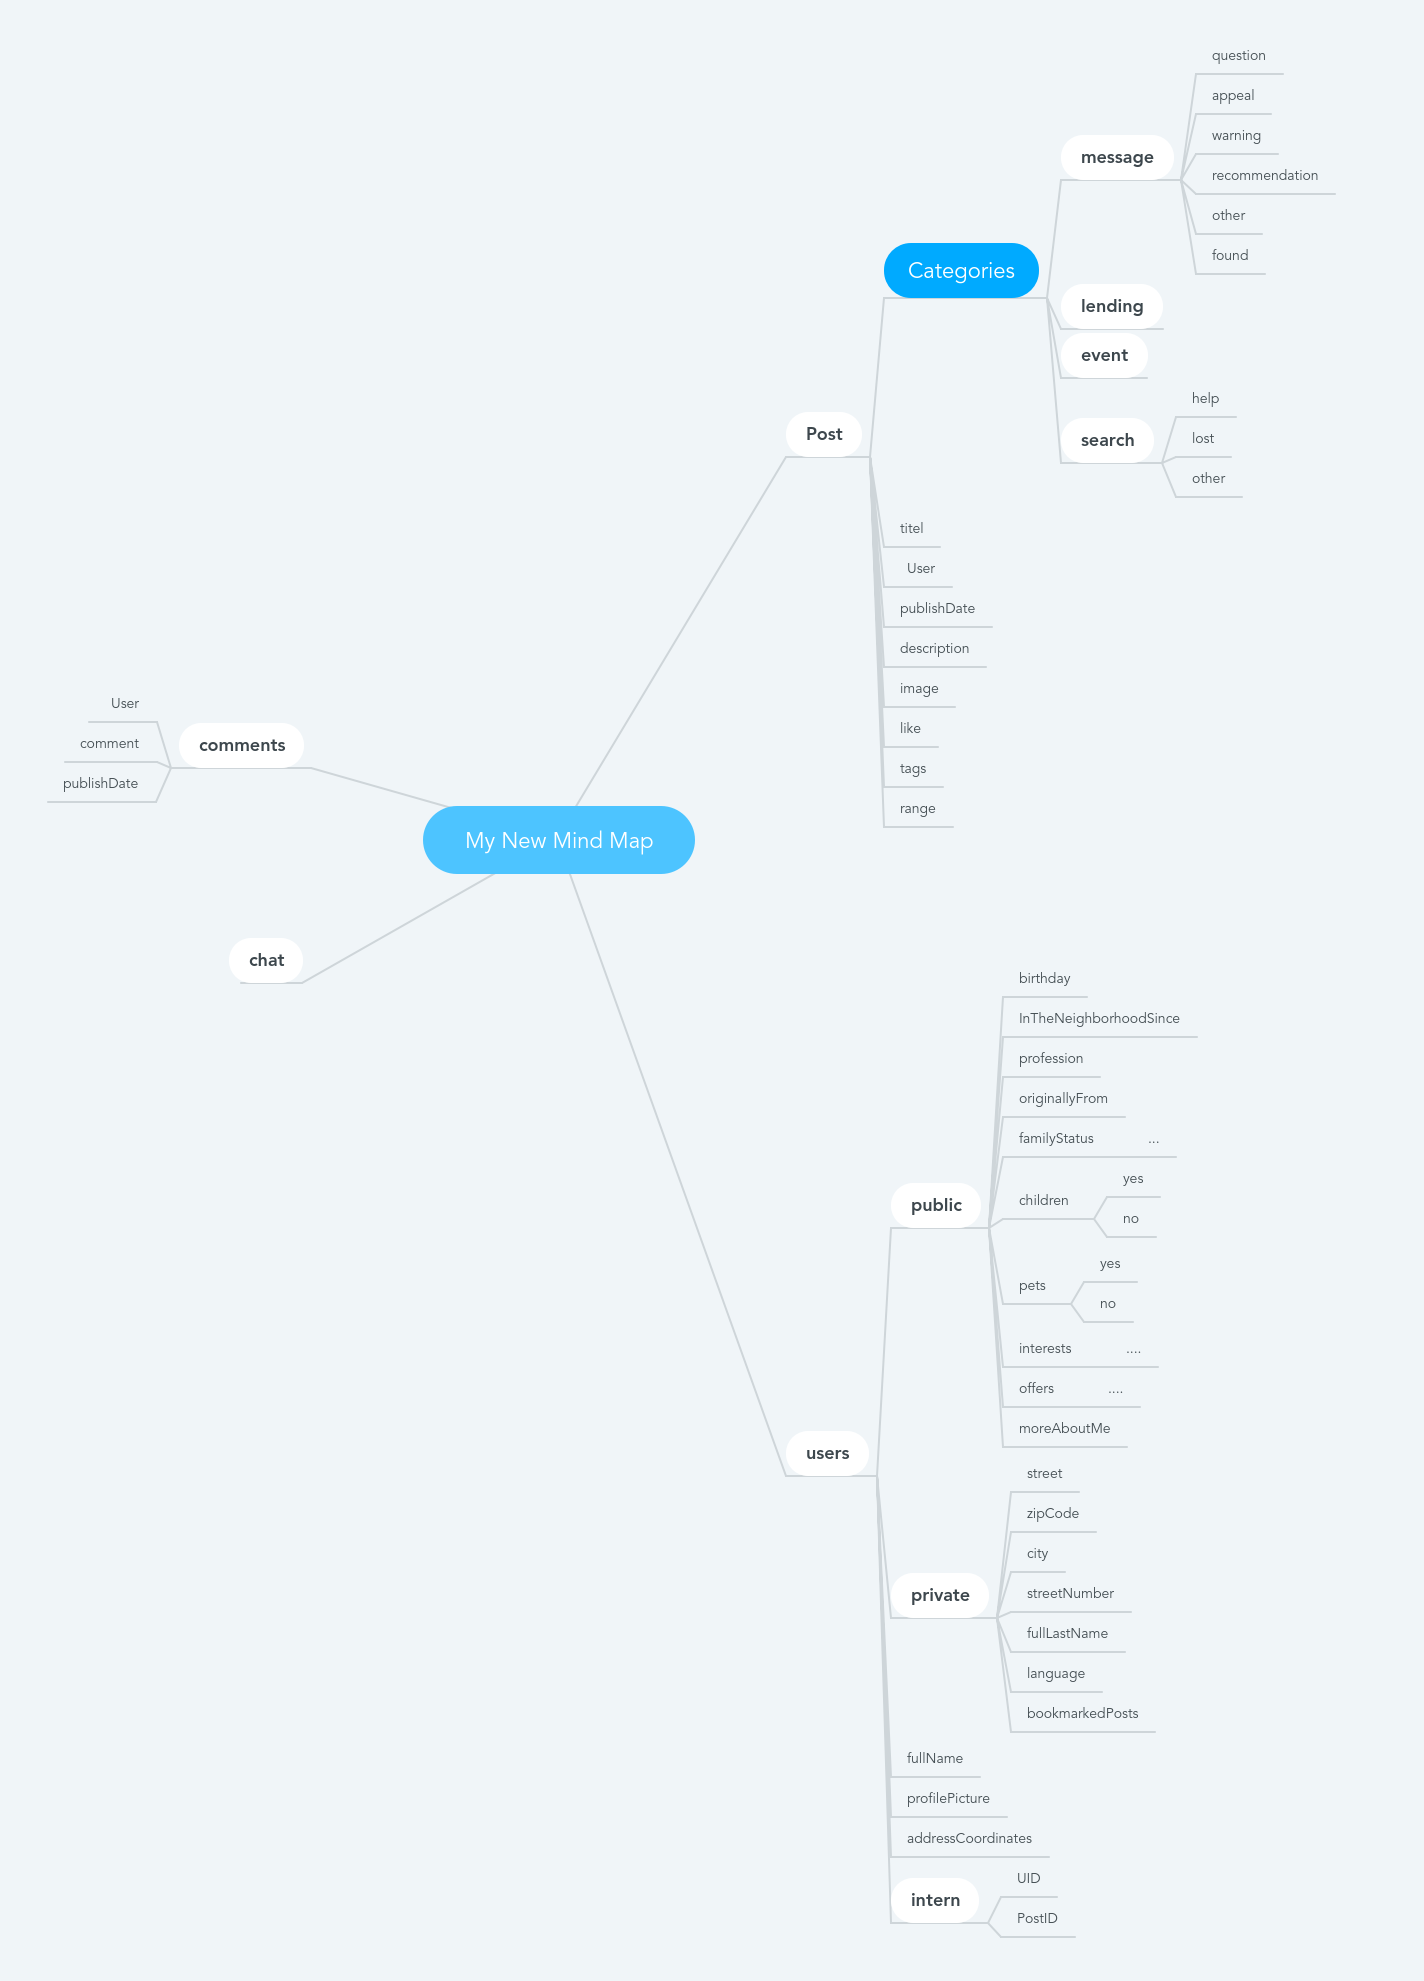
\includegraphics[width=0.8\textwidth]{pics/nochba-erd-old.png}
  \caption{Das erste Datenmodell}
  \label{fig:old-erd}
\end{figure}

Die vorliegende Grafik \ref{fig:old-erd} repräsentiert den Ansatz des ersten Datenmodells, welches im Zuge der Diplomarbeit erstellt wurde. Da das Team zum Zeitpunkt des Erstellens des Datenmodells über keine praktische Erfahrung mit Firestore oder mit NoSQL-Datenbanken verfügte, ist das Datenmodell dementsprechend unvollständig und lückenhaft.
\\\\
Es besteht aus vier Hauptsammlungen: \texttt{users}, \texttt{posts}, \texttt{comments} und \texttt{chats}
\\\\
\paragraph{Users}\mbox{} \\
Die \texttt{users}-Collection ist die Sammlung, die die Daten des Users aufbewahren sollte. Die Dokumente der Collection beinhalten die Felder \texttt{fullName} für den Anzeigename, \texttt{profilePicture} für das Profilbild und \texttt{addressCoordinates} für die Koordinaten des Users. Der Anzeigename ist der Name der den anderen Usern angezeigt wird und kann sich entweder aus dem Vor- und Nachnamen zusammensetzen (Max Mustermann) oder aus dem Vornamen und Initial des Nachnamen (Max M.). Weiters beinhaltet jedes Dokument die drei weiteren Sub-Collections \texttt{public}, \texttt{private} und \texttt{intern}.
\\\\
Die \texttt{public}-Collection beinhaltet öffentliche Informationen von dem User, die für jeden anderen User zugänglich sind. Die Dokumente der Collection beinhalten die folgenden Felder:
\begin{compactitem}
  \item \texttt{birthday} für den Geburtstag des Nachbarn oder der Nachbarin
  \item \texttt{InTheNeighbourhoodSince} für das Datum seitdem der Nachbar oder die Nachbarin in der Nachbarschaft ist
  \item \texttt{Profession} für den Beruf des Nachbarn oder der Nachbarin
  \item \texttt{originallyFrom} für den Heimatsort des Nachbarn oder der Nachbarin
  \item \texttt{familyStatus} für den Familienstatus des Nachbarn oder der Nachbarin
  \item \texttt{children} ob der Nachbar oder die Nachbarin Kinder hat
  \item \texttt{pets} ob der Nachbar oder die Nachbarin Haustiere hat
  \item \texttt{interests} für die Interessen des Nachbarn oder der Nachbarin
  \item \texttt{offers} für was angeboten werden kann von dem Nachbarn oder der Nachbarin
  \item \texttt{moreAboutMe} für eine genauere Selbst-Beschreibung des Nachbarn oder der Nachbarin
\end{compactitem}
Diese Daten werden vom User selbst festgelegt und dann beim öffentlichen Profil angezeigt.
\\\\
Die \texttt{private}-Collection beinhaltet private Informationen von dem User, zu denen kein anderer Zugriff hat. Daten die in diese Sammlung gespeichert werden, sind die Addresse mit Hilfe der Felder \texttt{street}, \texttt{streetNumber}, \texttt{city} und \texttt{zipCode}, der vollständige Nachname des Users mit dem Feld \texttt{fullLastName}, die eingestellte Sprache mit dem Feld \texttt{language} und die vom User durch Markierung gespeicherten Beiträge mit dem Feld \texttt{bookMarkedPosts}.
\\\\
Die \texttt{intern}-Collection beinhaltet interne Informationen von dem User, die für die saubere Funktionalität der App wichtig sind, wie die Benutzeridentifikationsnummer mit dem Feld \texttt{uid} und die geliketen Posts des Users mit dem Feld \texttt{postId}

\paragraph{Posts}\mbox{} \\
Die \texttt{posts}-Collection ist die Sammlung, die die Beiträge der User aufbewahren soll. Die Dokumente der Collection beinhalten die Felder \texttt{titel} für den Titel, \texttt{decription} für die Beschreibung, \texttt{image} für das anhängbare Bild, \texttt{tags} für die anhängbaren Tags, \texttt{range} für die Reichweite innerhalb der Beitrag nur gesehen werden soll, \texttt{like} für den Like-Zähler, \texttt{user} für die Benutzer-Id von dem der Beitrag stammt und \texttt{publishDate} für das Veröffentlichungsdatum. Als weiteres Feld zählt noch \texttt{category}, welches im DatenModell als eine Enumeration dargestellt wird.

\paragraph{Comments}\mbox{} \\
Die \texttt{comments}-Collection ist die Sammlung, die die Kommentare der Beiträge aufbewahren soll. Die Dokumente der Collection beinhalten die Felder \texttt{comment} für den Text, \texttt{user} für die Benutzer-Id von dem der Kommentar stammt und \texttt{publishDate} für das Veröffentlichungsdatum. In diesem Ansatz wurde auf die Id des Beitrags vergessen, unter welchem der Kommenater hinterlassen wurde.

\paragraph{Chats}\mbox{} \\
Obwohl die \texttt{chats}-Collection im ursprünglichen Datenmodell enthalten ist, sind die zugehörigen Felder und Strukturen nicht weiter definiert.

\begin{figure}[h]
  \centering
  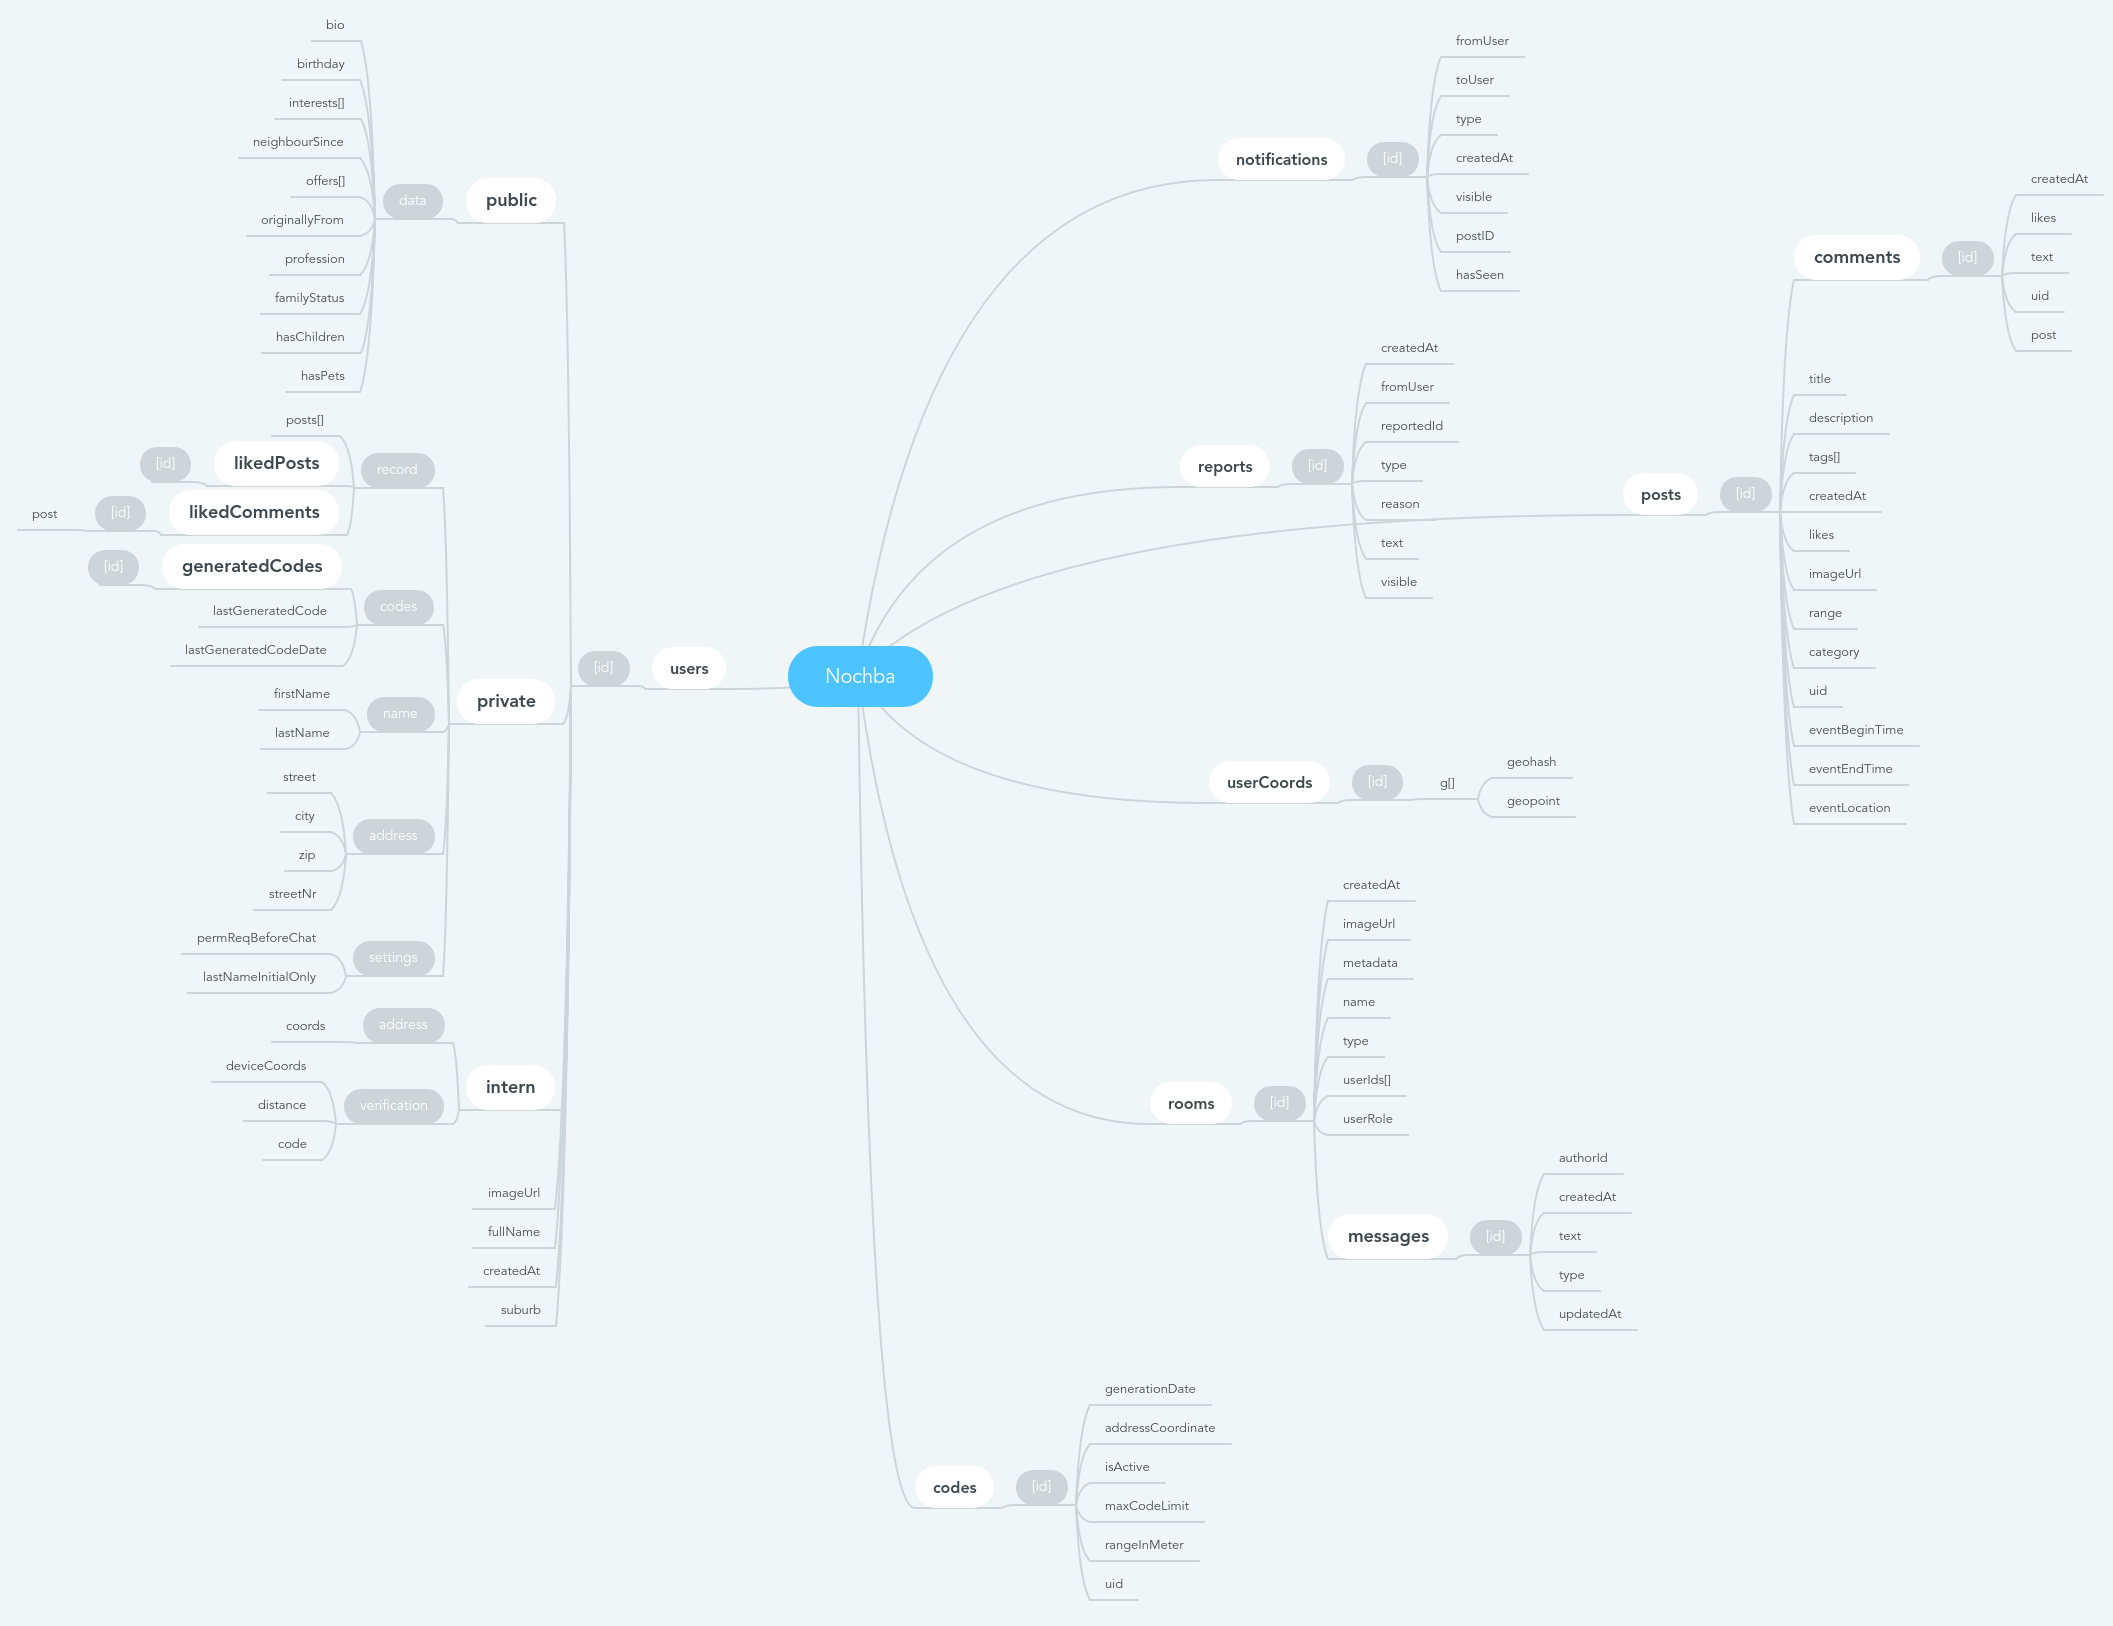
\includegraphics[width=1\textwidth]{pics/nochba-erd-new.png}
  \caption{Das neue Datenmodell}
  \label{fig:new-erd}
\end{figure}

Die vorliegende Grafik \ref{fig:new-erd} repräsentiert das aktuelle Datenmodell. Durch das erweitere Know-How, welches sich das Team im Lauf der Diplomarbeit angeeignet hat, wurde darauf geachtet eine möglichst effiziente Datenaufteilung und Datenspeicherung zu gestalten.
\\\\
Um das zu gewährleisten wurden folgende Prinzipien erstellt:
\begin{enumerate}
  \item Falls eine Collection abhängig von einer anderen Collection ist, wird diese der anderen Collection als Sub-Collection hinzugefügt - Beispiel: Beiträge und Kommentare
  \item Daten, die miteinander nichts zu tun haben werden in eigene Dokumente gespeichert
  \item Falls eine Collection einmalig verschiedene Daten speichern soll, so bekommen die Dokumente eine vorbstimmte Id, um das Verwalten der Dokumente zu erleichtern - Beispiel: Die \texttt{private}-Subcollection innerhalb der \texttt{users}-Collection beinhaltet das Dokument \texttt{name}, wo der Name gespeichert wird und das Dokument \texttt{address}, wo die Addressdaten gespeichert werden

\end{enumerate}

%\\\\
%Im Gegensatz zum alten Datenmodell wurde das neue Datenmodell um mehrere Collections erweitert und manche Collections wurden angepasst. Es besteht aus folgenden Hauptsammlungen: \texttt{users}, \texttt{posts}, \texttt{notifications}, \texttt{reports}, \texttt{codes} und \texttt{chats}
%\\\\

\paragraph{Users}\mbox{} \\
Die \texttt{users}-Collection ist die Sammlung, die die Daten des Users aufbewahren sollte. Die Dokumente der Collection beinhalten wie beim alten Datenmodell die Felder \texttt{fullName} für den Anzeigename und \texttt{profilePicture} für das Profilbild. Das Feld \texttt{addressCoordinates} für die Koordinaten des Users wurde entfernt, weil es sich als Datenleck von privaten Userdaten herausstellte. Die Felder der \texttt{users}-Collections dienen als Anzeigedaten, von daher wurde das \texttt{addressCoordinates}-Feld mit dem \texttt{suburb}-Feld ersetzt, was vielmehr das Stadtviertel oder die Gemeinschaft des Users speichern soll.
Der Ansatz, dass die \texttt{users}-Collection drei weitere Sub-Collections (\texttt{public}, \texttt{private} und \texttt{intern}) beinhalten soll wurde beibehalten.
\\\\
Die \texttt{public}-Collection beinhaltet öffentliche Informationen von dem User, die für jeden anderen User zugänglich sind. Die öffentlichen Daten werden unter dem Dokument \texttt{data} gspeichert. Die Datenfelder der öffentlichen Daten haben sich auf die Folgenden angepasst:
\begin{compactitem}
  \item \texttt{birthday} für den Geburtstag des Nachbarn oder der Nachbarin
  \item \texttt{InTheNeighbourhoodSince} für das Datum seitdem der Nachbar oder die Nachbarin in der Nachbarschaft ist
  \item \texttt{Profession} für den Beruf des Nachbarn oder der Nachbarin
  \item \texttt{originallyFrom} für den Heimatsort des Nachbarn oder der Nachbarin
  \item \texttt{interests} für die Interessen des Nachbarn oder der Nachbarin
  \item \texttt{offers} für was angeboten werden kann von dem Nachbarn oder der Nachbarin
  \item \texttt{bio} für eine genauere Selbst-Beschreibung des Nachbarn oder der Nachbarin
\end{compactitem}
Diese Daten werden nach wie vor vom User selbst festgelegt und dann beim öffentlichen Profil angezeigt. Der Grund für die Anpassungen ging dem Wunsch nach, das öffentliche Profil etwas simpler zu halten.
\\\\
Die \texttt{private}-Collection beinhaltet private Informationen von dem User, zu denen kein anderer Zugriff hat. Zur besseren Aufteilung wurden die privaten Daten des Users auf mehrere Dokumente aufgeteilt.
\\
Das Dokument \texttt{name} beinhaltet den Vornamen und Nachnamen, was ---.
\\
Als nächstes ist das Dokument \texttt{address}, welches die Addressdaten des Users beinhaltet, also das Feld \texttt{street} für die Straße, das Feld \texttt{streetNumber} für die Straßennummer, das Feld \texttt{city} für die Stadt und das Feld \texttt{zip} für die Postleitzahl.
\\
Ein für den Nutzungswert der App wichtiges Dokument ist das Dokument \texttt{records}, welches die vom User markierten und geliketen Beiträge speichern soll. Das Dokument beinhaltet das Feld \texttt{posts}, welches die vom User markierten Posts speichert. Das Dokument beinhaltet außerdem zwei Sub-Collections: \texttt{likedPosts} und \texttt{likedComments}. Diese zwei Subcollections speichern die vom User geliketen Beiträge bzw. Kommentare. Die Funktionsweise der Subcollection \texttt{likedPosts} baut auf dem Konzept auf, dass die angelegten Entitäten nach der Id des Beitrags erstellt werden. Das heißt, dass die angelegte Entität die gleiche Id hat, wie der Beitrag, welcher vom User markiert wurde und sonst nichts. Das soll für eine möglichst effiziente Datenspeicherung sorgen. Die Funktionsweise der Subcollection \texttt{likedComments} baut auf dem selben Konzept auf, nur mit der Id des Kommentars als Entitäts-Id und zusätzlich wird noch die Id des Beitrags unter dem der Kommentar gelassen wurde mitgespeichert.
\\
Das nächste Dokument \texttt{settings} soll die Benutzereinstellungen speichern. Darunter zählt das Feld \texttt{lastNameInitialOnly}, mit welchem der User bestimmt, ob sein ganzer Name angezeigt werden soll oder nur der Vorname mit dem Initial des Nachnamens, und \texttt{permReqBeforeChat}, mit welchem der User bestimmt, ob er/sie eine Anfrage erhalten möchte, bevor er/sie angeschrieben wird.
\\
Das letzte Dokument \texttt{codes} soll die vom User erstellten Einlade-QR-Codes speichern. Um alle Einlade-QR-Codes vom User mittracken zu können, werden alle QR-Codes in einer Subcollection \texttt{generatedCodes} gesammelt. Der zuletzt generierte QR-Code und das Datum der Erstellung werden in die Felder \texttt{lastGeneratedCode} und \texttt{lastGeneratedCodeDate} gespeichtert.
\\\\
Die \texttt{intern}-Collection beinhaltet interne Informationen von dem User, die für die saubere Funktionalität der App wichtig sind. In dem neuen Datenmodell beinhaltet das Dokument zwei Dokemente: \texttt{address} und \texttt{verification}.
\\
Im Dokument \texttt{address} werden im Feld \texttt{coords} die Koordinaten der angegeben Addresse gespeichert.
\\
Falls sich der User durch einen Einlade-QR-Code verifiziert hat, hat das Dokument \texttt{verification} die Felder \texttt{deviceCoords} für die Gerätkoordinaten, \texttt{code} für den Einlade-QR-Code der eingesetzt wurde und \texttt{distance}, welches angibt wie groß die Distanz zwischen den Gerätkoordinaten und den Koordinaten des QR-Codes ist.

\paragraph{Codes}\mbox{} \\
Die \texttt{codes}-Collection ist die Sammlung, wo alle QR-Codes die jemals erzeugt wurden, gespeichert ist. Die Dokumente der Collection beinhalten die Felder \texttt{coords} und \texttt{range} für die Koordinaten und Reichweite innerhalb der QR-Code gültig ist, \texttt{isActive} ob der Code noch gültig ist, \texttt{createdAt} für das Veröffentlichungsdatum, \texttt{maxCodeLimit} für wie viele User mit diesem Einlade-QR-Code eingeladen werden können und \texttt{uid} für den User der den QR-Code erzeugt hat.

\paragraph{Posts}\mbox{} \\
Die \texttt{posts}-Collection ist die Sammlung, die die Beiträge der User aufbewahren soll. Die Felder der Dokumente der Collection haben sich im Vergleich zum alten Datenmodell nicht verändert.
\\
Was sich im Datenmodell im Bezug auf die Beiträge verändert hat, ist dass die \texttt{comments}-Collection als Subcollection zur \texttt{posts}-Collection hinzugefügt wurde. Die Felder der Dokumente der \texttt{comments}-Collection haben sich auch angepasst. Die Dokumente der Collection beinhalten die Felder \texttt{text} für den Text, \texttt{likes} für den Like-Zähler, \texttt{createdAt} für das Veröffentlichungsdatum, \texttt{uid} für die Id des Users, welcher den Kommentar hinterlassen hat, und \texttt{postId} für die Id des Beitrags unter welchem der Kommentar hinterlassen wurde.

\paragraph{Notifications}\mbox{} \\
Die \texttt{notification}-Collection ist die Sammlung, die die Benachrichtigungen der User aufbewahren soll. Benachrichtigungen sollen den User über neue Chat-Anfragen benachrichtigen. Die Dokumente der Collection beinhalten die Felder \texttt{fromUid} und \texttt{toUID} für den User der die Benachrichtigung abgeschickt hat und den User der die Benachrichtigung erhält, \texttt{createdAt} für das Erstellungsdatum, \texttt{visible} ob die Benachrichtigung für den User sichtbar ist, \texttt{hasSeen} ob der User die Benachrichtigung gesehen hat und falls die Chat-Anfrage von einem Beitrag kommt noch das Feld \texttt{postId} für die Id des Beitrags. Außerdem existiert noch das Feld \texttt{type}, die den Typ der Anfrage beschreiben soll. Es gibt zwei Typen. Ein \texttt{postRequest} um für das Antworten eines Beitrags eine Chat-Anfrage zu erstellen und ein \texttt{userRequest} um zum Kontakt erstellen zu einen User eine Chat-Anfrage zu erstellen.

\paragraph{Reports}\mbox{} \\
Die \texttt{reports}-Collection ist die Sammlung, wo die Meldungen auf Beiträge oder User gespeichert werden. Die Dokumente der Collection beinhalten die Felder \texttt{fromUser} für den User der die Meldung abgeschickt hat, \texttt{text} für die Erklärung warum die Meldung abgeschickt wurde, \texttt{createdAt} für das Erstellungsdatum, \texttt{visible} ob die Meldung für den User sichtbar ist und \texttt{reason} für den ausgewählten Grund warum die Meldung abgeschickt wurde. Außerdem existiert noch das Feld \texttt{type}, welches angibt, was gemeldet wurde. Es kann entweder ein Beitrag, Kommentar oder User gemeldet werden. Daneben gibt es noch das Feld \texttt{reportedId}, was die Id vom jeweiligen Beitrag, Kommentar oder User speichert.

\paragraph{Chats}\mbox{} \\
Die \texttt{chats}-Collection ist die Sammlung, wo die Chats und dazugehörigen Nachrichten der User gespeichert werden.


\subsection{Cloud Storage}
\setauthor{Sandin Habibovic}
Der Cloud Storage fungiert in der Applikation als Speicherlösung für Bilder, einschließlich Profilbilder und Bilder, die zu Beiträgen hinzugefügt werden.

\subsubsection{Aufbau}
\setauthor{Sandin Habibovic}
\begin{itemize}
  \item profile
        \begin{itemize}
          \item pictures
        \end{itemize}
  \item posts
        \begin{itemize}
          \item {uid}
                \begin{itemize}
                  \item pictures
                \end{itemize}
        \end{itemize}
\end{itemize}

Die Dateistruktur teilt sich in zwei Ordner auf: \texttt{profile} und \texttt{posts}.
\\\\
Im Ordner \texttt{profile} werden die Profilbilder der User gesichert. Dabei werden die Namen der Profilbilder als Id der User gesetzt, um das effizientere Speichern und Suchen von Profilbilder einzelner User zu erreichen.
\\\\
Im Ordner \texttt{posts} werden die Bilder die zu Beiträge gehören gesichert. Dabei besitzt der \texttt{posts}-Ordner noch weitere Unterordner die nach der Id der User benannt werden. Das soll garantieren, dass die Bilder, die von User hochgeladen werden, nur in deren Ordner gespeichert werden.

\subsubsection{Funktionsweise}
\setauthor{Sandin Habibovic}

\begin{lstlisting}[caption=uploadProfileImageToStorage Funktion,label=lst:uploadProfileImageFunction]
  Future<String> uploadProfileImageToStorage(Uint8List file) async {
    final authService = Get.find<AuthService>();

    final uid = authService.uid;

    if (uid.isEmpty) {
      return '';
    }

    Reference ref = FirebaseStorage.instance.ref().child('profile/$uid');
    UploadTask uploadTask = ref.putData(file);

    TaskSnapshot snap = await uploadTask;
    String downloadUrl = await snap.ref.getDownloadURL();
    return downloadUrl;
  }

\end{lstlisting}
Der vorliegende Code \ref{lst:uploadProfileImageFunction} soll die Funktionsweise des Cloud Storage demonstrieren. Die Funktion soll das Profilbild des Users im Cloud Storage einspeichern. Im Code lässt sich sehen, dass die Funktion das Bild in Form einer \texttt{Uint8List} bekommt und sich zuerst die Id des aktuellen Users durch den \texttt{AuthService} holt. Danach wird eine Referenz zum Cloud Storage auf den Pfad \texttt{profile/\$uid} gebildet und die Bilddatei wird auf die Referenz hochgeladen. Wenn das Hochladen erfolgreich war, wird die URL, unter der das Bild verfügbar ist, zurüchgegeben. Diese URL kann dann in den Userdaten unter der \texttt{users}-Collection im Feld \texttt{imageUrl} gespeichert werden.

\subsection{Firebase Cloud Functions}
\setauthor{Martin Hausleitner}
Firebase Cloud Functions sind eine großartige Möglichkeit,
um Business-Logik abzubilden. Es handelt sich um serverlose
Funktionen, die in JavaScript oder TypeScript geschrieben
werden und einzeln auf der Google Cloud gehostet werden. Je
nach Nachfrage werden sie automatisch skaliert oder komplett
abgeschaltet. Ein Nachteil ist, dass die Startup-Zeit länger
sein kann als bei einem herkömmlichen Backend, das immer
läuft. Allerdings kann man durch Cloud Functions viel Geld
sparen, da nur die Prozessorlaufzeit bezahlt werden muss.

Firebase Cloud Functions ermöglichen es Entwicklern, auf verschiedene Ereignisse in Firebase-Produkten zu reagieren. Zum Beispiel, wenn sich Daten in der Firestore-Datenbank ändern oder ein neuer Nutzer in Firebase Authentication registriert wird. Wenn ein solches Ereignis eintritt, wird die entsprechende Cloud Function automatisch ausgeführt.

Alle Cloud Functions wurden in TypeScript entwickelt, da diese Programmiersprache Typsicherheit und verbesserte Fehlererkennung bietet.

\subsubsection{Überprüfen der Addresse}
\setauthor{Sandin Habibovic}

Die Cloud-Funktion \texttt{checkAddress} erfordert eine authentifizierte Anfrage und erhält eine Adresse vom User, die aus Straße, Hausnummer, Stadt und Postleitzahl besteht.
\\
Um sicherzustellen, dass die Anfrage authentifiziert ist, wird zuerst überprüft, ob der Aufrufer authentifiziert ist. Wenn das nicht der Fall sein sollte, wird eine Fehlermeldung ausgegeben, die besagt, dass die Anfrage nicht authentifiziert ist.
\\
Die Funktion überprüft danach, ob alle erforderlichen Daten für die Adresse vorhanden sind. Wenn Daten fehlen, wird eine Fehlermeldung ausgegeben, die besagt, dass gültige Adressdaten benötigt werden.
\\
Die Adresse wird dann formatiert und an die Funktion \texttt{getOSMCoordinatesFromAddress} übergeben, um die Koordinaten der Adresse abzurufen. Wenn ein Fehler auftritt, was passieren kann, wenn eine nicht existierende Addresse angegeben wird, wird eine Fehlermeldung ausgegeben, die besagt, dass die Koordinaten nicht abgerufen werden konnten.
\\
Falls die Addresse verifiziert werden konnte, werden die Addressdaten vom User, also Straße, Hausnummer, Stadt und Postleitzahl, im Firestore gespeichert.
\\
Am Ende gibt die Funktion \texttt{true} zurück, um anzuzeigen, dass die Verifizierung erfolgreich abgeschlossen wurde.

\subsubsection{Registrierung mit einem Verifizierungscode}\label{subsec:registrierung-verify}
\setauthor{Martin Hausleitner}

Die Cloud-Funktion \texttt{checkVerificationCode} wird ausgeführt, wenn ein Nutzer sich mit einem Verifizierungscode registrieren möchte. Wenn der Benutzer nicht authentifiziert ist, wird eine \texttt{HttpsError} ausgelöst. Dann wird der Verifizierungscode überprüft, um sicherzustellen, dass er die korrekte Formatierung hat. Wenn der Code ungültig ist, wird eine weitere \texttt{HttpsError} ausgelöst.

Als Nächstes wird der Verifizierungscode mit der Datenbank abgeglichen, um sicherzustellen, dass er aktiv und noch nicht zu oft verwendet wurde. Wenn der Code erfolgreich validiert wird, wird die Adresse des Benutzers abgerufen und deren Koordinaten mithilfe einer API call an OpenStreetMap mit der Funktion \texttt{getOSMCoordinatesFromAddress} ermittelt. Dann wird die Entfernung zwischen der Adresse des Benutzers und der Adresse, die dem Verifizierungscode zugeordnet ist, berechnet mit der Funktion \texttt{getDistanceFromLatLonInMeters}. Wenn die Entfernung nicht innerhalb des zulässigen Bereichs liegt, wird eine weitere \texttt{HttpsError} ausgelöst.

Schließlich werden die Informationen des Benutzers und des Verifizierungscodes in der Datenbank aktualisiert, um anzuzeigen, dass der Benutzer erfolgreich verifiziert wurde. Die Cloud-Funktion gibt \texttt{true} zurück, um anzuzeigen, dass die Verifizierung erfolgreich war.

In jeder Phase der Funktion wird ein Logger verwendet, um Informationen über den Status der Funktion zu protokollieren.

\subsubsection{Regestrierung mit Gerät Koordinaten}
\setauthor{Martin Hausleitner}

Die Cloud-Funktion \texttt{checkAddressWithDeviceLocation} erfordert eine authentifizierte Anfrage und erhält eine Adresse sowie Längen- und Breitengradkoordinaten vom Gerät des Benutzers. Die Funktion prüft, ob alle erforderlichen Daten vorhanden sind und ruft dann die Funktion \texttt{getOSMCoordinatesFromAddress} auf, um die Koordinaten der angegebenen Adresse zu erhalten. Es wird auch die Funktion \texttt{getDistanceFromLatLonInMeters} aufgerufen, um die Entfernung zwischen der Adresse und den Koordinaten des Geräts des Benutzers zu berechnen.

Wenn die Entfernung größer ist als ein vordefinierter maximaler Abstand, wird eine Fehlermeldung ausgegeben und die Funktion gibt \texttt{false} zurück. Andernfalls speichert die Funktion die Koordinaten der Adresse und die Entfernung zwischen den Koordinaten des Geräts des Benutzers und der Adresse in der Firestore-Datenbank. Die Funktion ruft auch die Funktion \texttt{getOSMSuburbFromCoords} auf, um den Vorort der Adresse zu erhalten, und speichert diesen ebenfalls in der Firestore-Datenbank.

Die Funktion gibt \texttt{true} zurück, wenn die Verifizierung erfolgreich abgeschlossen ist.

In jeder Phase der Funktion wird ein Logger verwendet, um Informationen über den Status der Funktion zu protokollieren.

\subsubsection{Verifizierungscode generieren}
\setauthor{Martin Hausleitner}
Die Cloud-Funktion \texttt{generateVerificationCode} definiert Konstanten für das Intervall zwischen der Generierung von Codes, die maximale Anzahl von Codes und die Reichweite in Metern.

Anschließend wird der letzte Code des Nutzers aus der Datenbank geholt, um zu überprüfen, ob seit dem letzten generierten Code ausreichend Zeit vergangen ist. Wenn ja, wird der zuletzt generierte Code zurückgegeben.

Wenn nicht, wird eine Schleife gestartet, um einen neuen Code zu generieren mit der Funktion \texttt{generateRandomVerificationCode}. Der generierte Code wird dann mit Firestore abgeglichen, um sicherzustellen, dass er nicht bereits verwendet wurde.

Wenn der generierte Code eindeutig ist, wird überprüft, ob der Benutzer verifiziert ist. Wenn dies nicht der Fall ist, wird ein Fehler zurückgegeben. Andernfalls wird der generierte Code in die Firestore-Datenbank eingefügt, um den letzten generierten Code und das Datum der Generierung zu speichern.

Das Skript gibt dann den generierten Code zurück. In jeder Phase der Funktion wird ein Logger verwendet, um Informationen über den Status der Funktion zu protokollieren.

\subsubsection{Koordienaten von einer Adresse bestimmen}
\setauthor{Martin Hausleitner}
Für die Verifizierung ist es von Bedeutung, die Adresse des Nutzers in Koordinaten umzuwandeln, um im Backend damit arbeiten zu können. Ursprünglich wurde die Google Geocode API verwendet, jedoch ist diese kostenpflichtig. Eine passendere Alternative, die besser zur Projektphilosophie passt, wurde gefunden: Nominatim. Nominatim ist eine Open-Source-Geocoding-API für OpenStreetMap-Daten und bietet eine kostenlose API für diese spezielle Anforderung.

Die Funktion \texttt{getOSMCoordinatesFromAddress} nutzt die Bibliothek \texttt{axios}, um eine Anfrage an die Nominatim-API zu senden. Die API wird genutzt, um Koordinaten für eine Adresse zu erhalten.

Die Funktion nimmt einen Parameter \texttt{address} vom Typ \texttt{string} entgegen, welcher die Adresse enthält, für die Koordinaten abgerufen werden sollen.

Mithilfe von \texttt{axios.get} wird eine HTTP GET-Anfrage an die Nominatim-API gesendet. Die Adresse wird als URL-Parameter im Format \texttt{q=Adresse} übergeben. Die API liefert die Koordinaten als JSON-Objekt zurück, welches in der Variable \texttt{data} gespeichert wird.

Die Funktion überprüft dann, ob die Anfrage ein Ergebnis zurückgeliefert hat. Falls nicht, wird eine Fehlermeldung mit der Adresse ausgegeben.

Wenn ein Ergebnis vorhanden ist, wird das erste Ergebnis (in der Variable \texttt{firstResult}) verwendet, um eine neue Instanz der \texttt{GeoPoint}-Klasse zu erstellen. Diese Klasse ist Teil der Firebase-Admin-Bibliothek und ermöglicht die Speicherung von geografischen Koordinaten in einer Firestore-Datenbank.

\subsubsection{Entferung von zwei Nutzern berechnen}
\setauthor{Martin Hausleitner}
Die Cloud-Funktion \texttt{getDistanceFromTwoUsers} berechnet die Entfernung zwischen zwei Benutzern. Die Funktion erwartet eine \texttt{PostId} und einen authentifizierten Benutzer. Dann wird eine Überprüfung durchgeführt, ob der Post mit der angegebenen ID existiert und ob der Post eine gültige Reichweite hat. Es werden auch Überprüfungen durchgeführt, ob die Benutzerkoordinaten vorhanden sind, und ob die Entfernung zwischen beiden Benutzern innerhalb des Postbereichs liegt.

Die Funktion nutzt die importierten Funktionen \texttt{getDistanceFromLatLonInMeters} und \texttt{getNearestDistance}, um die Entfernung in Metern zu berechnen. Allerdings wird die berechnete Distanz grob gerundet, um die Privatsphäre der Nutzer zu wahren. Dabei werden die Längen- und Breitengradkoordinaten von zwei Benutzern miteinander verglichen, die aus der Firestore-Datenbank abgerufen werden. Wenn die Entfernung größer als die Reichweite des Posts ist, wird ein Fehler ausgegeben.

Schließlich gibt die Funktion die Entfernung zurück.

\subsubsection{Entfernung von zwei geographischen Koordinaten berechnen}
\setauthor{Martin Hausleitner}

\begin{lstlisting}[language=Java,caption=getDistanceFromLatLonInMeters Funktion,label=lst:getDistanceFunction]
    export function getDistanceFromLatLonInMeters(
        lat1: number,
        lon1: number,
        lat2: number,
        lon2: number
      ) {
        if (lat1 < -90 || lat1 > 90 || lon1 < -180 || lon1 > 180) {
          throw new Error(
            "Invalid coordinate: lat1 must be between -90 and 90, lon1 must be between -180 and 180"
          );
        }
        if (lat2 < -90 || lat2 > 90 || lon2 < -180 || lon2 > 180) {
          throw new Error(
            "Invalid coordinate: lat2 must be between -90 and 90, lon2 must be between -180 and 180"
          );
        }
        const R = 6371; // Radius der Erde in km
        const dLat = deg2rad(lat2 - lat1); // deg2rad unten
        const dLon = deg2rad(lon2 - lon1);
        const a =
          Math.sin(dLat / 2) * Math.sin(dLat / 2) +
          Math.cos(deg2rad(lat1)) *
            Math.cos(deg2rad(lat2)) *
            Math.sin(dLon / 2) *
            Math.sin(dLon / 2);
        const c = 2 * Math.atan2(Math.sqrt(a), Math.sqrt(1 - a));
        const d = R * c * 1000; // Distanz in Metern
      
        if (lat1 === lat2 && lon1 === lon2) return 0;
        return d;
      }
      
      function deg2rad(deg: number) {
        return deg * (Math.PI / 180);
      }
      
\end{lstlisting}
Der vorliegende Code \ref{lst:getDistanceFunction}
implementiert eine Funktion, die die
Distanz in Metern zwischen zwei geographischen Koordinaten
(Breitengrad und Längengrad) auf der Erdoberfläche
berechnet. Die Funktion nutzt die Haversine-Formel, welche auf Kugelgeometrie basiert und aus der Quelle \cite{movabletype} movabletype in Javascript übernommen wurde, um die kürzeste Entfernung zwischen zwei Punkten auf der Erdoberfläche zu berechnen.

Die Funktion \texttt{getDistanceFromLatLonInMeters} hat vier Parameter: \texttt{lat1} und \texttt{lon1} sind die Breiten- und Längengrade des ersten Punktes, während \texttt{lat2} und \texttt{lon2} die Breiten- und Längengrade des zweiten Punktes sind, zwischen denen die Distanz berechnet werden soll.

Zu Beginn des Codes werden die Eingabeparameter auf ihre Gültigkeit geprüft und eine Fehlermeldung wird ausgegeben, falls eine der Koordinaten außerhalb des Bereichs von \texttt{-90} bis \texttt{90} für die Breite und \texttt{-180} bis \texttt{180} für die Länge liegt.

Die Funktion berechnet dann die Differenzen der Breiten- und Längengrade sowie den Radius der Erde (\texttt{R}) in Kilometern. Die Differenzen werden dann in Radianten umgewandelt und die Haversine-Formel wird angewendet, um die Entfernung in Kilometern zu berechnen. Schließlich wird das Ergebnis in Meter umgewandelt und zurückgegeben.

Die Funktion \texttt{deg2rad} wird als Hilfsfunktion definiert, um Grad in Radianten umzurechnen.

Die Funktion gibt \texttt{0} zurück, falls die beiden Eingabeparameter denselben Wert haben, um zu vermeiden, dass eine sehr kleine Distanz als Ergebnis ausgegeben wird, wenn es sich um denselben Punkt handelt.


\subsubsection{Bestimmung der nächstgelegenen Entfernung}
\setauthor{Martin Hausleitner}
Zur Wahrung der Privatsphäre der Nachbarn ist eine Funktion erforderlich, die den nächstgelegenen Abstand zu den Nachbarn angibt, ohne den genauen Abstand offenzulegen. Diese Funktion trägt den Namen \texttt{getNearestDistance} und erhält einen Meterwert als Parameter.

Die Funktion erstellt ein Array mit den Optionen \texttt{[100, 200, 500, 1000, 5000, 10000, 15000]} und setzt die Variable \texttt{nearest} auf den ersten Wert im Array.

Dann wird eine Schleife ausgeführt, die durch jedes Element im Array \texttt{options} geht und prüft, welches Element am nächsten zum angegebenen Abstand \texttt{distance} liegt. Wenn ein Element näher ist als das bisher am nächsten liegende Element, wird \texttt{nearest} aktualisiert.

Letztendlich wird geprüft, ob \texttt{nearest} größer oder gleich 1000 ist. Abhängig davon wird der Abstand entweder in Kilometern oder Metern zurückgegeben. Ist der Abstand größer oder gleich 1000, wird die Einheit \texttt{km} hinzugefügt, andernfalls wird \texttt{m} verwendet. Verzichtet wurde bewusst auf Switches oder If-Bedingungen, da mit der aktuellen Funktion schneller Abstände geändert werden können. Die Evaluierung des Arrays mit den Optionen ist noch im Gange.


\subsubsection{Nachbarschaft von Nutzer bestimmen}
\setauthor{Martin Hausleitner}
Um den App-Nutzern ein besseres Verständnis der Nachbarschaften zu vermitteln, in denen ihre Nachbarn leben, wird bei jedem Benutzer die jeweilige Nachbarschaft angezeigt. Diese Information wird automatisch in der Datenbank gespeichert, sobald der Nutzer verifiziert ist. Zur Umsetzung dieser Funktion wird eine Methode eingesetzt, die die geografischen Koordinaten des Benutzers verwendet, um die entsprechende Nachbarschaft mithilfe der OpenStreetMap-API abzurufen:

Die Funktion heißt \texttt{getOSMSuburbFromCoords} und nimmt zwei Parameter entgegen: \texttt{lat} für die geografische Breite und \texttt{lon} für die geografische Länge des Benutzers. Diese Funktion gibt eine Promise zurück, die eine Zeichenfolge \texttt{String} mit dem Namen der Nachbarschaft des Benutzers enthält. Die Funktion verwendet die Axios-Bibliothek, um eine GET-Anfrage an die OpenStreetMap-API zu senden. Diese Anfrage enthält die geografischen Koordinaten des Benutzers und die gewünschte Zoomstufe \texttt{18}, um die Nachbarschaft zu finden. Wenn die Anfrage erfolgreich ist, gibt die Funktion den Namen der Nachbarschaft zurück, der aus den Daten extrahiert wird, die von der API zurückgegeben werden. Wenn der Name der Nachbarschaft nicht verfügbar ist, gibt die Funktion den Namen der Stadt oder der Gemeinde zurück, in der sich der Benutzer befindet. Wenn auch diese Informationen nicht verfügbar sind, gibt die Funktion \texttt{null} zurück. Wenn bei der Anfrage ein Fehler auftritt, wird eine Fehlermeldung ausgelöst.


\subsubsection{Beiträge von Nachbarn in der Umgebung ermitteln}
\setauthor{Sandin Habibovic}

Die Cloud Function \texttt{getUserPostsWithinRange} ist dafür verantwortlich, Beiträge von User innerhalb einer bestimmten Reichweite abzurufen. Dies wird durch den Aufruf von Firestore und GeoFireStore erreicht, um die User innerhalb des Bereichs zu ermitteln und dann ihre Beiträge abzurufen.
\\
GeoFirestore ist eine Open-Source-Bibliothek, die auf der Firebase-Plattform basiert und die Funktionen von Firestore erweitert, um Geofencing und so die Filterung von Daten nach geografischen Entfernungen und Koordinaten zu ermöglichen.
Quelle: https://geofirestore.com
\\
Die Cloud Function bekommt als Parameter die Rechweite innerhalb der gefiltert werden soll und prüft zunächst, ob der User authentifiziert ist. Wenn nicht, wird ein Fehler ausgelöst, der besagt, dass die Anfrage nicht authentifiziert ist. Wenn der User authentifiziert ist, wird seine Id verwendet, um seine Koordinaten aus der Firestore-Datenbank abzurufen.
\\
Die Funktion verwendet dann GeoFireStore, um alle User innerhalb der mitgegebenen Reichweite zu ermitteln mit den Userkoordinaten als Mittelpunkt. Diese emittelten User werden dann gefiltert, um deren Beiträge aus der Firestore-Datenbank abzurufen.
\\
Um sicherzustellen, dass der User innerhalb der Reichweite in der, der Beitrag sichtbar sein soll, liegt, wird für jeden Beitrag die Entfernung zwischen dem User, der die Cloud Functions aufgerufen hat, und dem User, der den Beitrag erstellt hat, berechnet. Wenn die Entfernung kleiner als die Reichweite innerhalb der Beitrag sichtbar sein soll ist, wird der Beitrag in die Liste der gültigen Beiträge aufgenommen.
\\
Schließlich gibt die Funktion eine Liste mit den Ids der gültigen Beiträge zurück, die innerhalb der mitgegebenen Reichweite liegen.
\\
Die vorliegende Grafik \ref{fig:near-neighbours} zeigt die Funktionsweise der Cloud Function beispielsweise als Bild an.

\begin{figure}[h]
  \centering
  \includegraphics[width=1\textwidth]{pics/nachbarn-in-der-nähe.JPG}
  \caption{Reichweiten verschiedener Nachbarn}
  \label{fig:near-neighbours}
\end{figure}

\subsubsection{Verifizierungscode format überprüfen}
\setauthor{Martin Hausleitner}
Um die Laufzeit bei der Verifizierung von Cloud-Funktionen zu optimieren, ist es sinnvoll, am Anfang der Verifizierung eine Überprüfung durchzuführen, ob der Verifizierungscode das richtige Format hat. Dazu wird die Funktion \texttt{verifyVerificationCode} genutzt werden, welche einen \texttt{String} als Parameter erwartet und einen \texttt{Boolean}-Wert zurückgibt. In der Funktion wird ein regulärer Ausdruck Regex definiert, um sicherzustellen, dass der Verifizierungscode den Anforderungen entspricht. Der Regex lautet \texttt{/}\verb|^[a-zA-Z0-9]{10}$/|\texttt{,} was bedeutet, dass der Code aus genau 10 alphanumerischen Zeichen bestehen muss. Mit der Methode \texttt{checkVerificationCode} wird der übergebene Code auf Übereinstimmung mit dem Regex geprüft und das Ergebnis als \texttt{Boolean}-Wert zurückgegeben.

\subsubsection{Verifizierungscode generator}
\setauthor{Martin Hausleitner}

Die Funktion \texttt{generateRandomVerificationCode} erzeugt einen zufälligen Code mit einer Länge von 10 Zeichen, indem sie eine Kombination aus Groß- und Kleinbuchstaben des englischen Alphabets sowie Ziffern von 0 bis 9 verwendet. Dabei wird \texttt{Math.random()} zur Generierung einer Zufallszahl zwischen 0 und 1 genutzt und mit der Länge des Zeichenfolgen-Arrays multipliziert, um eine zufällige Position innerhalb des Arrays auszuwählen. Anschließend wird das ausgewählte Zeichen an das Ergebnis angehängt und dieser Schritt wird für jedes Zeichen wiederholt, bis eine Zeichenkette der Länge 10 generiert wurde.

Diese Funktion wird in der Cloud-Funktion \texttt{generateVerificationCode} verwendet, um einen zufälligen Code zu generieren. Es ist wichtig, dass der Code-Generator in der Lage ist, eine ausreichende Anzahl von Codes zu generieren, damit es keine Kollisionen gibt. Da jeder Code zufällig generiert wird und die Funktion eine zufällige Zeichenkette aus 62 möglichen Zeichen erzeugt, ist es äußerst unwahrscheinlich, dass der gleiche Code zweimal generiert wird. Die Anzahl der möglichen Kombinationen beträgt $62^{10}$, was ungefähr $8.39 \times 10^{17}$ Möglichkeiten entspricht. Daher ist die Wahrscheinlichkeit, dass zwei identische Codes generiert werden, vernachlässigbar.

\subsubsection{Likes von Beiträge steuern}
\setauthor{Sandin Habibovic}

Die Verwendung einer Cloud-Function zur Änderung des Like-Zählers erfolgt aus dem Grund, dass Daten von einem Beitrag in der Regel nur vom Ersteller des Beitrags verändert werden können. Um dennoch sicherzustellen, dass alle Nutzer, die den Beitrag mögen, den Like-Zähler erhöhen können, wird eine Cloud-Function verwendet, die automatisch auf die Hinzufügung von Likes reagiert und den Zähler aktualisiert. Dadurch wird sichergestellt, dass der Like-Zähler korrekt und in Echtzeit aktualisiert wird, ohne dass der Ersteller des Beitrags manuell Änderungen vornehmen muss.

\paragraph{Likes von Beiträge erhöhen}\mbox{} \\
\setauthor{Sandin Habibovic}

\begin{lstlisting}[language=Java,caption=incrementLikeCounterOfPost Funktion,label=lst:incrementLikePostFunction]
  export const incrementLikeCounterOfPost = functions
  .region("europe-west1")
  .firestore.document("users/{userId}/private/record/likedPosts/{likedPostId}")
  .onCreate(async (snapshot, context) => {
    const likedPostId = context.params.likedPostId;

    const likedPost = db.collection("posts").doc(likedPostId);

    await db.runTransaction(async (transaction) => {
      const snapshot = await transaction.get(likedPost);
      const newLikeCounter = snapshot.get("likes") + 1;
      transaction.update(likedPost, { likes: newLikeCounter });
    });
  });
\end{lstlisting}

Der vorliegende Code \ref{lst:incrementLikePostFunction} implementiert einen Cloud-Function-Trigger, der es ermöglicht, Funktionen automatisch auszulösen, wenn bestimmte Ereignisse auftreten. Die Funktion verwendet dabei Firebase Cloud Functions, um auf Änderungen in der Datenbank zu reagieren und entsprechende Aktionen auszuführen.
\\
Die Cloud-Funktion \texttt{incrementLikeCounterOfPost} wird aufgerufen, wenn ein neuer Eintrag in der Firestore-Sammlung \texttt{users/{userId}/private/record/likedPosts} erstellt wird. Das Ziel dieser Funktion besteht darin, den Like-Zähler eines Beitrags in der Firestore-Sammlung \texttt{posts} zu erhöhen, wenn ein Nutzer den Beitrag als 'gefällt mir' markiert.
\\
Der erste Schritt der Funktion besteht darin, die ID des Beitrags zu ermitteln, dessen Like-Zähler erhöht werden soll. Dies geschieht durch den Zugriff auf den Kontext-Parameter \texttt{likedPostId}. Anschließend wird eine Referenz auf den entsprechenden Beitrag in der Firestore-Sammlung \texttt{posts} erstellt.
\\
In einem nächsten Schritt wird eine Transaktion gestartet, um sicherzustellen, dass die Like-Zähler-Operation atomar ausgeführt wird. In dieser Transaktion wird der aktuelle Like-Zähler des Beitrags abgerufen und um eins erhöht. Die aktualisierte Anzahl wird dann in der Firestore-Sammlung \texttt{posts} gespeichert.
\\
Die Verwendung von Transaktionen gewährleistet, dass die Like-Zähler-Operation atomar ausgeführt wird und es somit zu keiner Inkonsistenz der Daten kommt. Wenn mehrere Nutzer gleichzeitig den gleichen Beitrag als 'gefällt mir' markieren würden, könnte es sonst zu Konflikten und Fehlern bei der Aktualisierung des Like-Zählers kommen.

\paragraph{Likes von Beiträge verringern}\mbox{} \\
\setauthor{Sandin Habibovic}

\begin{lstlisting}[language=Java,caption=decrementLikeCounterOfPost Funktion,label=lst:decrementLikePostFunction]
  export const decrementLikeCounterOfPost = functions
  .region("europe-west1")
  .firestore.document("users/{userId}/private/record/likedPosts/{likedPostId}")
  .onDelete(async (snapshot, context) => {
    const likedPostId = context.params.likedPostId;

    const likedPost = db.collection("posts").doc(likedPostId);

    await db.runTransaction(async (transaction) => {
      const snapshot = await transaction.get(likedPost);
      const newLikeCounter = snapshot.get("likes") - 1;
      transaction.update(likedPost, { likes: newLikeCounter });
    });
  });
\end{lstlisting}

Der vorliegende Code \ref{lst:decrementLikePostFunction} implementiert einen Cloud-Function-Trigger, der ähnlich zum vorherigen Trigger aufgebaut ist.
\\
Die Cloud-Funktion \texttt{incrementLikeCounterOfPost} wird aufgerufen, wenn ein Eintrag in der Firestore-Sammlung \texttt{users/{userId}/private/record/likedPosts} gelöscht wird. Der Zweck dieser Funktion besteht darin, den Like-Zähler des Beitrags in der Firestore-Sammlung \texttt{posts} zu verringern, wenn ein Nutzer seinen Like entfernt.
\\
Auch hier wird eine Transaktion verwendet, um sicherzustellen, dass die Änderung atomar ausgeführt wird und somit keine Inkonsistenzen in den Daten entstehen. Die Funktion ruft dabei den aktuellen Like-Zähler des Beitrags ab und verringert diesen um eins. Die aktualisierte Anzahl wird dann in der Firestore-Sammlung posts gespeichert.
\\
Die Verwendung von Cloud-Funktionen zur Verwaltung der Like-Zähler stellt sicher, dass diese in Echtzeit aktualisiert werden und Nutzer eine korrekte und aktuelle Anzahl der Likes sehen.

\subsubsection{Likes von Kommentare steuern}
\setauthor{Sandin Habibovic}

Ähnlich wie bei der Verwaltung der Like-Zähler von Beiträgen werden auch bei der Verwaltung von Likes für Kommentare Cloud-Funktionen eingesetzt. Diese gewährleisten, dass die Like-Zähler in Echtzeit aktualisiert werden und Nutzer eine korrekte und aktuelle Anzahl der Likes sehen können.

\paragraph{Likes von Kommentare erhöhen}\mbox{} \\
\setauthor{Sandin Habibovic}

\begin{lstlisting}[language=Java,caption=incrementLikeCounterOfComment Funktion,label=lst:incrementLikeCommentFunction]
  export const incrementLikeCounterOfComment = functions
  .region("europe-west1")
  .firestore.document("users/{userId}/private/record/likedComments/{likedCommentId}")
  .onCreate(async (snapshot, context) => {
    const likedCommentId = context.params.likedCommentId;
    const likedCommentRef = snapshot.ref;

    const likedComment =
    db.collection("posts").doc(likedCommentRef['post']).collection('comments')
    .doc(likedCommentId);

    await db.runTransaction(async (transaction) => {
      const snapshot = await transaction.get(likedComment);
      const newLikeCounter = snapshot.get("likes") + 1;
      transaction.update(likedComment, { likes: newLikeCounter });
    });
  });
\end{lstlisting}

Der vorliegende Code \ref{lst:incrementLikeCommentFunction} implementiert einen weiteren Cloud-Function-Trigger.
\\
Die Cloud-Funktion \texttt{incrementLikeCounterOfComment} wird aufgerufen, wenn ein neuer Eintrag in der Firestore-Sammlung \texttt{users/{userId}/private/record/likedComments} erstellt wird. Das Ziel dieser Funktion besteht darin, den Like-Zähler eines Kommentars in der Firestore-Sammlung \texttt{posts} zu erhöhen, wenn ein Nutzer den Kommentar als 'gefällt mir' markiert.
\\
Der erste Schritt der Funktion besteht darin, die ID des Kommentars zu ermitteln, dessen Like-Zähler erhöht werden soll. Dies geschieht durch den Zugriff auf den Kontext-Parameter \texttt{likedCommentId}. Anschließend wird eine Referenz auf den entsprechenden Kommentar in der Firestore-Sammlung \texttt{posts} erstellt.
\\
In einem nächsten Schritt wird eine Transaktion gestartet, um sicherzustellen, dass die Like-Zähler-Operation atomar ausgeführt wird. In dieser Transaktion wird der aktuelle Like-Zähler des Kommentars abgerufen und um eins erhöht. Die aktualisierte Anzahl wird dann in der Firestore-Sammlung \texttt{posts} gespeichert.

\paragraph{Likes von Kommentare verringern}\mbox{} \\
\setauthor{Sandin Habibovic}

\begin{lstlisting}[language=Java,caption=decrementLikeCounterOfComment Funktion,label=lst:decrementLikeCommentFunction]
  export const decrementLikeCounterOfComment = functions
  .region("europe-west1")
  .firestore.document("users/{userId}/private/record/likedComments/{likedCommentId}")
  .onDelete(async (snapshot, context) => {
    const likedCommentId = context.params.likedCommentId;
    const likedCommentRef = snapshot.ref;

    const likedComment =
    db.collection("posts").doc(likedCommentRef['post']).collection('comments')
    .doc(likedCommentId);

    await db.runTransaction(async (transaction) => {
      const snapshot = await transaction.get(likedComment);
      const newLikeCounter = snapshot.get("likes") - 1;
      transaction.update(likedComment, { likes: newLikeCounter });
    });
  });
\end{lstlisting}

Der vorliegende Code \ref{lst:decrementLikeCommentFunction} die Cloud-Funktion \texttt{decrementLikeCounterOfComment}, welche aufgerufen wird, wenn ein Eintrag in der Firestore-Sammlung \texttt{users/{userId}/private/record/likedComments} gelöscht wird. Ziel dieser Funktion ist es, den Like-Zähler des Kommentars in der Firestore-Sammlung \texttt{posts} zu verringern, wenn ein Nutzer seinen Like entfernt. Ähnlich zur \texttt{incrementLikeCounterOfComment}-Funktion ermittelt die Funktion zunächst die ID des entsprechenden Kommentars und erstellt eine Referenz auf diesen in der Firestore-Sammlung \texttt{posts}. Danach wird eine Transaktion gestartet, um sicherzustellen, dass die Like-Zähler-Operation atomar ausgeführt wird. Der aktuelle Like-Zähler des Kommentars wird abgerufen und um eins verringert. Die aktualisierte Anzahl wird dann in der Firestore-Sammlung \texttt{posts} gespeichert.

\subsection{Algolia Search}
\subsection{Algolia SDK}

\subsubsection{Typesense Search}
\subsection{Typesense SDK}

\section{Verwaltungslogik}
\setauthor{Sandin Habibovic}

\begin{figure}[h]
  \centering
  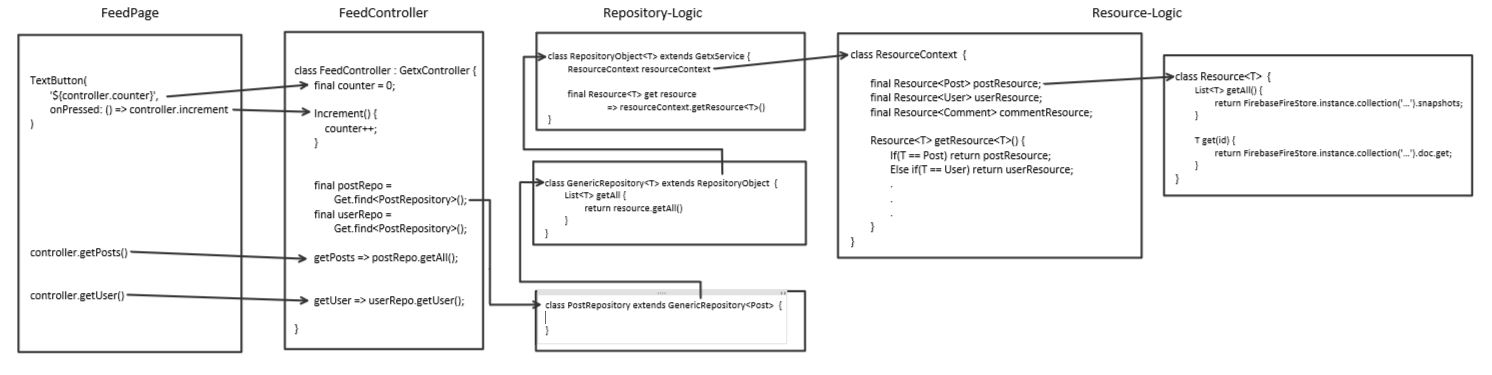
\includegraphics[width=1\textwidth]{pics/Repository-Resource-Diagram.jpg}
  \caption{Verwaltungslogik Diagramm}
  \label{fig:management-logic-diagram}
\end{figure}

Grafik wird noch verbessert.
\\
Die vorliegende Grafik \ref{fig:management-logic-diagram} stellt eine Struktur dar, die es ermöglicht Daten von einem Firestore-Server abzurufen und in einer Flutter-App zu verwalten. Die Struktur besteht aus mehreren Komponenten, die im Folgenden näher erläutert werden:
\\
Die Struktur beginnt auf der UI-Ebene mit der Seite, die Daten aus dem Firestore benötigt. Diese Seite verfügt über einen GetxController, der für die Verwaltung des Zustands und die Implementierung von Logik zuständig ist. Dieser Controller initialisiert Repositories, die den Zugriff auf die Daten vereinfachen.
\\
Jedes Repository erbt von einer GenericRepository-Klasse. Das GenericRepository ist ein generischer Typ, der es ermöglicht, Repositories für verschiedene Datenmodelle zu erstellen, ohne dass jeder Repository-Typ dieselben grundlegenden Operationen implementieren muss. Das bedeutet, dass ein Repository für jede Sammlung im Firestore erstellt werden kann, indem einfach der entsprechende Typ als generischer Parameter angegeben wird.
\\
Ein wichtiger Vorteil bei der Verwendung von generischen Repositories besteht darin, dass dadurch Code-Duplizierung vermieden wird. Durch die Implementierung von grundlegenden CRUD-Operationen in der GenericRepository-Klasse müssen diese nicht in jedem Repository wiederholt werden, was die Wartbarkeit des Codes erhöht und die Wahrscheinlichkeit von Fehlern verringert.
\\
Darüber hinaus ermöglicht die Verwendung von Generics auch die einfache Erweiterung und Anpassung der Implementierung. Wenn beispielsweise spezielle Anforderungen für bestimmte Datenmodelle bestehen, können diese problemlos in einem spezialisierten Repository hinzugefügt werden, ohne dass andere Teile des Codes beeinflusst werden.
\\
Die GenericRepository-Klasse erbt von der RepositoryObject-Klasse, welche den ResourceContext beinhaltet. Der ResourceContext stellt den Zugriff auf unterschiedliche Ressourcen bereit, wodurch die Interaktion mit den zugrunde liegenden Datenquellen ermöglicht wird.
\\
Jede Ressource ist für den Zugriff auf Daten einer entsprechenden Sammlung innerhalb des Firestore zuständig und implementiert grundlegende CRUD-Operationen. Durch die Kapselung dieser Operationen in dedizierten Ressourcen wird eine klare Trennung der Verantwortlichkeiten erreicht.
\\
Darüber hinaus erlaubt die Verwendung von ResourceContext eine einheitliche Schnittstelle für den Zugriff auf verschiedene Ressourcen, wodurch die Interoperabilität zwischen verschiedenen Komponenten der Verwaltungslogik gefördert wird. Diese Architektur erlaubt es, neue Ressourcen hinzuzufügen oder bestehende Ressourcen anzupassen, ohne die Gesamtstruktur der Anwendung zu beeinträchtigen.


\section{Flutter Packages}
\setauthor{Sandin Habibovic}

Im Folgenden finden Sie eine Auswahl an essentiellen und nützlichen Flutter-Pakete, die in der App zum Einsatz kam.
\\
\textbf{firebase\_core: \^2.0.0} - Dieses Paket bildet die grundlegende Firebase-Bibliothek, die für die Verwendung anderer Firebase-Pakete in der Appliaktion erforderlich ist. Initialisiert Firebase und stellt die Konfiguration bereit.
https://pub.dev/packages/firebase\_core
\\
\textbf{firebase\_auth: \^4.0.1} - Dieses Paket erlaubt die Integration der Firebase-Authentifizierung in der Applikation. Es unterstützt die Anmeldung mit verschiedenen Anbietern, wie beispielsweise E-Mail oder Google.
https://pub.dev/packages/firebase\_auth
\\
\textbf{cloud\_firestore: \^4.0.1} - Dieses Paket erlaubt die Integration von Firestore in der Applikation. Es unterstützt das Erstellen, Bearbeiten und Löschen von Daten in Echtzeit.
https://pub.dev/packages/cloud\_firestore
\\
\textbf{firebase\_storage: \^11.0.1} - Dieses Paket erlaubt die Integration von Cloud Storage in der Applikation. Es ermöglicht das Hoch- und Herunterladen von Dateien und Bildern.
https://pub.dev/packages/firebase\_storage
\\
\textbf{cloud\_functions: \^4.0.6} - Dieses Paket erlaubt die Verwendung von Cloud Functions in der Applikation. Wird für serverlose Logik und Backend-Integration verwendet.
https://pub.dev/packages/cloud\_functions
\\
\textbf{get: \^4.6.5} - Dieses Paket erlaubt die Integration von GetX in der Applikation. Es unterstützt das App-Management, die Navigation, die Zustandsverwaltung und Abhängigkeitsinjektionen.
https://pub.dev/packages/get
\\
\textbf{openai\_client: \^0.0.7} - Dieses Paket ermöglicht die Nutzung von OpenAI-Diensten in der Applikation, wodurch die Integration von künstlicher Intelligenz und maschinellem Lernen unterstützt wird.
https://pub.dev/packages/openai\_client
\\
\textbf{algolia: \^1.1.1} - Dieses Paket ermöglicht die Integration der Algolia-Suchplattform in der Applikation und bietet schnelle, relevante Suchergebnisse in Echtzeit.
https://pub.dev/packages/algolia
\\
\textbf{flutter\_map: \^3.1.0} - Dieses Paket ermöglicht die Integration von interaktiven Karten in der Applikation.
https://pub.dev/packages/flutter\_map
\\
\textbf{google\_mlkit\_translation: \^0.5.0} - Dieses Paket ermöglicht die Integration der Google ML Kit Translation-Funktion in der Applikation. Es unterstützt die Textübersetzungen in Echtzeit.
https://pub.dev/packages/google\_mlkit\_translation
\\
\textbf{google\_mlkit\_language\_id: \^0.5.0} - Dieses Paket ermöglicht die Integration der Googles ML Kit Language Identification in der Applikation. Es unterstützt die Identifizierung von Sprachen in Texten.
https://pub.dev/packages/google\_mlkit\_language\_id
\\
\textbf{google\_sign\_in: \^6.0.2} - Dieses Paket ermöglicht die Integration von Google Konten in der Applikation. Unterstützt die Google-Anmeldung.
https://pub.dev/packages/google\_sign\_in
\\
\textbf{feedback: \^2.5.0} - Dieses Paket ermöglicht das sammeln von Benutzerfeedback mit Screenshots und Anmerkungen, die an das Entwicklungsteam gesendet werden können.
https://pub.dev/packages/feedback
\\
\textbf{mobile\_scanner: \^3.0.0} - Dieses Paket ermöglicht die Integration von Scanner-Funktionalitäten für mobile Geräte in der Applikation und unterstützt das Scannen von Barcodes, QR-Codes und Dokumenten.
https://pub.dev/packages/mobile\_scanner
\\
\textbf{http: \^0.13.4} - Dieses Paket ermöglicht die Verwendung von HTTP-Anfragen in der Applikation. Es unterstützt GET, POST, PUT, DELETE und andere HTTP-Methoden.
https://pub.dev/packages/http
\\
\textbf{syncfusion\_flutter\_datepicker: \^20.2.45} - Dieses Paket ermöglicht die Verwendung von benutzerfreundlichen und anpassbaren Datumsauswahl-Funktionalitäten in der Applikation.
https://pub.dev/packages/syncfusion\_flutter\_datepicker
\\
\textbf{image: \^4.0.15} - Dieses Paket ermöglicht in der Applikation die Dekodierung, Bearbeitung und Kodierung von Bildern in verschiedenen Formaten wie PNG, JPEG, GIF und mehr.
https://pub.dev/packages/image
\\
\textbf{image\_picker: \^0.8.5+3} - Dieses Paket ermöglicht in der Appliaktion das Auswählen von Bildern aus der Galerie oder das Aufnehmen neuer Bilder mit der Kamera.
https://pub.dev/packages/image\_picker
\\
\textbf{image\_editor\_plus: \^0.2.0} - Dieses Paket ermöglicht in der Applikation eine einfach zu bedienende Bildbearbeitungs-Ansicht, das grundlegende Bearbeitungsfunktionen wie Zuschneiden, Drehen und Skalieren beherscht.
https://pub.dev/packages/image\_editor\_plus
\\
\textbf{cupertino\_icons: \^1.0.5} - Dieses Paket stellt eine Sammlung von über 1.000 hochwertigen iOS-Stil-Icons (Cupertino) für die Verwendung in der Applikation zur Verfügung.
https://pub.dev/packages/cupertino\_icons
\\
\textbf{get\_time\_ago: \^1.1.6:} - Dieses Paket ermöglicht in der Appliaktion das Umwandeln von Datumstypen in menschenlesbare Zeitangaben mit vordefinierbaren Layout.
https://pub.dev/packages/get\_time\_ago


\section{Visual Studio Code Extensions}
\setauthor{Martin Hausleitner}




\section{Email}
\setauthor{Martin Hausleitner}
Aufgrund des erhöhten E-Mail-Verkehrs des Teams nach dem Wettbewerb Linz haCKt musste eine Lösung gefunden werden, um diesen zentral zu verwalten. Aus diesem Grund wurde eine Gmail-Adresse erstellt, nämlich \href{mailto:project.locoo@gmail.com}{project.locoo@gmail.com}.

\subsection{Wechsel auf Nochba}
Als das Team von Locoo auf Nochba wechselte und eine .com- und .at-Domain erwarb, entstand die Idee, eine eigene E-Mail-Adresse zu erstellen. Beim Versuch, einen E-Mail-Server auf Azure selbst zu hosten, wurde schnell klar, dass dies nicht möglich war. Im Allgemeinen gestaltet sich das Hosten eines E-Mail-Servers schwierig, da viele Cloud-Anbieter dies nicht erlauben.

\subsection{Hosting-Anbieter}
Um den Aufwand zu minimieren, wurde der Hosting-Anbieter \cite{namecheap} ausgewählt, der ein sehr günstiges Angebot für ein Jahr E-Mail-Hosting hatte, bestehend aus 2 Monaten gratis und einem Jahr zum Preis von \$8.93.

\subsection{E-Mail-Adresse und Google-Account}
Die Entscheidung fiel auf die E-Mail-Adresse
\href{mailto:project@nochba.com}{project@nochba.com}, die mit dem DNS verbunden wurde.
Gleichzeitig wurde ein Google-Account erstellt, um alles
einheitlich mit der neuen E-Mail-Adresse zu gestalten.

\subsection{Zugang und Nutzung}
Das gesamte Team hatte Zugang zur E-Mail-Adresse und zum Webmail-Zugriff, obwohl die E-Mail-Adresse hauptsächlich von Martin Hausleitner und Arsham Edalatkhah genutzt wurde.

\subsection{Vorteile}
Rückblickend erwies sich die Entscheidung, eine eigene
E-Mail-Adresse zu erstellen, als äußerst vorteilhaft. Sie
vermittelte einen professionellen Eindruck und führte dazu,
dass das Projekt ernster genommen wurde. Zudem erleichterte
die eigene E-Mail-Adresse die Verwaltung von E-Mails an
einem zentralen Ort. Dies war besonders praktisch, da im


Laufe des Projekts verschiedene Anfragen eingingen und so
die Kommunikation effizienter gestaltet werden konnte.


\section{Visual Studio Code Extention}

Für die Programmierung einer App wurde das Werkzeug ChatGPT
eingesetzt, das auch nach der Veröffentlichung von
GPT-4relevanter wurde.  Eine einfache VSCode-Erweiterung
wurde entwickelt, um den Dart-Code zu minimieren. Da GPT-4
jedoch nur eine Eingabe von 8000 Tokens zulässt, ist es
schnell erreicht, wenn der Code nicht minimiert wird,
insbesondere wenn viele Leerzeichen aufgrund von
Einrückungen vorhanden sind. Jedes Leerzeichen stellt dabei
ein Token dar, was schnell zu einer Überschreitung der
maximalen Tokenanzahl führen kann. Die Erweiterung wurde
vollständig von GPT-4 programmiert und ist unter
\cite{copyminify} verfügbar.

Später wurde eine weitere Erweiterung programmiert, die die Anzahl der Tokens im aktuellen Code-File mithilfe von Codex oder GPT-3 Tokenizer anzeigt. Wenn ein bestimmter Bereich im Code-File ausgewählt ist, wird nur die Anzahl der Tokens in diesem Bereich angezeigt. Die Erweiterung wurde im VSCode Marketplace veröffentlicht und ist unter \cite{tokenizer} erhältlich.


\section{Zukünftige mögliche implementierungen}
Das Ziel des Teams besteht darin, die App jedem Österreicher und jeder Österreicherin zugänglich zu machen, weshalb die Entwicklung noch lange nicht abgeschlossen ist. Aus diesem Grund wurden im Folgenden einige Ideen aufgelistet, die während des Brainstormings entstanden sind.


\begin{itemize}
  \item App soll komplett auf Open-Source-Plattformen basieren
  \item Neuentwicklung der App
  \item Supabase statt Firebase verwenden
\end{itemize}

\subsection{Benutzererfahrung (UX) und Benutzeroberfläche (UI)}
\begin{itemize}
  \item UI/UX-Überarbeitung
  \item Eigenes UI-Package für die App
  \item Vereinfachung der Beitragserstellung
  \item Automatische Kategorisierung von Beiträgen durch KI
  \item Anpassbare Benachrichtigungseinstellungen
  \item Erweiterte persönliche Daten im Profil
\end{itemize}

\subsection{Registrierung und Profil}
\begin{itemize}
  \item Vereinfachung des Registrierungsprozesses
        \begin{itemize}
          \item Adressen-Autocomplete
        \end{itemize}
  \item Identitätsverifizierung mit Ausweis
  \item Weitere Verifizierungsmöglichkeiten
\end{itemize}

\subsection{Kommunikation und Interaktion}
\begin{itemize}
  \item Neuentwicklung des Chats
        \begin{itemize}
          \item Gruppenchats
          \item Chat-Reaktionen
          \item Sprachnachrichten
          \item Beiträge in Chats versenden
          \item Google ML Kit Entity Extraction
          \item Chat-Übersetzung
          \item Erweiterte Anhangsoptionen: Standort
        \end{itemize}
  \item Punktesystem wie Karma auf Reddit, um fleißige Nachbarn zu belohnen
  \item Zusätzliche Karma-Belohnungen für Reaktionen
  \item Weitere Kategorien, z.B. Umfragen
  \item Übersicht aller Nachbarn in der Umgebung
  \item In-App-Moderation und Berichterstattung unangemessener Inhalte
  \item Integration von Veranstaltungskalendern und lokalen Events
  \item Nachbarschaftsprojekte und gemeinsame Aktivitäten vorschlagen
  \item Lokale Geschäfts- und Serviceempfehlungen
\end{itemize}

\subsection{Internationalisierung und Übersetzungen}
\begin{itemize}
  \item App in mehreren Sprachen übersetzen
  \item Automatische Übersetzung für alle Teile der App
\end{itemize}

\subsection{Hilfe und Support}
\begin{itemize}
  \item Erweiterte Hilfe und Tutorials
  \item Erweiterte Einstellungsmöglichkeiten
\end{itemize}

\subsection{Technische Verbesserungen}
\begin{itemize}
  \item Umfangreiches Caching in der App
  \item Chat-Verschlüsselung
  \item Deep Links für jede Seite
  \item Einladecodes mit Links
\end{itemize}

\subsection{Sicherheit und Datenschutz}
\begin{itemize}
  \item Erweiterte Sicherheitsmechanismen
  \item Erweiterte Benachrichtigungsoptionen
\end{itemize}

